\documentclass[handout]{beamer}
\usepackage{geometry}
%\geometry{a4paper}
\usepackage[utf8]{inputenc}
\usepackage{amsmath,amssymb}
\usepackage{hyperref} % verlinkungen
\usepackage{textcomp}
\usepackage{flafter}
\usepackage{booktabs}
\usepackage{array}
\usepackage{paralist}
\usepackage{dsfont} \usepackage{color}
\usepackage{bbold}
\usepackage{float}
\usepackage[font=scriptsize,labelfont=bf]{caption}
%\usepackage[font=footnotesize,labelfont=bf]{caption}
\usepackage[font=scriptsize]{subcaption}
\usepackage{fancyhdr}
\setlength{\headheight}{15.2pt}
\pagestyle{empty}
\usepackage{listings} 
\usepackage{pict2e}
\usepackage{xfrac}
\usepackage[german]{babel}
\usepackage{mathtools}
\usepackage{graphicx}
\usepackage{pdfpages}
\usetheme{Madrid}
\usepackage{wrapfig}
\mode<handout>
{
  \usepackage{pgf}
  \usepackage{pgfpages}

\pgfpagesdeclarelayout{4 on 1 boxed}
{
  \edef\pgfpageoptionheight{\the\paperheight} 
  \edef\pgfpageoptionwidth{\the\paperwidth}
  \edef\pgfpageoptionborder{0pt}
}
{
  \pgfpagesphysicalpageoptions
  {%
    logical pages=4,%
    physical height=\pgfpageoptionheight,%
    physical width=\pgfpageoptionwidth%
  }
  \pgfpageslogicalpageoptions{1}
  {%
    border code=\pgfsetlinewidth{2pt}\pgfstroke,%
    border shrink=\pgfpageoptionborder,%
    resized width=.5\pgfphysicalwidth,%
    resized height=.5\pgfphysicalheight,%
    center=\pgfpoint{.25\pgfphysicalwidth}{.75\pgfphysicalheight}%
  }%
  \pgfpageslogicalpageoptions{2}
  {%
    border code=\pgfsetlinewidth{2pt}\pgfstroke,%
    border shrink=\pgfpageoptionborder,%
    resized width=.5\pgfphysicalwidth,%
    resized height=.5\pgfphysicalheight,%
    center=\pgfpoint{.75\pgfphysicalwidth}{.75\pgfphysicalheight}%
  }%
  \pgfpageslogicalpageoptions{3}
  {%
    border code=\pgfsetlinewidth{2pt}\pgfstroke,%
    border shrink=\pgfpageoptionborder,%
    resized width=.5\pgfphysicalwidth,%
    resized height=.5\pgfphysicalheight,%
    center=\pgfpoint{.25\pgfphysicalwidth}{.25\pgfphysicalheight}%
  }%
  \pgfpageslogicalpageoptions{4}
  {%
    border code=\pgfsetlinewidth{2pt}\pgfstroke,%
    border shrink=\pgfpageoptionborder,%
    resized width=.5\pgfphysicalwidth,%
    resized height=.5\pgfphysicalheight,%
    center=\pgfpoint{.75\pgfphysicalwidth}{.25\pgfphysicalheight}%
  }%
}


  \pgfpagesuselayout{4 on 1 boxed}[a4paper, border shrink=5mm, landscape]
  \nofiles
}


%%%%%%%%         EIGENEBEFEHLE  %%%%%%%%%
\newcommand{\ddt}{\frac{\partial}{\partial{t}}}
\newcommand{\dnach}[1]{\frac{\partial}{\partial{#1}}}
\newcommand{\ddnach}[2]{\frac{\partial{#1}}{\partial{#2}}}
\newcommand{\dddnach}[3]{\frac{\partial^2{#1}}{\partial{#2} \partial{#3}}}
\newcommand{\dznach}[2]{\frac{\partial^2{#1}}{\partial{#2}^2}}
\newcommand{\vnabla}{\mathbf{\nabla}}
\newcommand{\emathbf}[1]{\mathbf{\hat{#1}}}
\newcommand{\bra}[1]{\langle{#1}|}
\newcommand{\ket}[1]{|{#1}\rangle}
\newcommand{\bracket}[2]{\langle{#1}|{#2}\rangle}
\newcommand{\up}{\uparrow}
\newcommand{\down}{\downarrow}
\newcommand{\updown}{\uparrow\downarrow}
\newcommand{\downup}{\downarrow\uparrow}
\newcommand{\upup}{\uparrow\uparrow}
\newcommand{\downdown}{\downarrow\downarrow}
\newcommand{\sandwich}[2]{\bra{#1} #2 \ket{#1}}
\newcommand{\fsqrt}[2]{\sqrt{\frac{#1}{#2}}}
\newcommand{\GammaK}{{\Gamma_k}}

\definecolor{mygreen}{rgb}{0,0.6,0}
\definecolor{mygray}{rgb}{0.5,0.5,0.5}
\definecolor{mymauve}{rgb}{0.58,0,0.82}

\lstset{%
  backgroundcolor=\color{white},   % choose the background color; you must add \usepackage{color} or \usepackage{xcolor}
  basicstyle=\footnotesize,        % the size of the fonts that are used for the code
  breakatwhitespace=false,         % sets if automatic breaks should only happen at whitespace
  breaklines=true,                 % sets automatic line breaking
  captionpos=b,                    % sets the caption-position to bottom
  commentstyle=\color{mygreen},    % comment style
  %deletekeywords={...},            % if you want to delete keywords from the given language
  %escapeinside={\%*}{*)},          % if you want to add LaTeX within your code
  extendedchars=true,              % lets you use non-ASCII characters; for 8-bits encodings only, does not work with UTF-8
  frame=single,                    % adds a frame around the code
  keepspaces=true,                 % keeps spaces in text, useful for keeping indentation of code (possibly needs columns=flexible)
  keywordstyle=\color{blue},       % keyword style
  language=C,                 % the language of the code
  %morekeywords={*,...},            % if you want to add more keywords to the set
  numbers=left,                    % where to put the line-numbers; possible values are (none, left, right)
  numbersep=5pt,                   % how far the line-numbers are from the code
  numberstyle=\tiny\color{mygray}, % the style that is used for the line-numbers
  rulecolor=\color{black},         % if not set, the frame-color may be changed on line-breaks within not-black text (e.g. comments (green here))
  showspaces=false,                % show spaces everywhere adding particular underscores; it overrides 'showstringspaces'
  showstringspaces=false,          % underline spaces within strings only
  showtabs=false,                  % show tabs within strings adding particular underscores
  stepnumber=2,                    % the step between two line-numbers. If it's 1, each line will be numbered
  stringstyle=\color{mymauve},     % string literal style
  tabsize=2,                       % sets default tabsize to 2 spaces
  %title=\lstname                   % show the filename of files included with \lstinputlisting; also try caption instead of title
}

\lhead[\ ]{\leftmark }
\chead[\ ]{\ }
\rhead[\ ]{\rightmark }

\lfoot[\ ]{\ }
\cfoot[\ ]{\thepage }
\rfoot[\ ]{\ }

%%%%%%%%%%%%%%%%%%%%%%%%%%%%%%%%%%%%%%%%%%%%

\begin{document}
\AtBeginSection[]{
  \begin{frame}
  \vfill
  \centering
  \begin{beamercolorbox}[sep=8pt,center,shadow=true,rounded=true]{title}
    \usebeamerfont{title}\insertsectionhead\par%
  \end{beamercolorbox}
  \vfill
  \end{frame}
}
\title{Simulation of Nano Particles in a Laser Trap}
%\subtitle{Präsentation der Masterarbeit}
\author{Mathias Höld, BSc}
\date{23.03.2017}
\begin{frame}
\titlepage
\end{frame}

\setbeamertemplate{section in toc}{\inserttocsection}
\begin{frame}
\tableofcontents
\end{frame}

\section{Einleitung}
\begin{frame}
\frametitle{Einleitung}
Verbindung von zwei Teilbereichen der Physik:
\begin{itemize}
\item Computational Physics
\item Optische Fallen
\end{itemize}
\end{frame}

\begin{frame}
\frametitle{Computational Physics}
\begin{itemize}
\item Meilenstein: Entwicklung des Metropolis Monte Calro Algoithmus (1953)
\item Seit dem enorme Verbesserung der Rechenleistung von Computern 
\item Neue Methoden entwickelt (Transition Path Sampling, Finite-Elemente,\ldots)
\item In dieser Arbeit verwendet: Molekulardynamik-Simulation
\end{itemize}
\end{frame}

\begin{frame}
\frametitle{Optische Fallen}
\begin{itemize}
\item Lokalisierung von Objekten durch Gradientenkraft eines Laserstrahls
\item Objekte von subatomarer bis Mikrometer-Skala
\item Erste Idee zu Beginn des 20. Jahrhunderts (Lebedev, Nichols, Hull)
\item Realisierung 1970 durch Ashkin
\end{itemize}
\end{frame}

\section{Motivation}
\subsection{Experiment -- Gieseler et al.}
\begin{frame}
\frametitle{Experiment -- Gieseler et al.}
\begin{center}
\begin{figure}
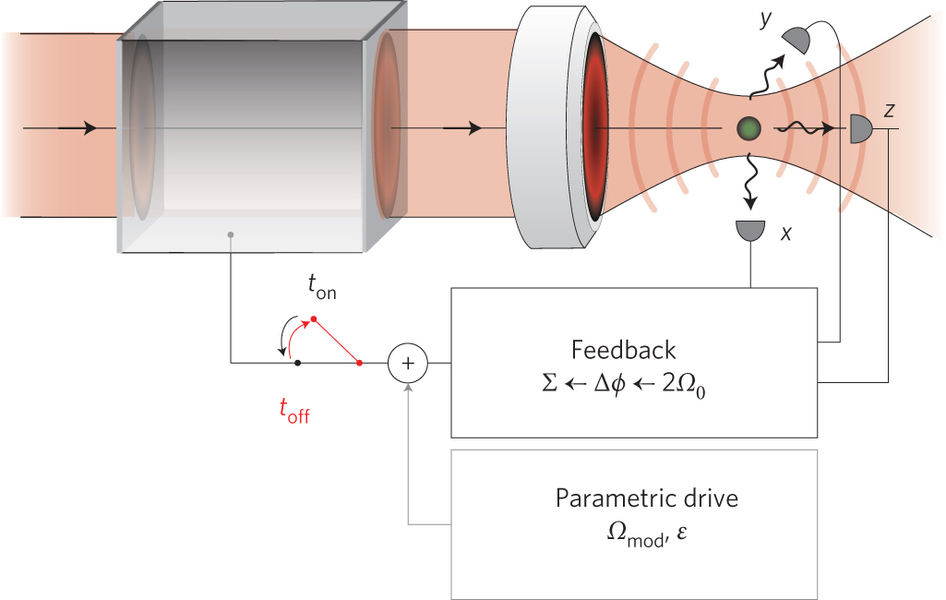
\includegraphics[scale=0.3]{../images/experimental_setup.jpg}
\caption{Experimenteller Aufbau \cite{Gieseler2014}}
\end{figure}
\end{center}
\end{frame}

\begin{frame}
\frametitle{Bewegungsgleichung}
1-D Langevin-Gleichung:
\begin{equation}
    \label{eq:langevin}
    \ddot{x} + \Gamma_0 \dot{x} + \Omega^2_0x = \frac 1 m \left(F_\text{fluct} + F_\text{ext}\right)
\end{equation}
\begin{tabular}{l l}
$x$ & Ort des Teilchens\\
$\dot{x}$ & Geschwindigkeit des Teilchens\\
$\ddot{x}$ & Beschleunigung des Teilchens\\
$m$ & Masse des Teilchens\\
$\Gamma_0$ & Reibungskoeffizient\\
$\Omega_0$ & Winkelfrequenz (Fluktuation)\\
$F_\text{fluct}$ & stochastische Kraft\\
$F_\text{ext}$ & externe Kraft
\end{tabular}
\end{frame}

\begin{frame}
\frametitle{Stochastische Kraft}
Stochastische Kraft:
\begin{equation}
    \label{eq:ffluct}
    F_\text{fluct} = \sqrt{2m\Gamma_0k_BT_0} \ \xi\left(t\right)
\end{equation}
\begin{tabular}{l l}
$T$ & Temperatur Wärmereservoir\\
$k_B$ & Boltzmann-Konstante\\
$\xi(t)$ & Weißes Rauschen\\
\end{tabular}\\
\end{frame}

\begin{frame}
\frametitle{Fluktuationstheorem}
Fluktuationstheorem für diese Situation:
\begin{equation}
    \label{eq:fluctuationtheorem}
    \frac{p(-\Delta S)}{\Delta S} = e^{-\Delta S}
\end{equation}
%\end{frame}
%\begin{frame}
%\frametitle{Fluktuationstheorem}
$\Delta S$: relative Entropieänderung
\begin{equation}
    \Delta S = \beta_0 Q + \Delta \phi
\end{equation}
\begin{tabular}{l l}
$Q$ & absorbierte Wärme\\
$\beta$ & reziproke Temperatur\\
$\Delta \phi$ & Differenz der trajektoriebasierten Entropie
\end{tabular}\\
Untersucht für 2 externe Kräfte: Feedback-Mechanismus ohne und mit Parametrischem Drive
\end{frame}

\subsection{Temperaturmodell}
\begin{frame}
\frametitle{Experiment -- Millen et al.}
\begin{center}
\begin{figure}
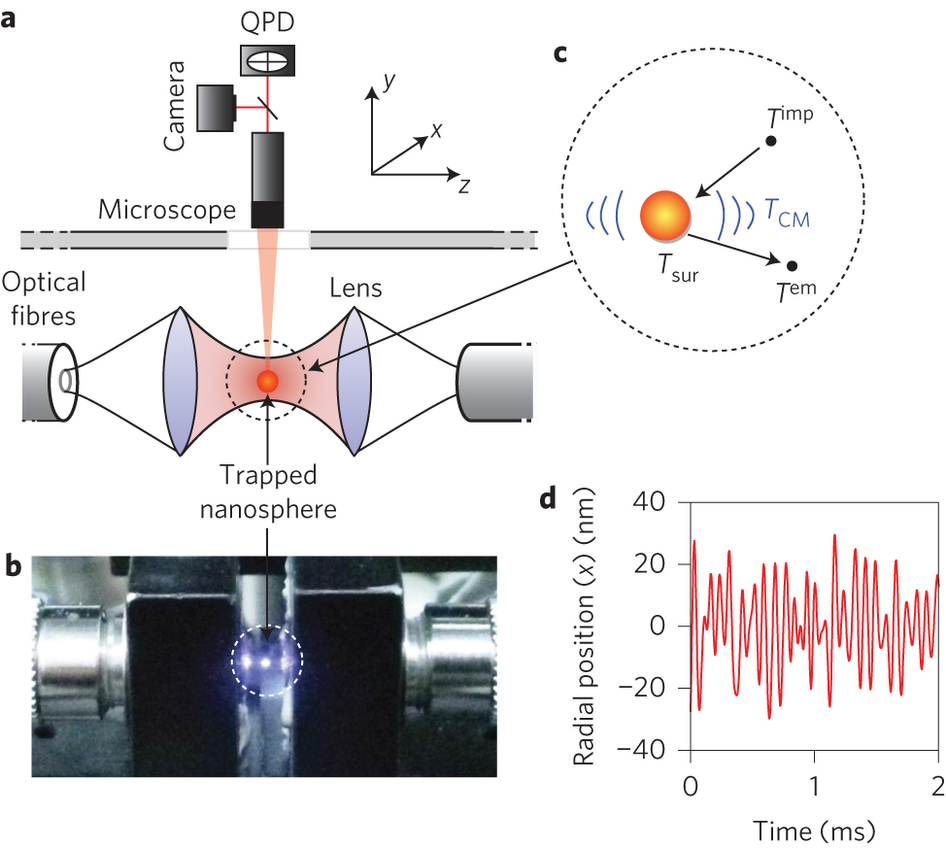
\includegraphics[scale=0.2]{../images/nnano_millen.jpg}
\caption{Experimenteller Aufbau \cite{MillenJ.2014}}
\end{figure}
\end{center}
\end{frame}

\begin{frame}
\frametitle{Temperaturen}
4 unterschiedliche Temperaturen:
\begin{itemize}
\item Schwerpunktstemperatur $T_\text{COM}$
\item Oberflächentemperatur$T_\text{sur}$
\item Temperatur eingehendes Gas $T_\text{imp}$
\item Temperatur ausgehendes Gas $T_\text{em}$
\end{itemize}
\end{frame}

\begin{frame}
\frametitle{Wärmereservoire des umgebenden Gases}
\begin{center}
\begin{figure}
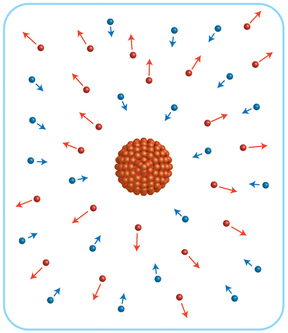
\includegraphics[scale=0.4]{../images/nano_nonequilibrium_cropped.jpg}
\caption{Wärmereservoire des umgebenden Gases \cite{Kroy2014}}
\end{figure}
\end{center}
\end{frame}


\begin{frame}
\frametitle{Modifizierte Bewegungsgleichung}
Modifizierte 1-D Langevin-Gleichung:
\begin{equation}
    M\ddot{x}(t) + M\left(\Gamma^\text{imp}+\Gamma^\text{em}\right)\dot{x}(t) + M\omega^2x(t) =F^\text{imp}+F^\text{em}
\end{equation}
\begin{tabular}{l l}
$x$ & Ort des Teilchens\\
$\dot{x}$ & Geschwindigkeit des Teilchens\\
$\ddot{x}$ & Beschleunigung des Teilchens\\
$M$ & Masse des Teilchens\\
$\Gamma^\text{imp/em}$ & Reibungskoeffizient eingehendes/ausgehendes Gas\\
$\omega$ & Winkelfrequenz (Fluktuation)\\
$F^\text{imp/em}$ & Noise-Term eingehendes/ausgehendes Gas
\end{tabular}
\end{frame}

\begin{frame}
\frametitle{Fragestellung}
Mit Einführung der unterschiedlichen Temperaturen stellen sich folgende Fragen:
\begin{itemize}
\item Welchen Einfluss hat die Laserintensität auf die Schwerpunktsbewegung des Teilchens in der Falle?
\item Welchen Einfluss hat die Temperatur des Umgebenden Gases?
\end{itemize}
\end{frame}



\section{Simulation}

\subsection{Velocity Verlet}
\begin{frame}
\frametitle{Velocity Verlet}
Integration der Newton'schen Bewegungsgleichungen durch Velocity Verlet Algorithmus:
\begin{equation}
    \label{eq:velocityverlet}
    \begin{aligned}
        \mathbf{r}_i(t+\Delta t) = \mathbf{r}_i(t) + {\mathbf{v}}_i(t) \Delta t + \frac1{2m} {\mathbf{F}}_i(t) \Delta t^2\\
        \mathbf{v}_i(t+\Delta t) = \mathbf{v}_i(t) + \frac1{2m} \Big[\mathbf{F}_i(t) + \mathbf{F}_i(t+\Delta t)\Big] \Delta t
    \end{aligned}
\end{equation}
\begin{tabular}{l l}
$\mathbf{r}_i$ & Position Teilchen $i$\\
$\mathbf{v}_i$ & Geschwindigkeit Teilchen $i$\\
$\mathbf{F}_i$ & Kraft auf Teilchen $i$\\
$\Delta t$ & Zeitschritt\\
\end{tabular}\\
\end{frame}

\subsection{Nanoteilchen}

\begin{frame}
\frametitle{Nanoteilchen}
Nanoteilchen dargestellt durch System aus $N$ Teilchen, die über Lennard-Jones Potential wechselwirken:
\begin{equation}
    \label{eq:lj}
    U(r) = 4\varepsilon\left[\left(\frac\sigma r\right)^{12} - \left(\frac\sigma r\right)^6\right]
\end{equation}
\begin{tabular}{l l}
$\varepsilon$ & Potentialtiefe\\
$\sigma$ & Abstand, wo Potential Null ist\\
$r$ & Intermolekularer Abstand\\
\end{tabular}\\
\end{frame}

\begin{frame}
\frametitle{Lennard-Jones Potential}
\begin{center}
\begin{figure}
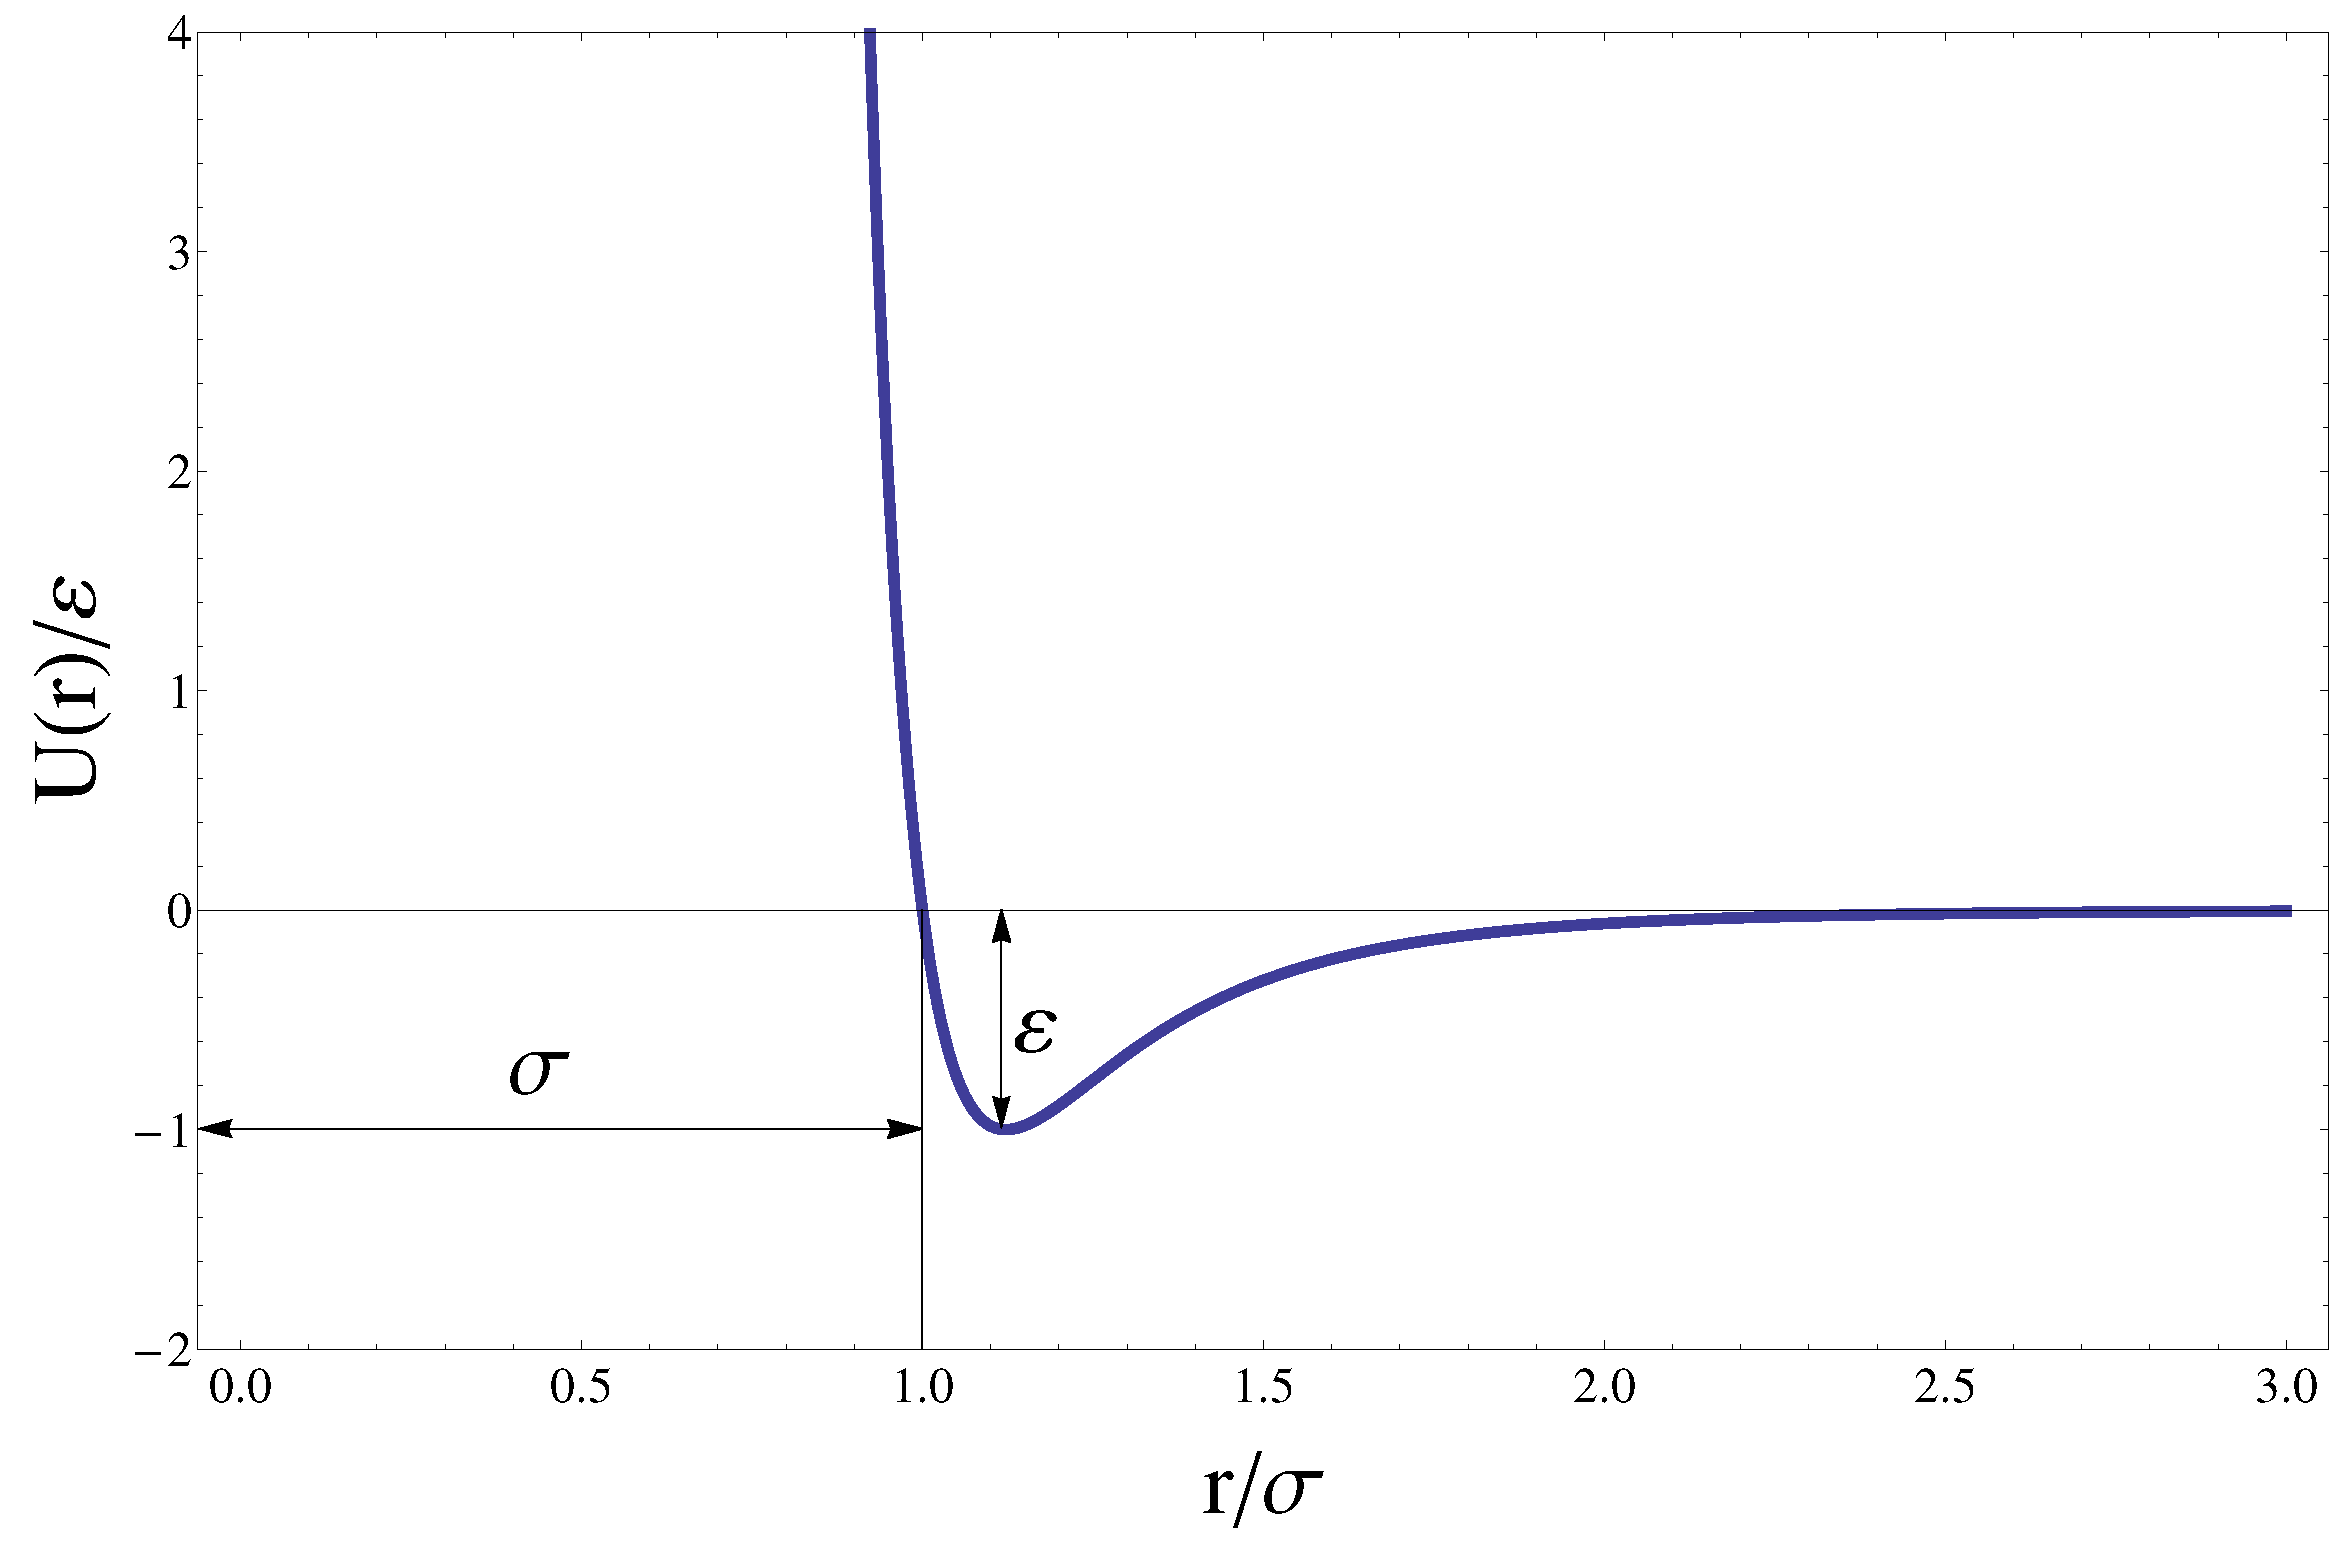
\includegraphics[scale=0.3]{../images/LJ-2.pdf}
\end{figure}
\end{center}
\end{frame}

\begin{frame}
\frametitle{Reduzierte Einheiten}
Um Rechnung zu vereinfachen, werden reduzierte Einheiten verwendet:
\begin{itemize}
\item Länge: $\sigma$ $\rightarrow$ $r^* = r/\sigma$
\item Energie: $\varepsilon$ $\rightarrow$ $U^* = U/\varepsilon$
\item Masse: $m$
\end{itemize}
Lennard-Jones Potential und zugehörige Kraft in reduzierten Einheiten:
\begin{eqnarray}
    U(r) &=& 4\left[{r}^{-12} - {r}^{-6}\right] \\
    F_{x} &=& -\frac{\partial}{\partial x} U(r) = 48 \left[r^{-14} - 0.5 \ r^{-8}\right] x
\end{eqnarray}
\end{frame}



\subsection{Laserstrahl -- Wärmequelle}
\begin{frame}
\frametitle{Laserstrahl -- Wärmequelle}
Simulation der Aufnahme von Wärme des Lasers: eHEX (enhanced Heat Exchange Algorithm)\\
Idee: sukzessive Reskalierung der Geschwindigkeiten 
\begin{equation}
    \mathbf{v}_i \rightarrow \mathbf{\bar{v}}_i = \xi_k \mathbf{v}_i
\end{equation}
kombiniert mit Velocity Verlet

\end{frame}

\subsection{Laserstrahl -- Lokalisierung}
\begin{frame} 
\frametitle{Laserstrahl -- Lokalisierung}
Lokalisierung des Teilchens durch Laserstrahl: Harmonisches Potential
\begin{eqnarray}
    \mathbf{F} &=& -k \Big[\mathbf{r}_\text{COM}-\mathbf{x}_0\Big]\\
    U &=& \frac12 k \Big[\mathbf{r}_\text{COM}-\mathbf{x}_0\Big]^2
\end{eqnarray}
\begin{tabular}{l l}
$\mathbf{r_\text{COM}}$ & Schwerpunktsposition\\
$\mathbf{x_0}$ & Minimum des Potentials\\
$k$ & Federkonstante\\
\end{tabular}\\
\end{frame}

\subsection{Umgebendes Gas -- Thermostat}
\begin{frame}
\frametitle{Umgebendes Gas -- Thermostat}
Ideales Gas als Druckmedium mit Interaktionspotential
\begin{equation}
    \label{eq:softsphere}
    U(r) = \varepsilon \left(\frac{\sigma}{r}\right)^{12}
\end{equation}
\begin{tabular}{l l}
$\varepsilon$ & Interaktionsstärke\\
$\sigma$ & Interaktionslänge\\
\end{tabular}\\
\end{frame}

\begin{frame}
\frametitle{Algorithmus}
Wichtige Elemente des Algorithmus:
\begin{itemize}
\item Nanoteilchen umgeben von Volumen
\item Eingefügte Teilchenanzahl pro Fläche: 
\begin{equation}
    \langle N_\text{fac}\rangle = \Delta t L^2 P \sqrt{\frac{1}{2\pi m k_B T}}
\end{equation}
\item Geschwindigkeitskomponente Normal zur Fläche
\begin{equation}
    p(v_i) = \frac{m}{k_B T}v_i \ e^{-\frac{mv_i^2}{2k_BT}}
\end{equation}
\item Andere Komponenten: Maxwell-Boltzmann
\end{itemize}
\end{frame}

\section{Ergebnisse}

\begin{frame}
\frametitle{Ergebnisse -- Überblick}
\begin{figure}[h]
    \begin{center}
        \begin{subfigure}[t]{0.3\textwidth}
            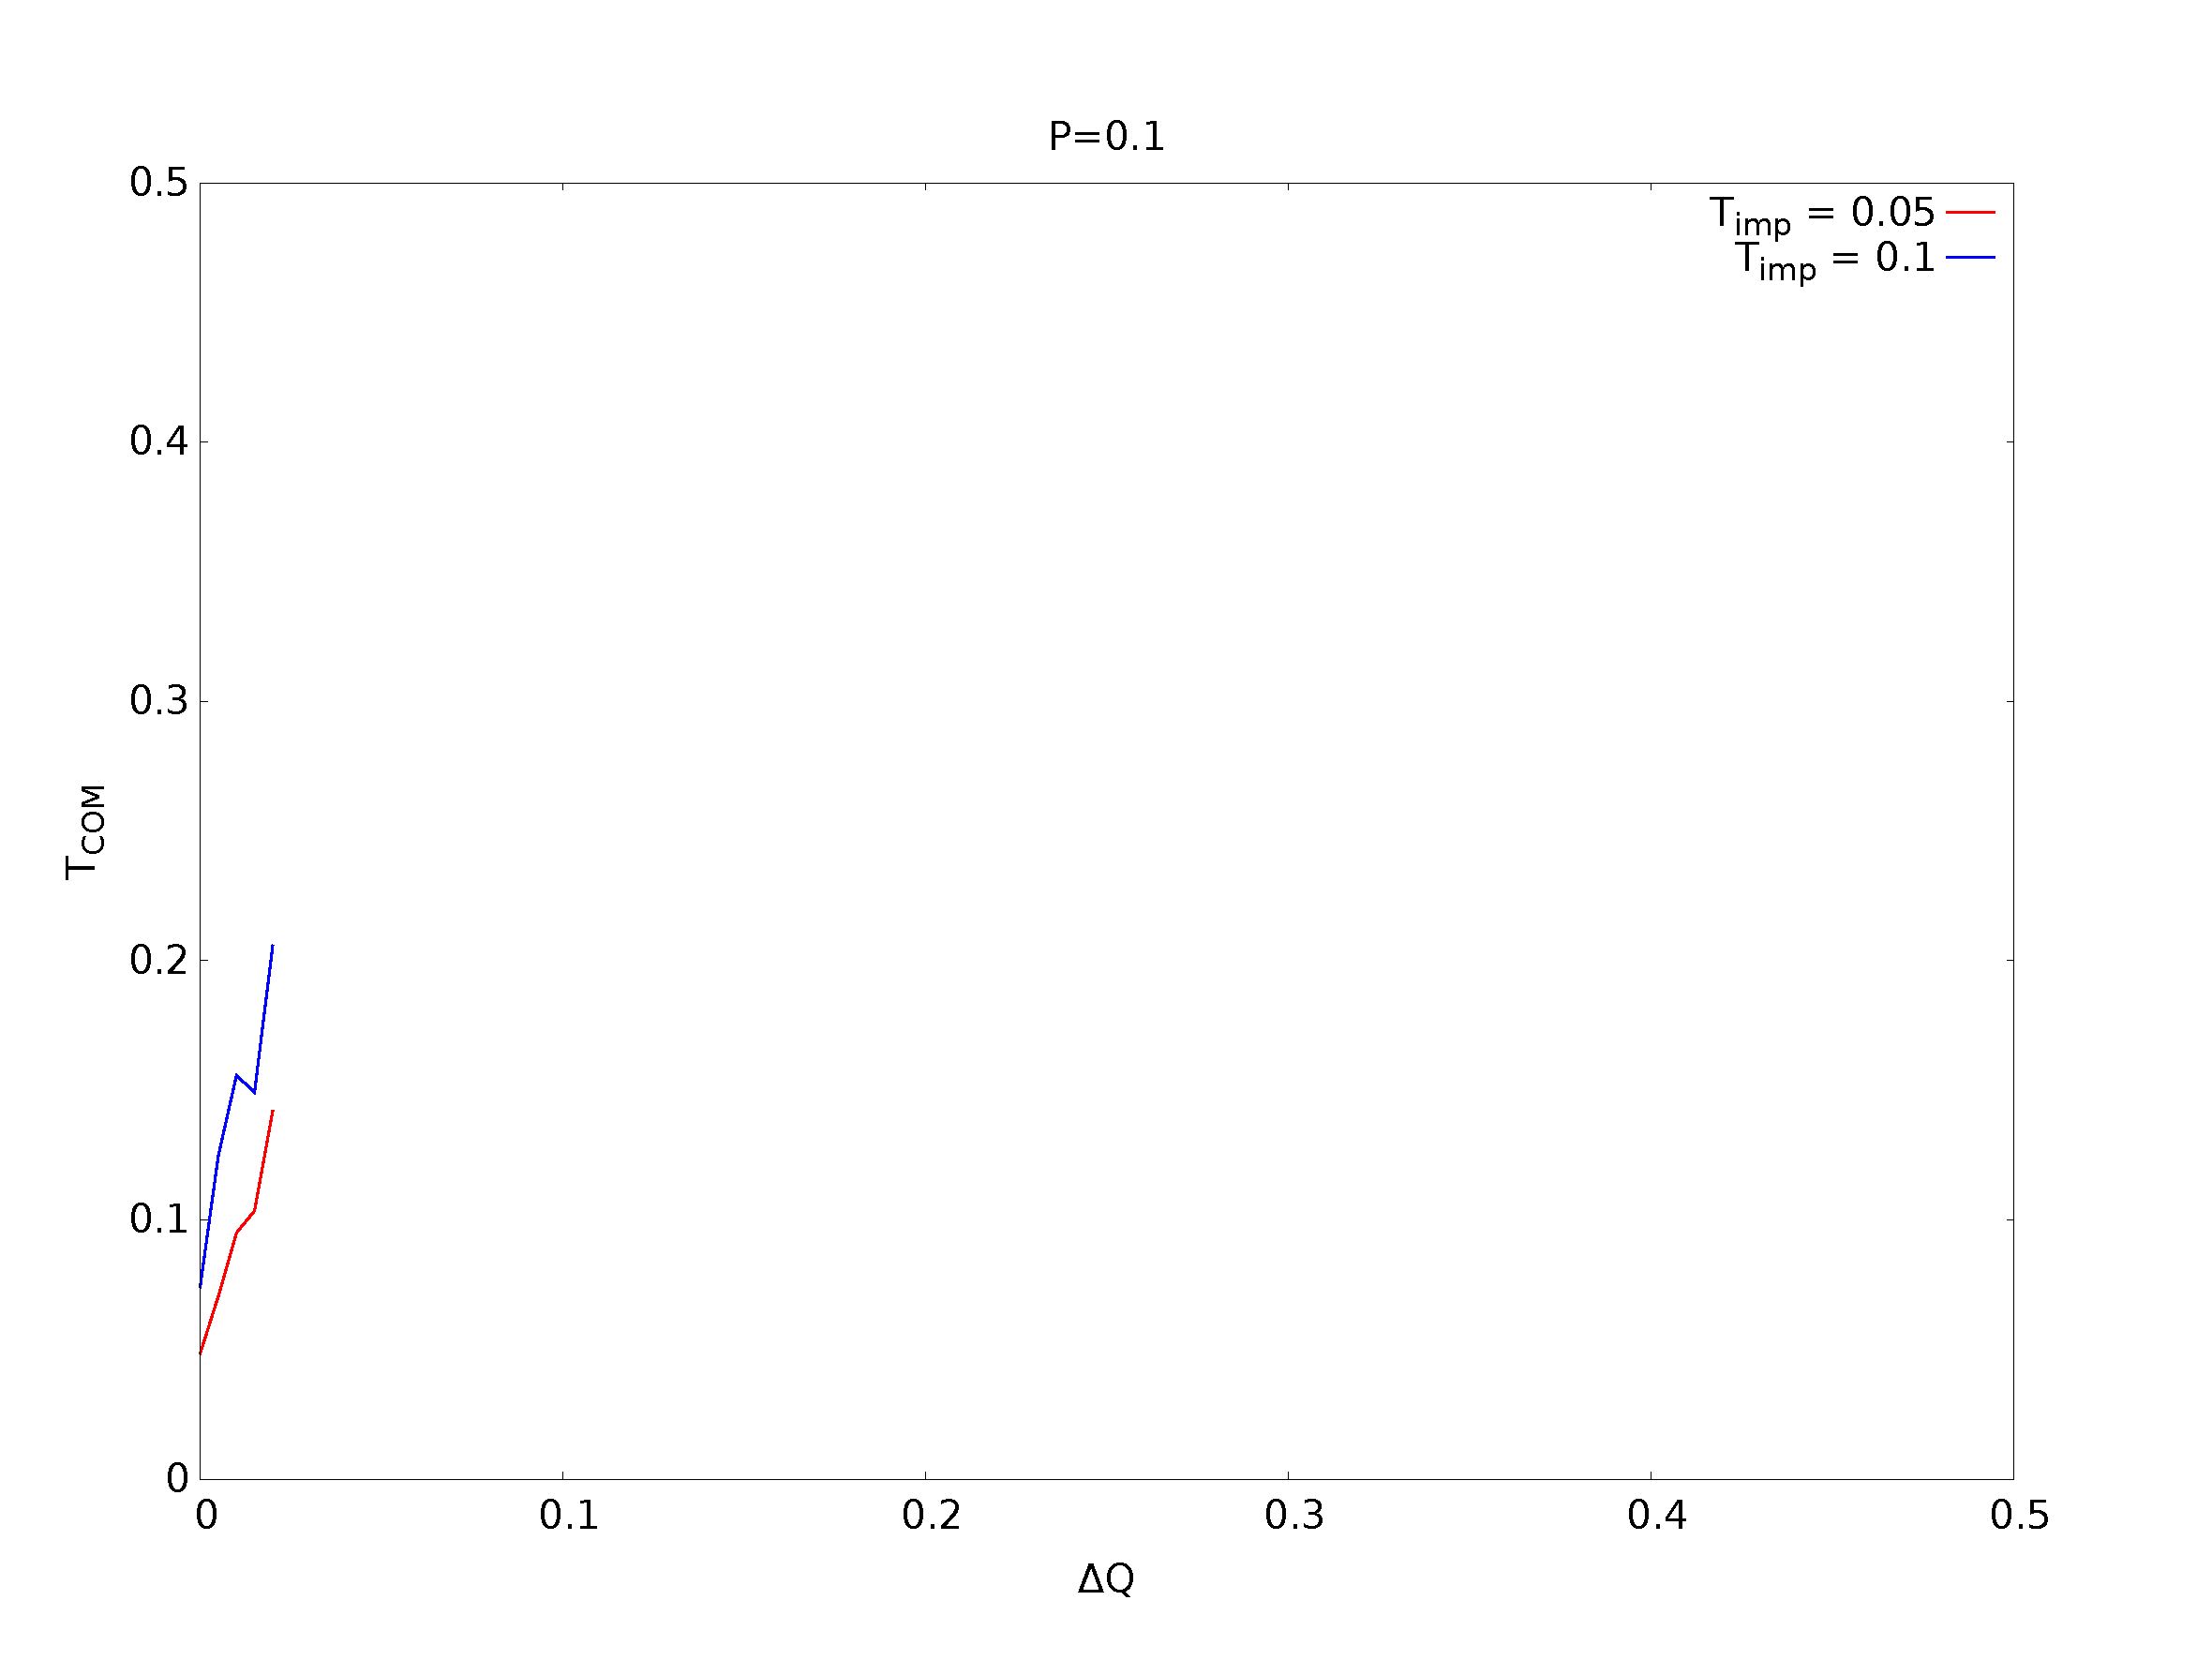
\includegraphics[scale=0.09]{../images/p01_com.pdf}
        \end{subfigure} 
        \
        \begin{subfigure}[t]{0.3\textwidth}
            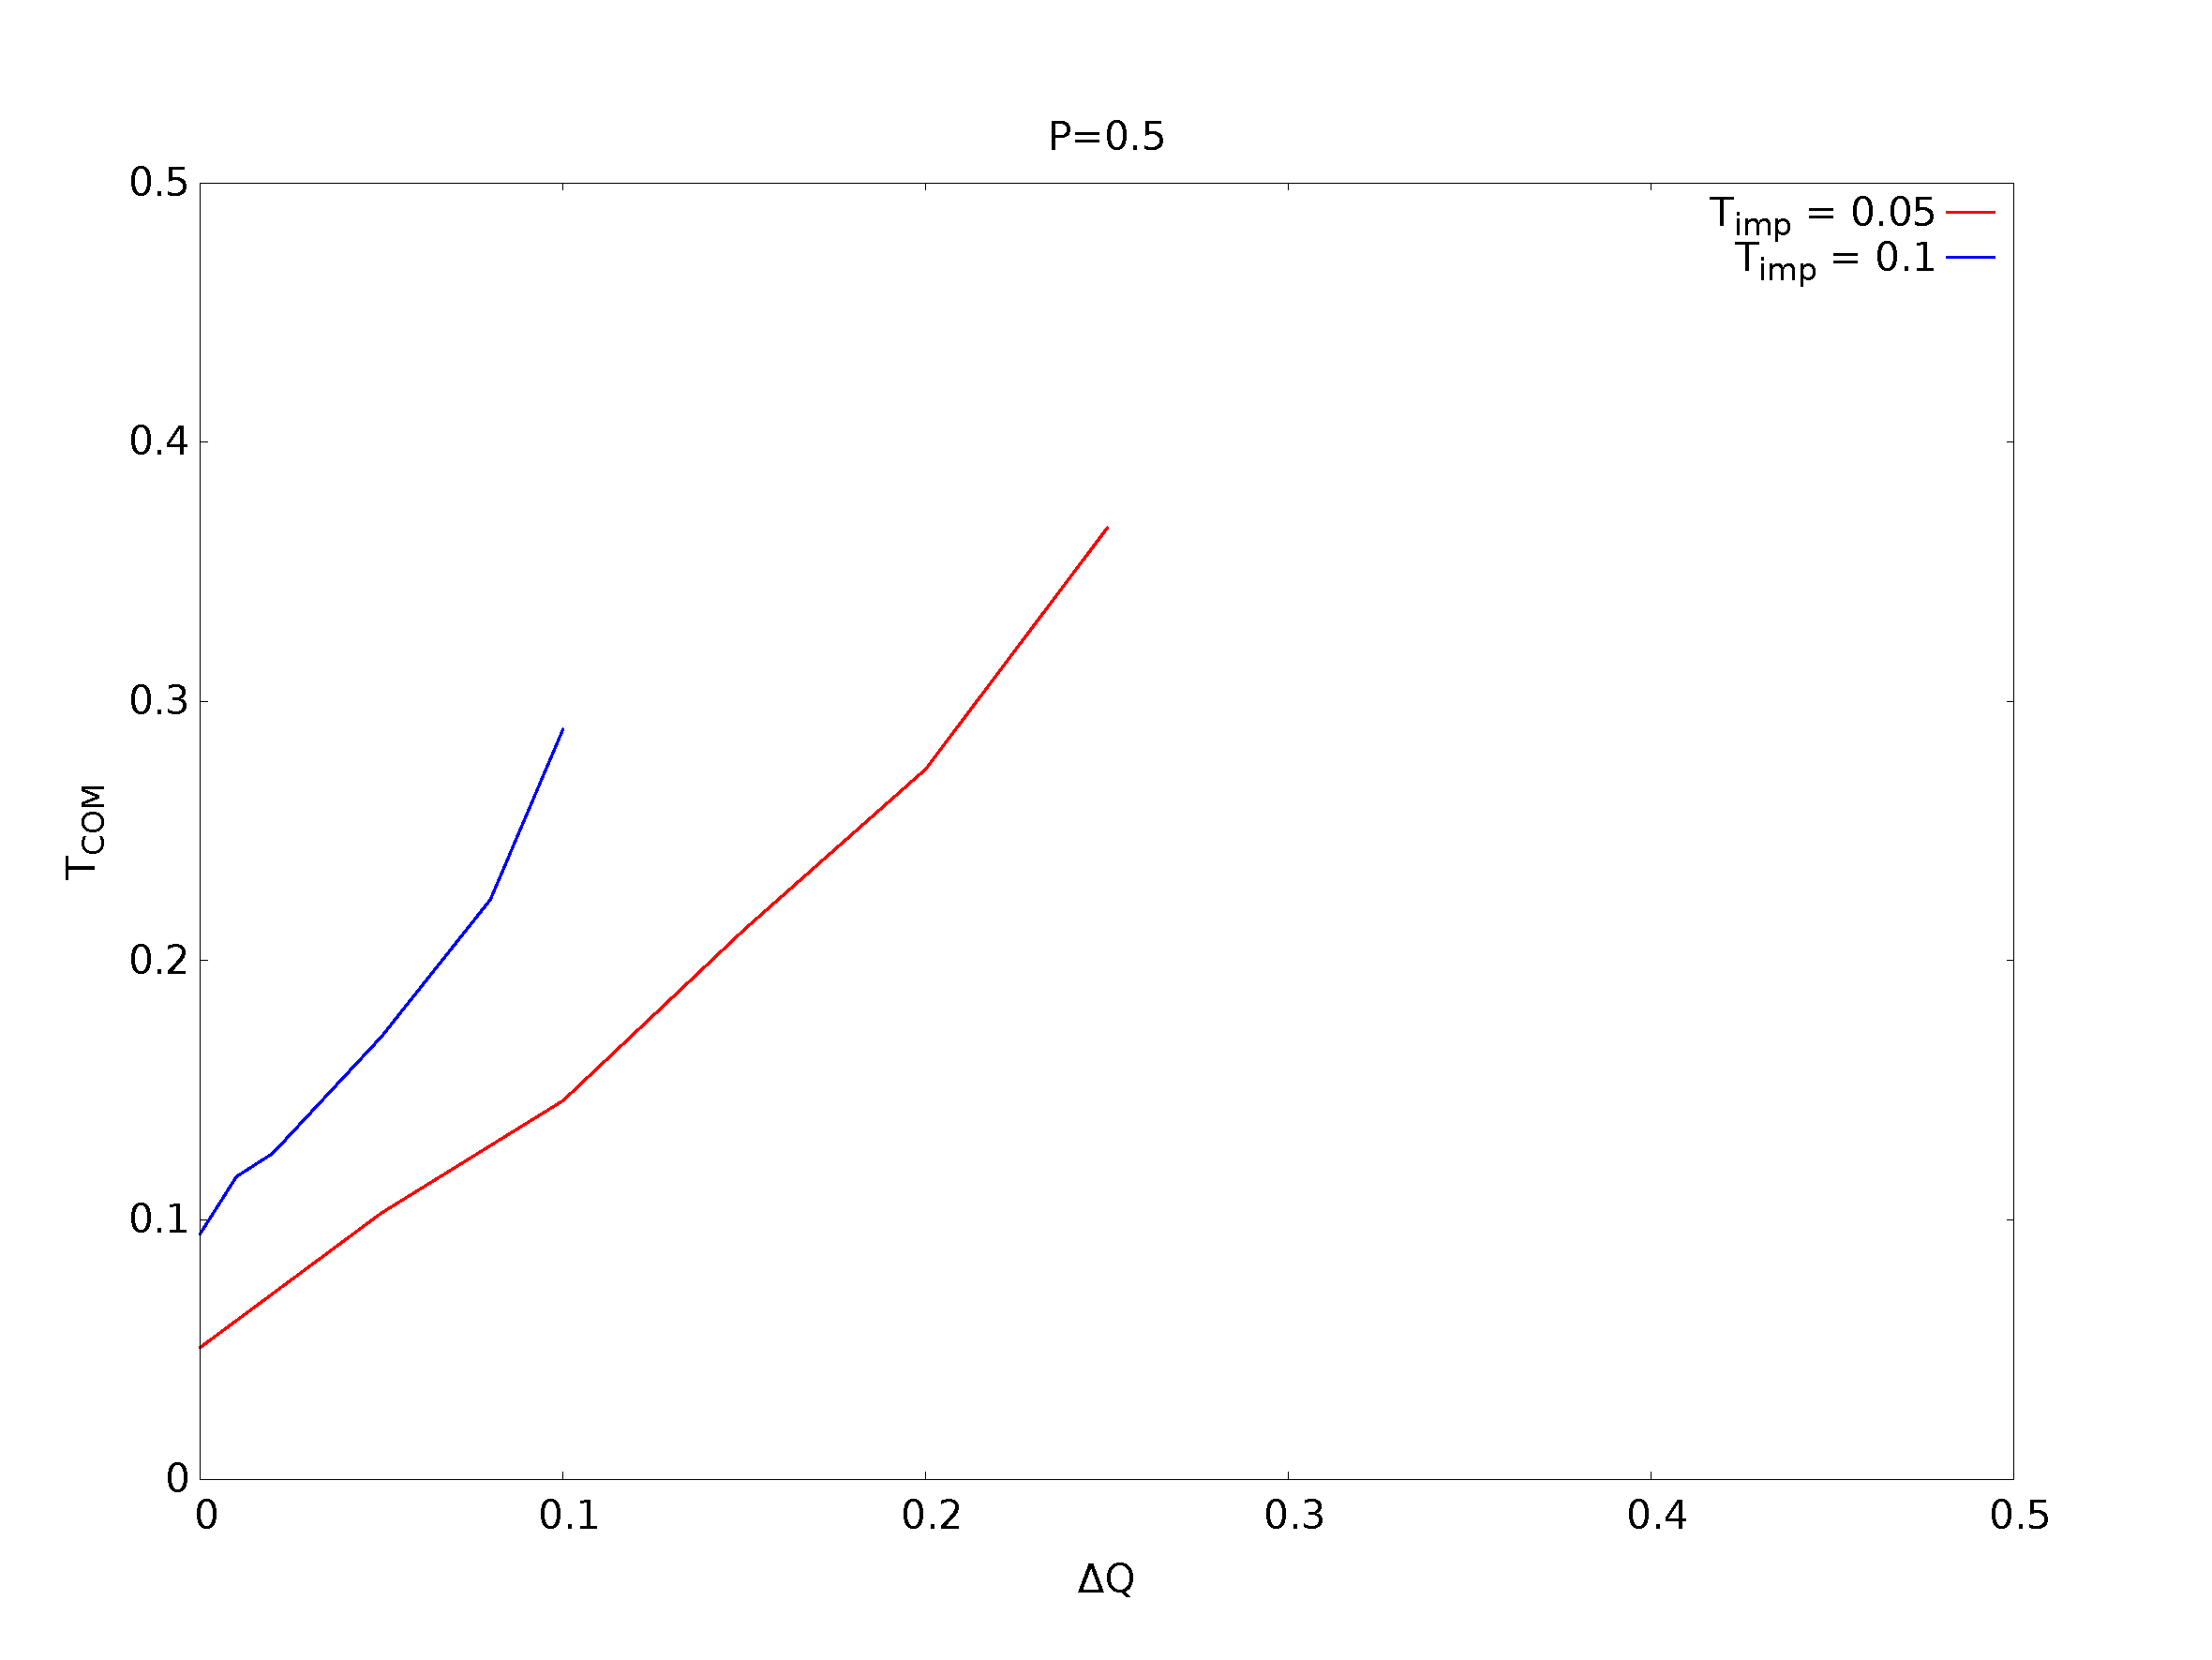
\includegraphics[scale=0.09]{../images/p05_com.pdf}
        \end{subfigure} 
        \
        \begin{subfigure}[t]{0.3\textwidth}
            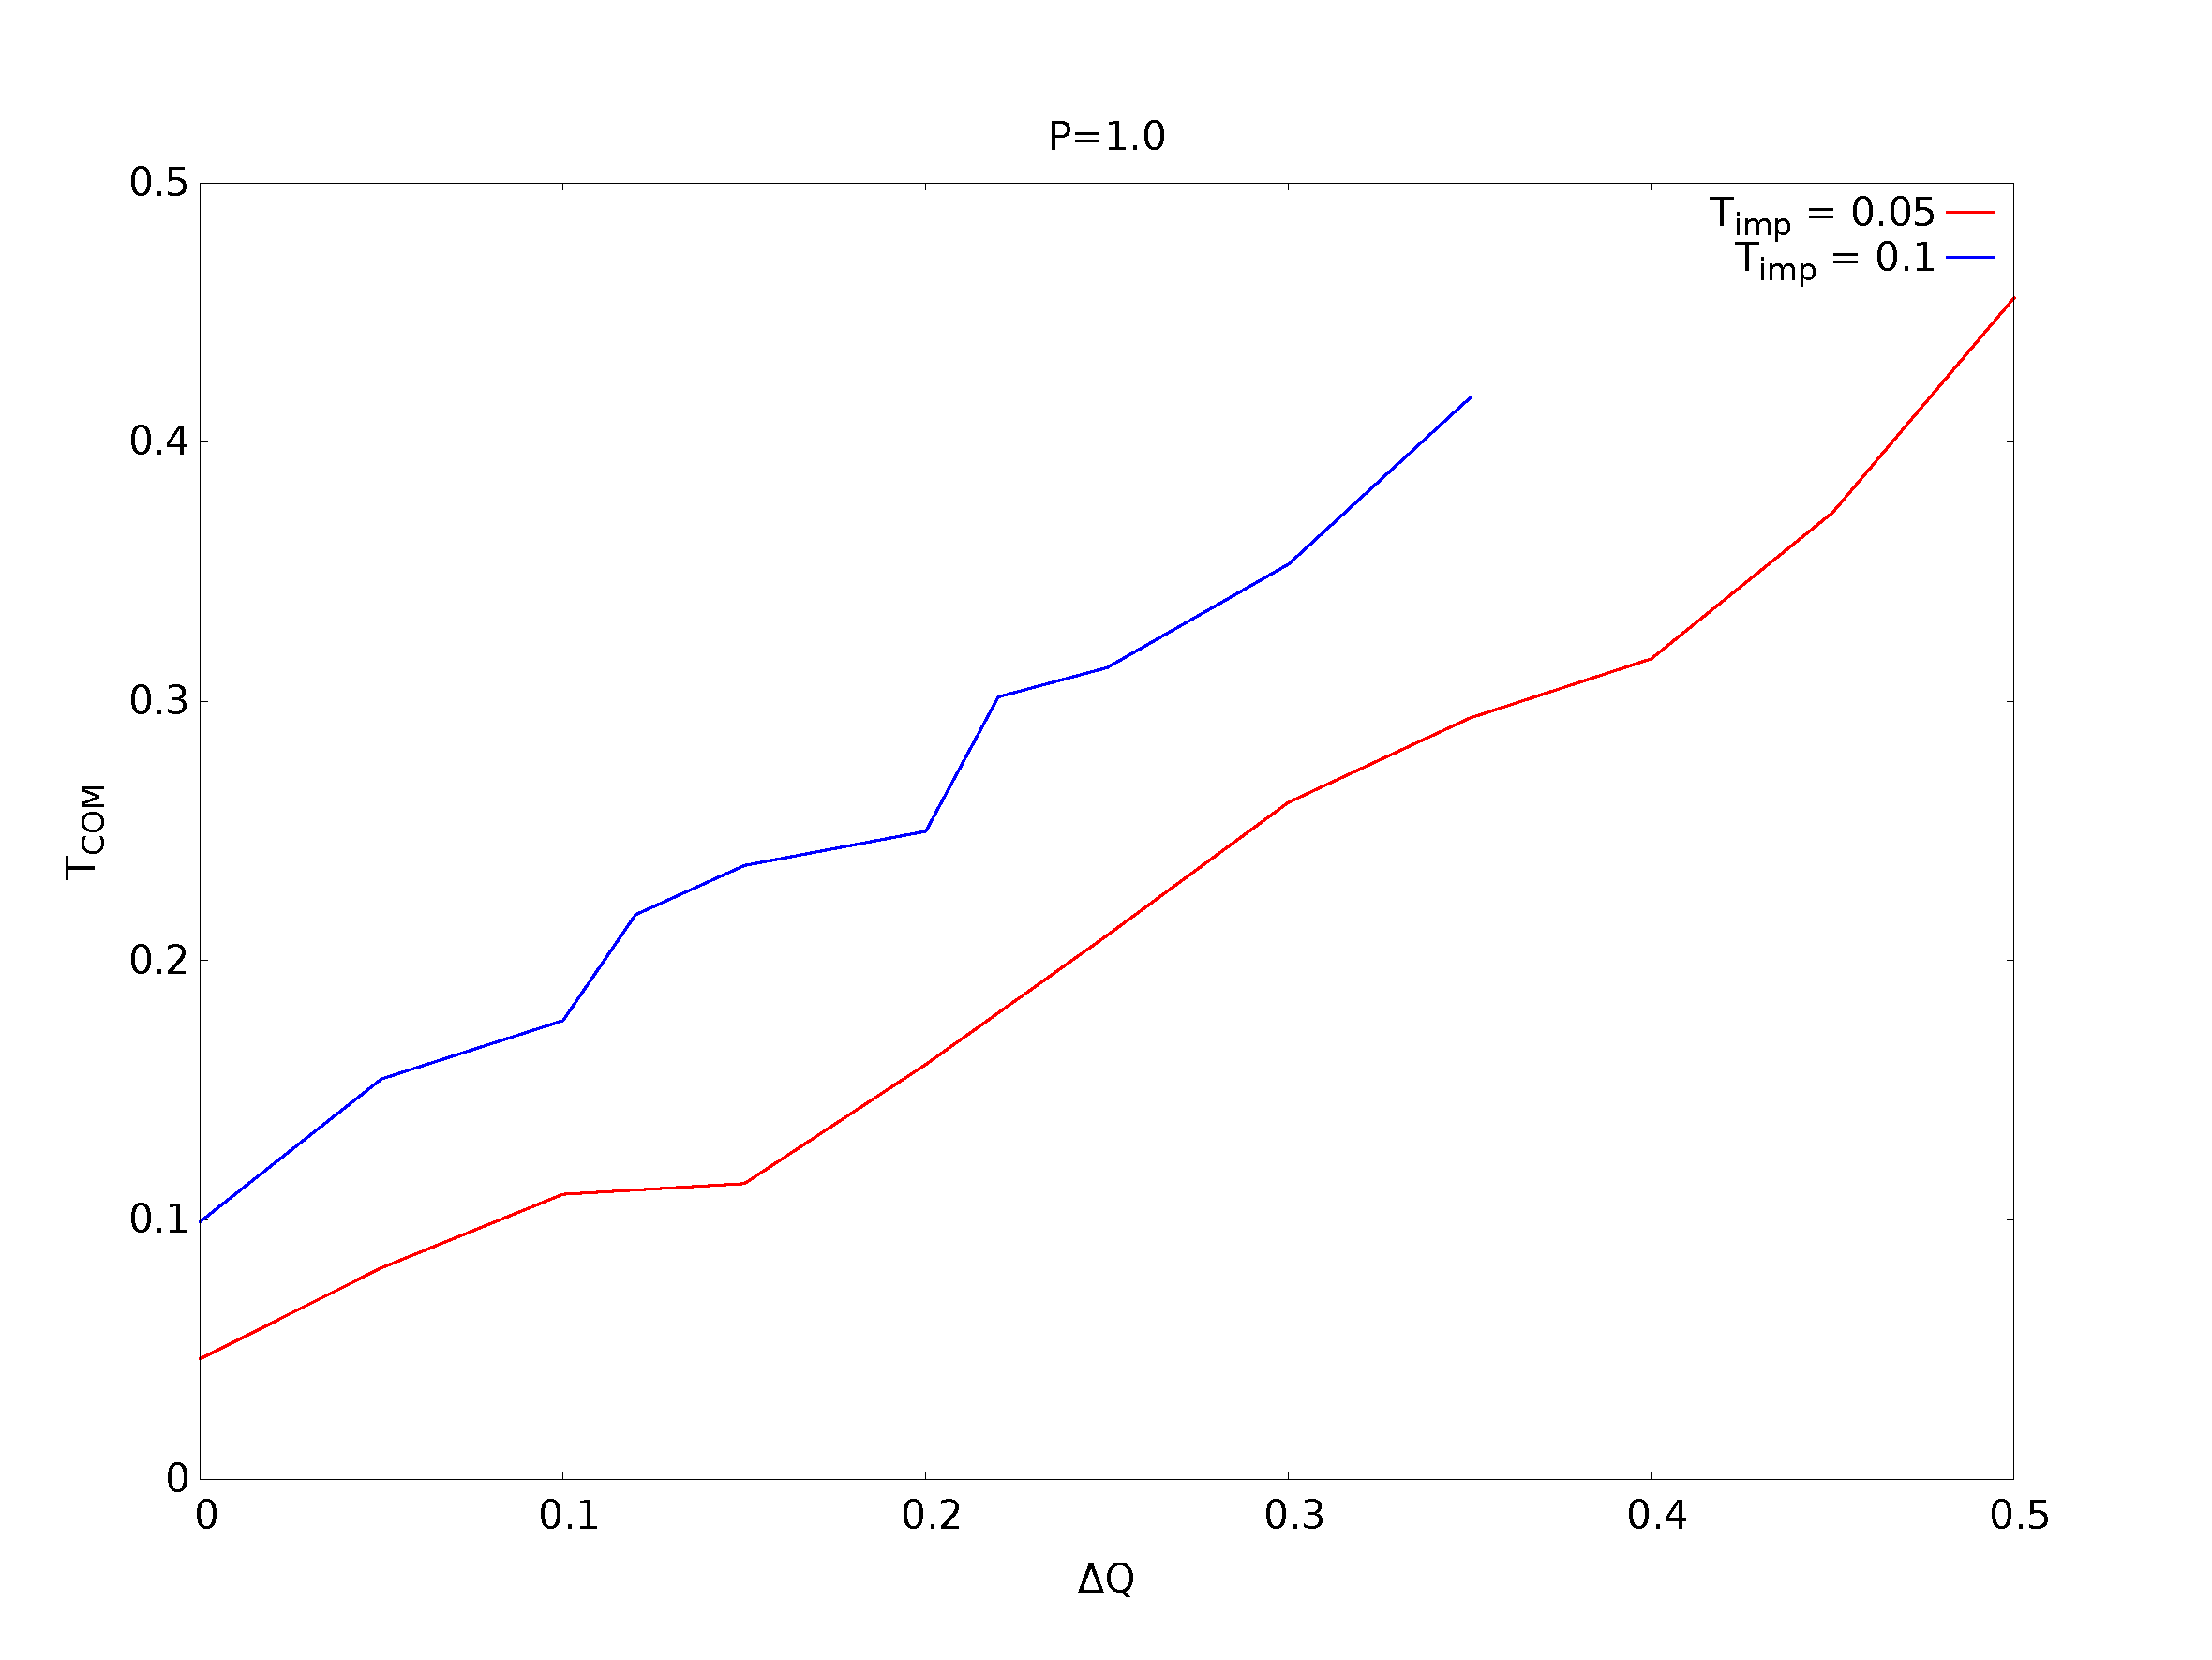
\includegraphics[scale=0.09]{../images/p1_com.pdf}
        \end{subfigure} 
        \\
        \begin{subfigure}[t]{0.3\textwidth}
            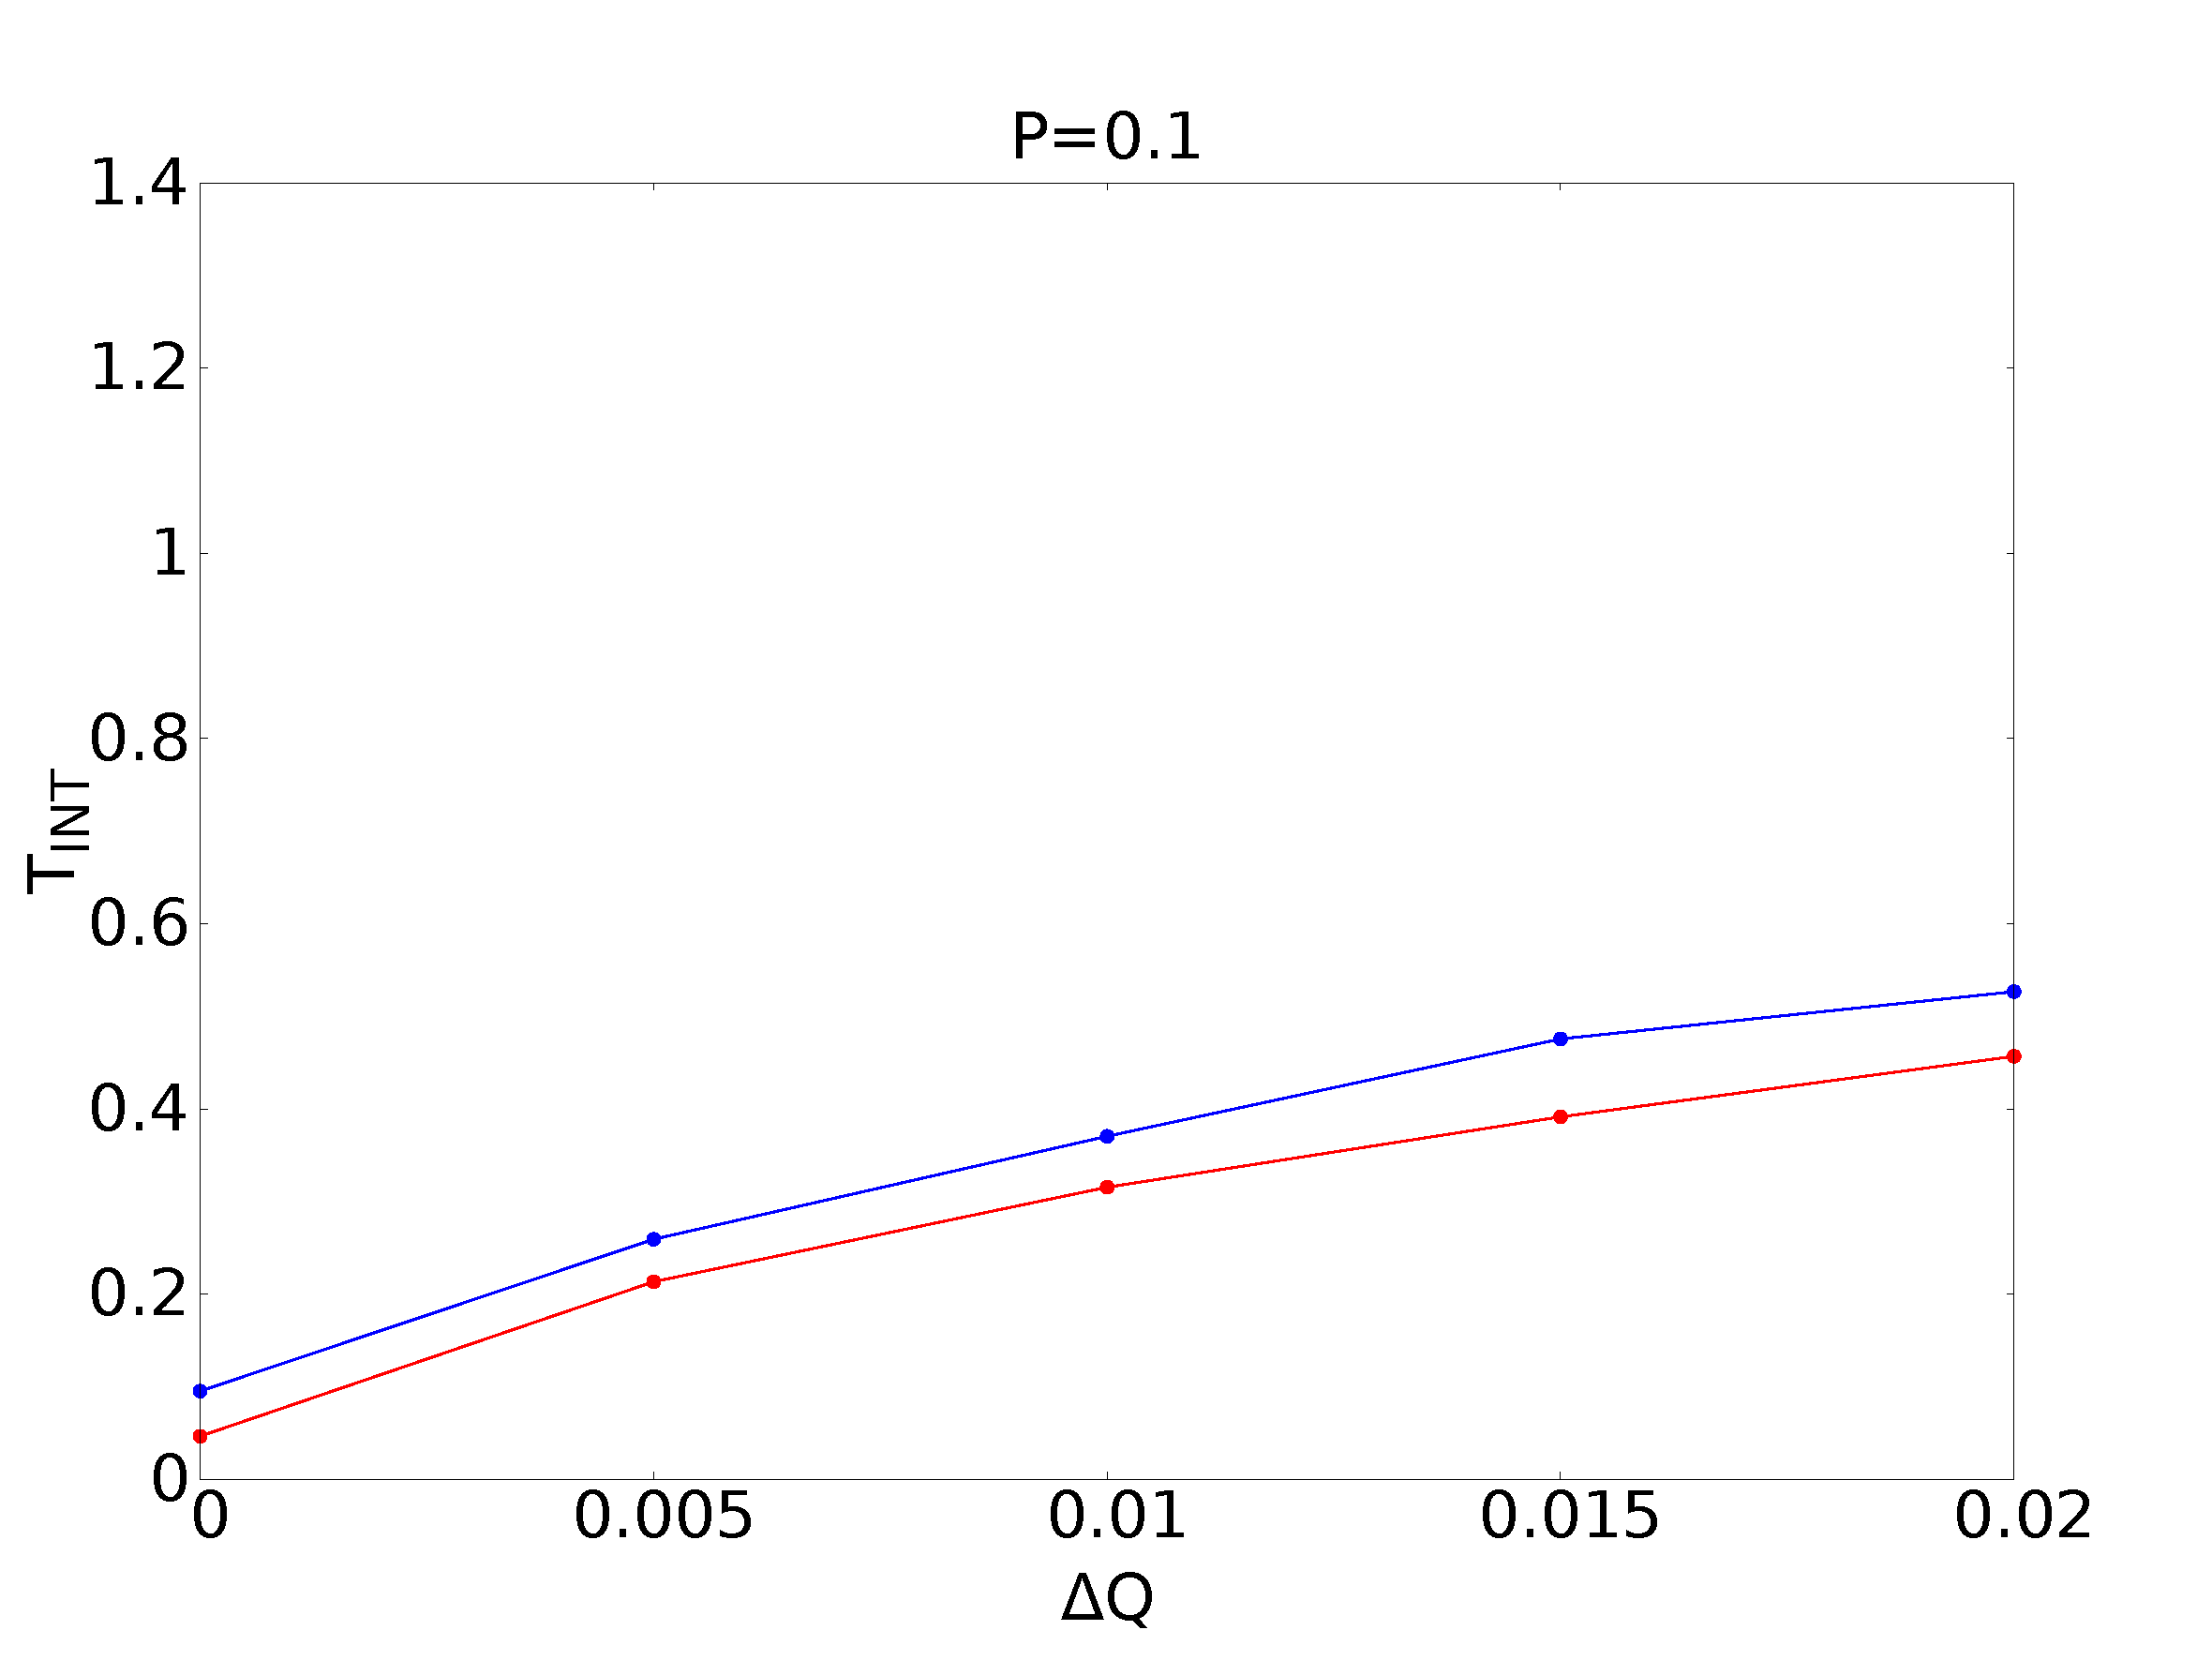
\includegraphics[scale=0.09]{../images/p01_int.pdf}
        \end{subfigure} 
        \
        \begin{subfigure}[t]{0.3\textwidth}
            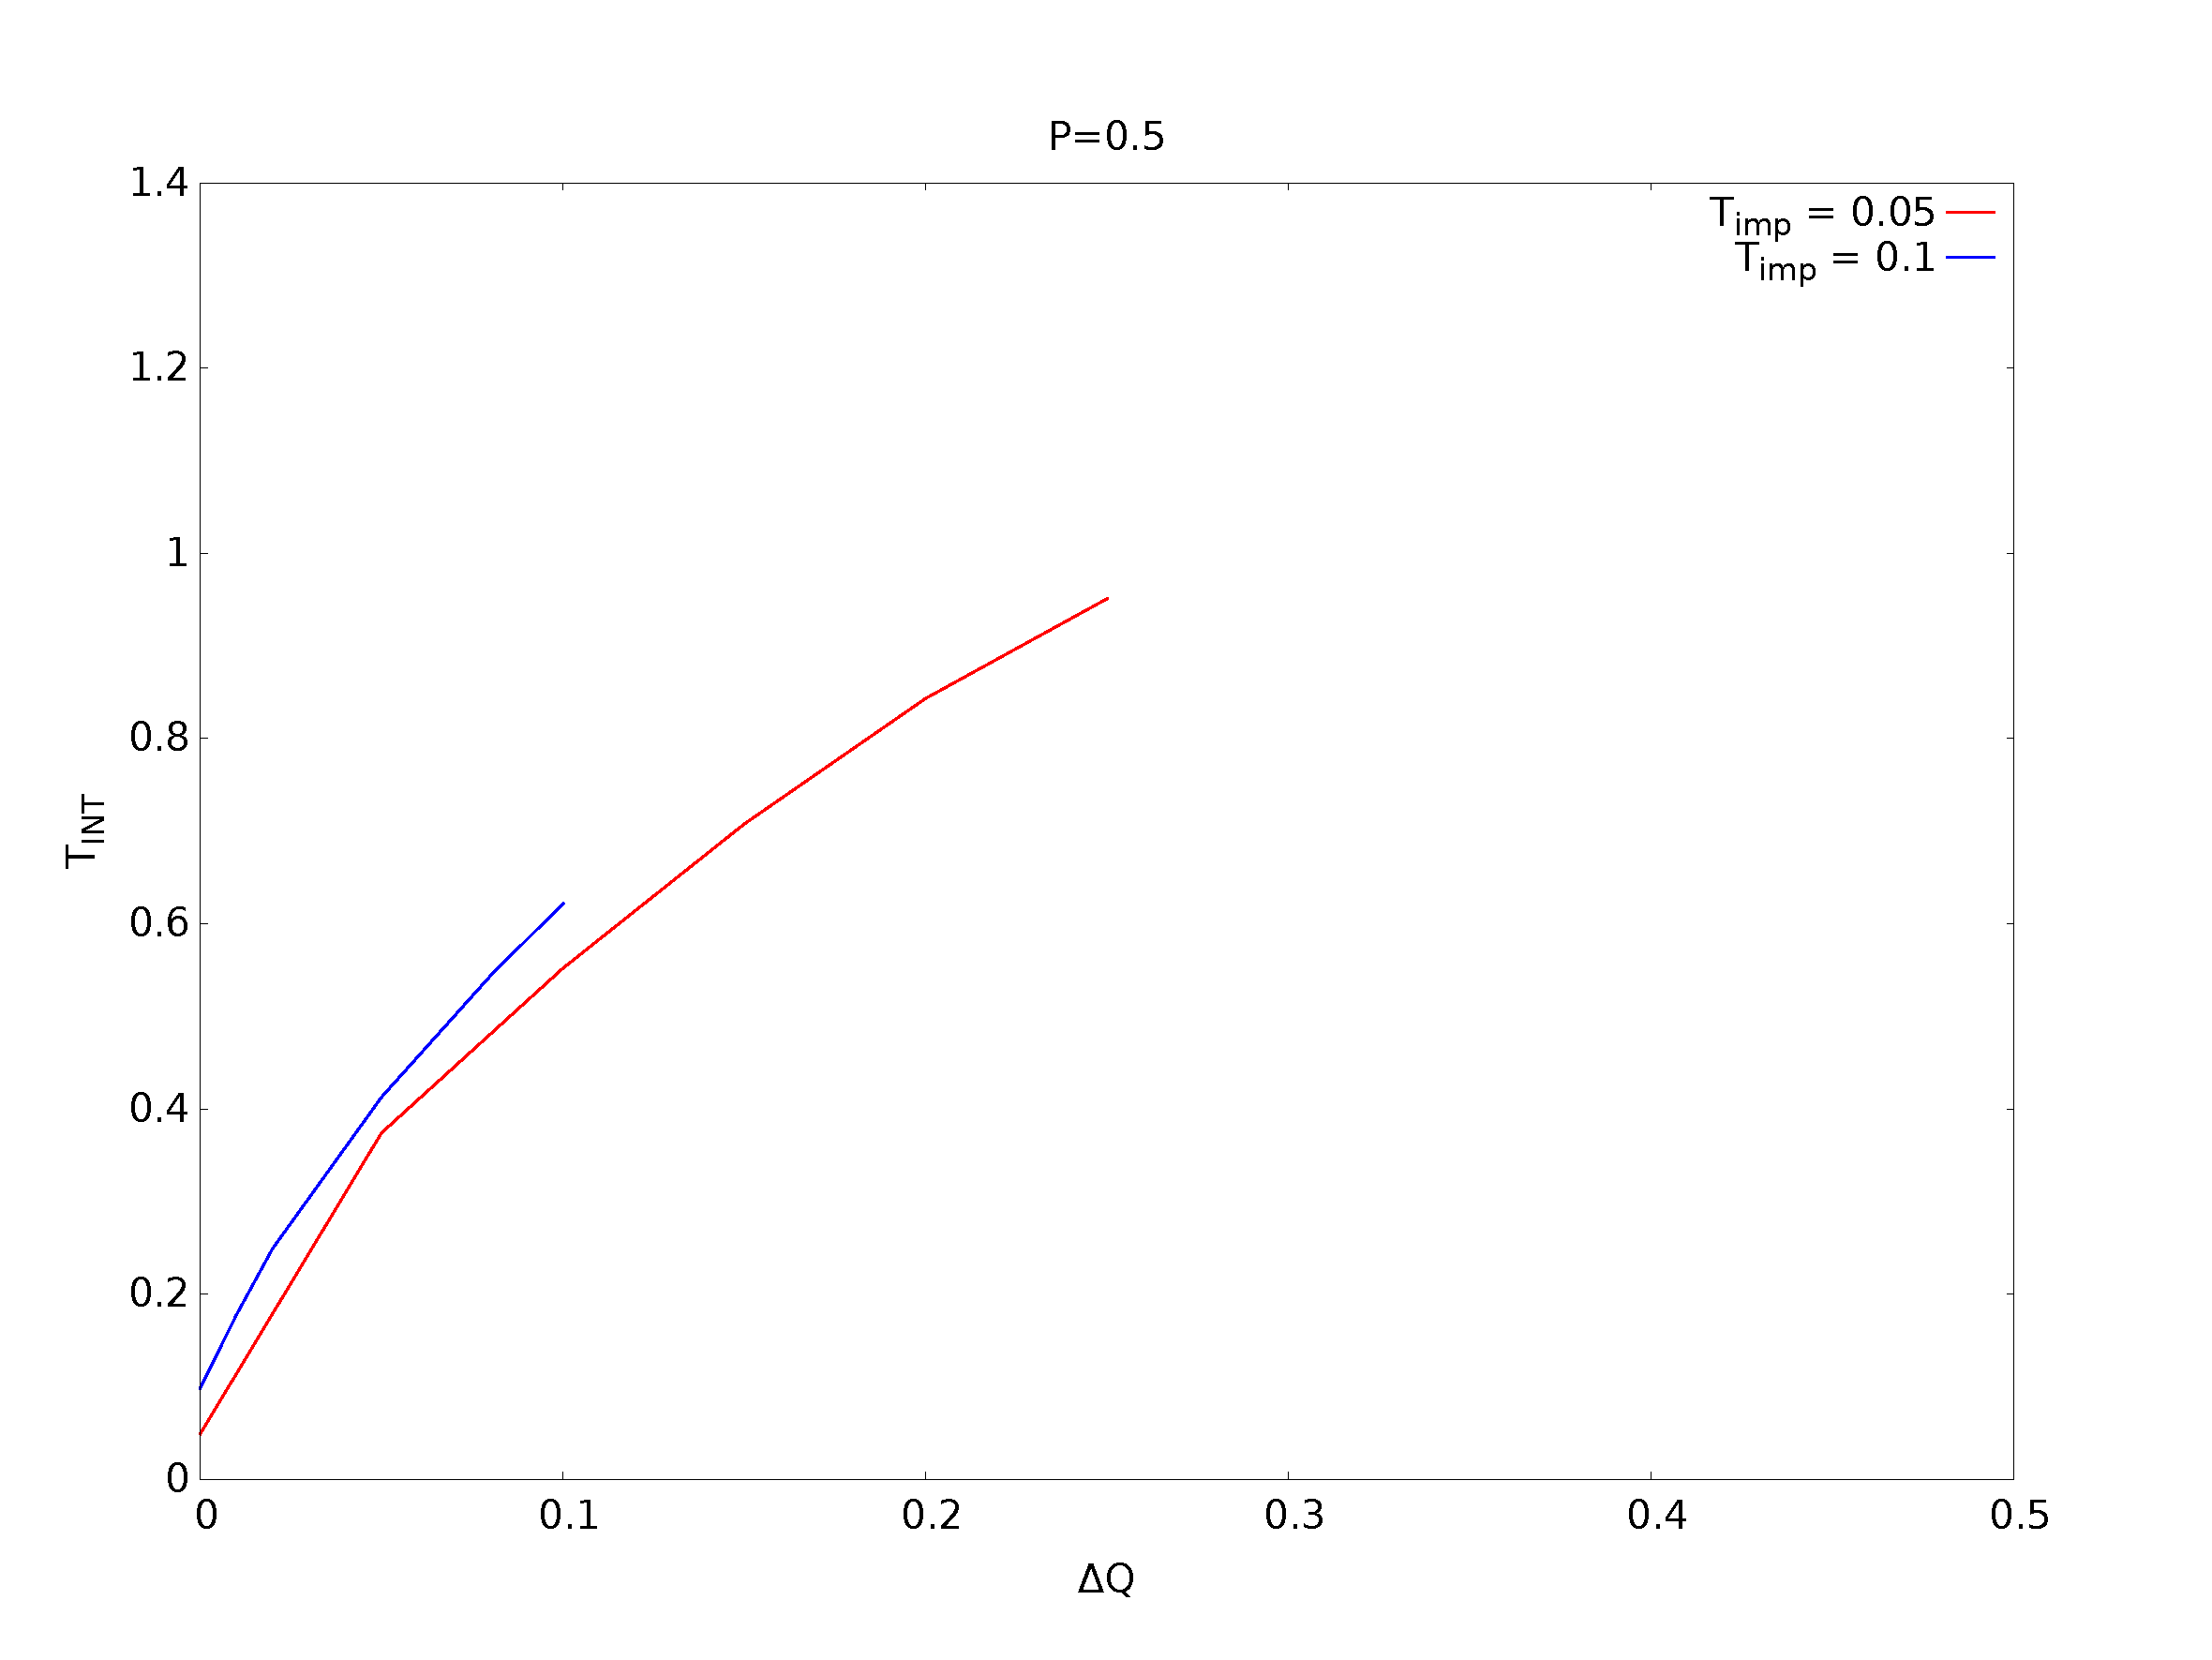
\includegraphics[scale=0.09]{../images/p05_int.pdf}
        \end{subfigure} 
        \
        \begin{subfigure}[t]{0.3\textwidth}
            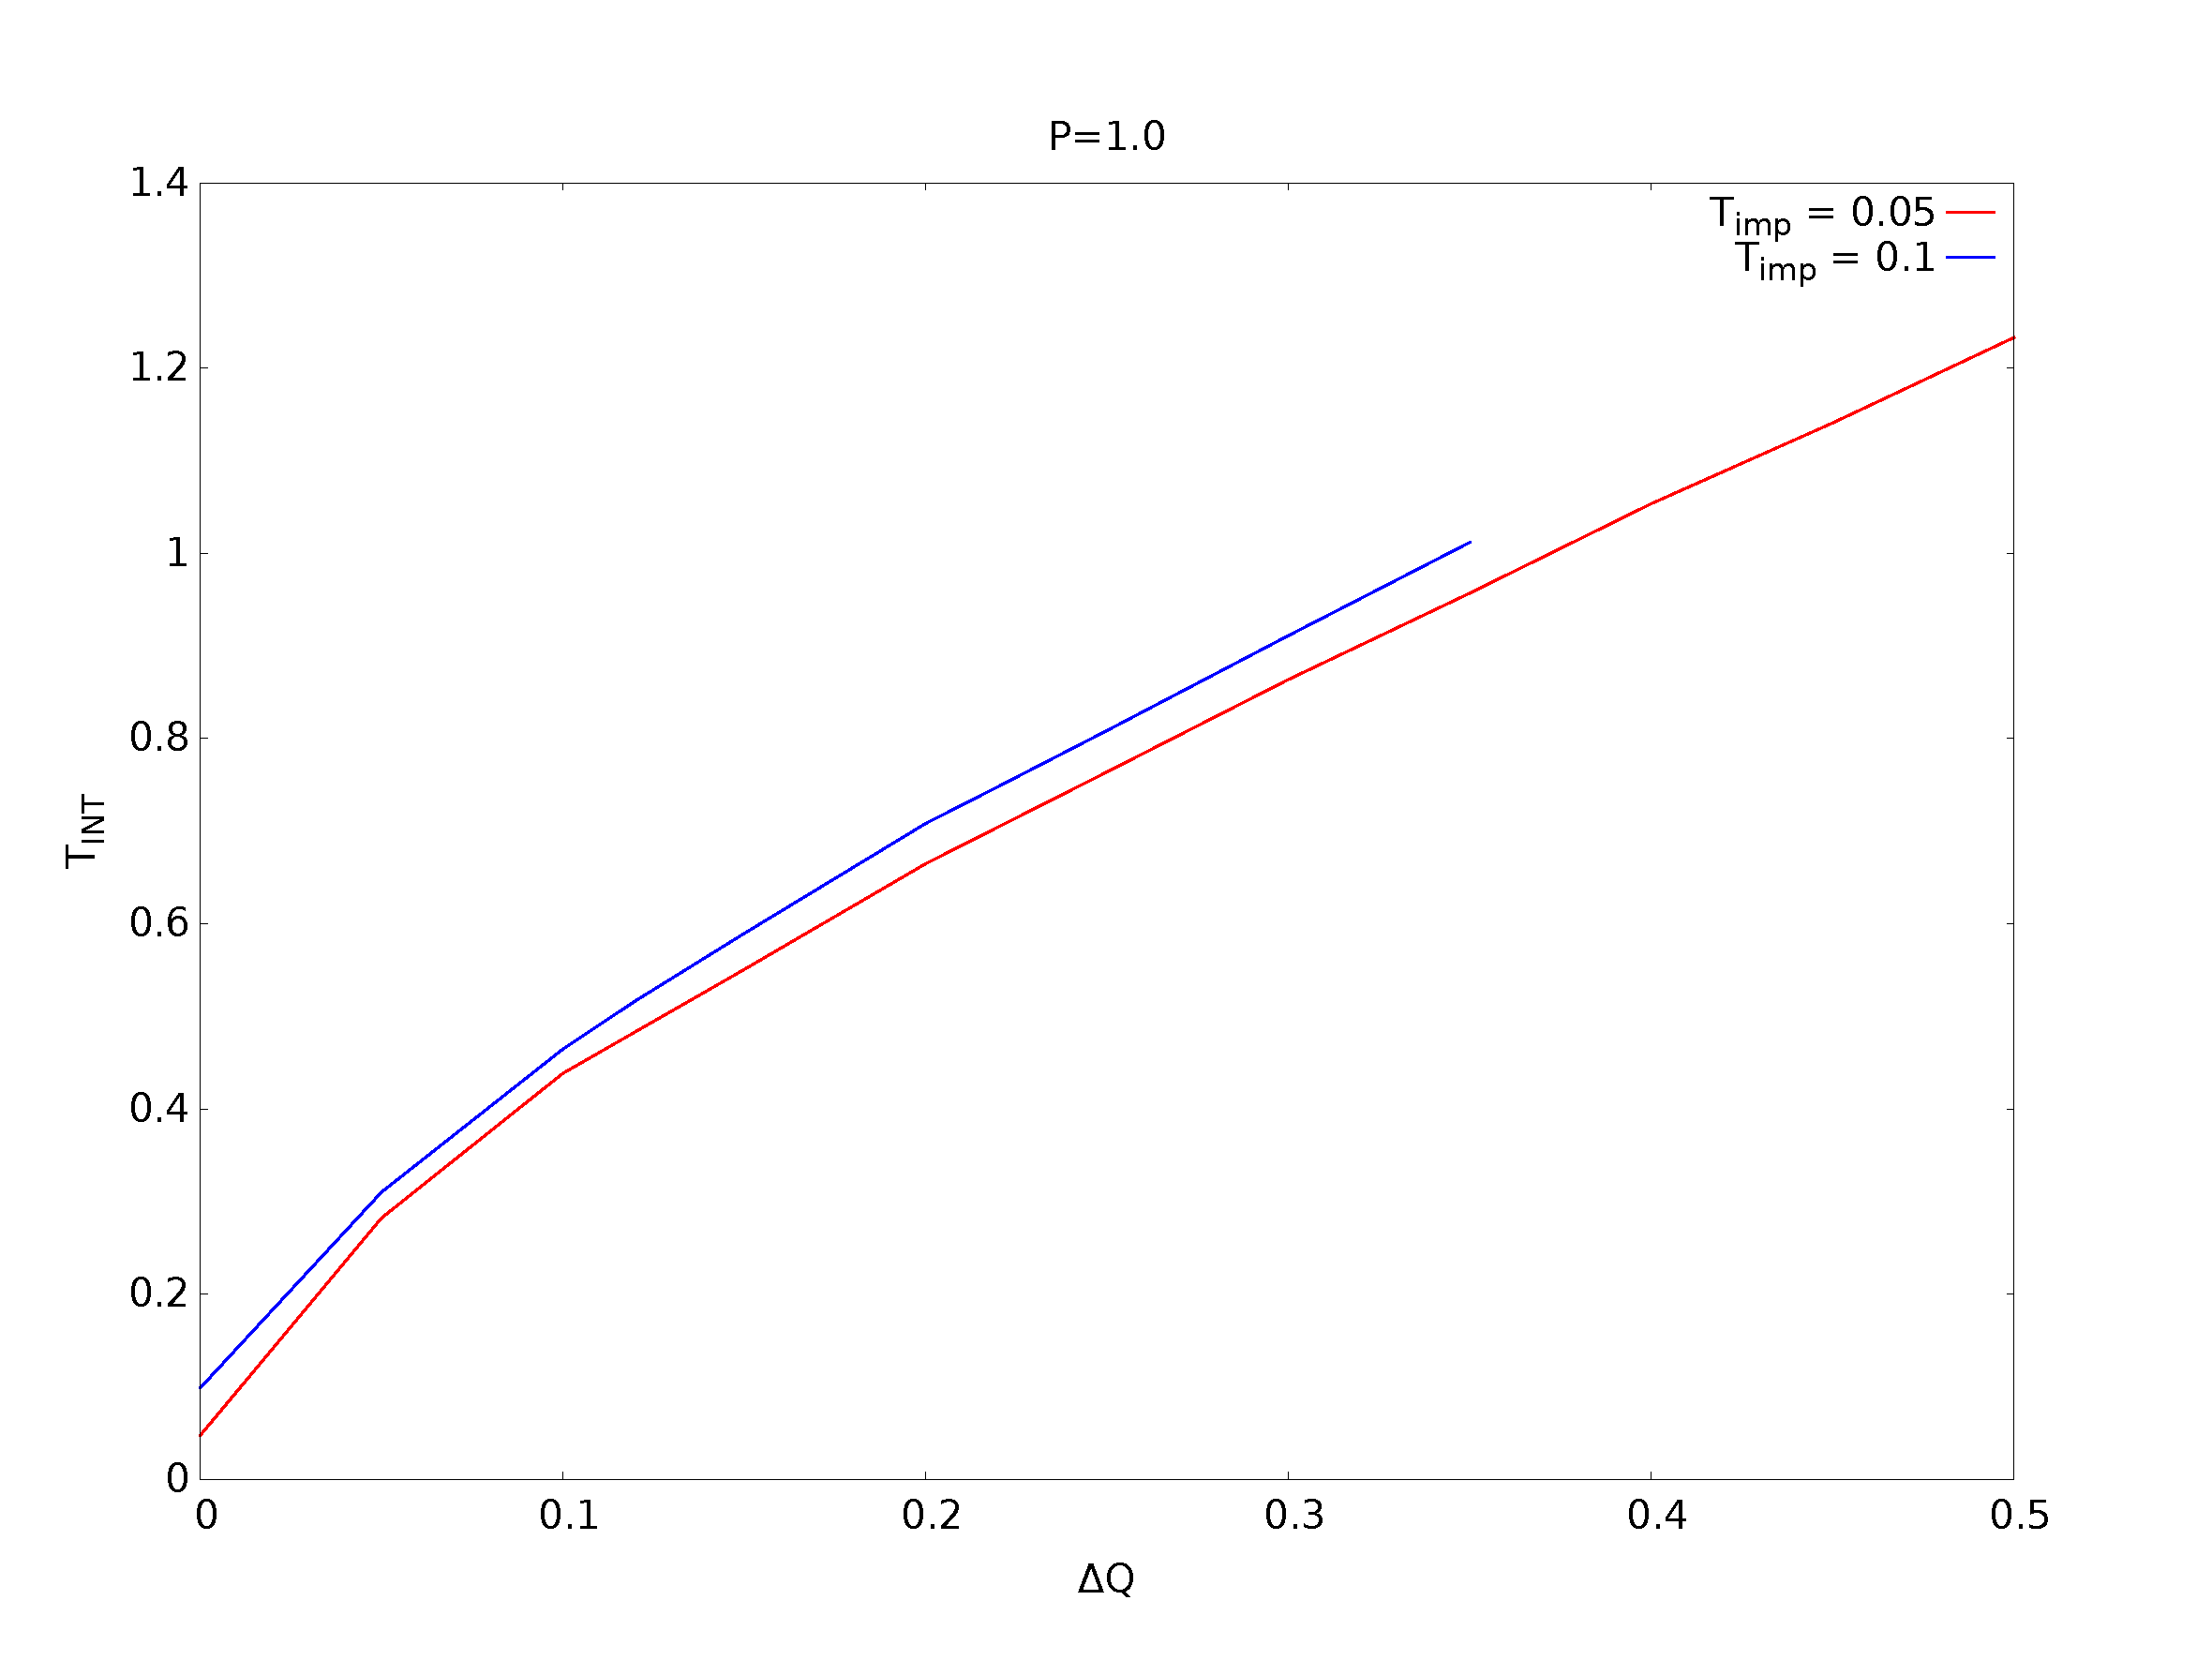
\includegraphics[scale=0.09]{../images/p1_int.pdf}
        \end{subfigure} 
        \\
        \begin{subfigure}[t]{0.3\textwidth}
            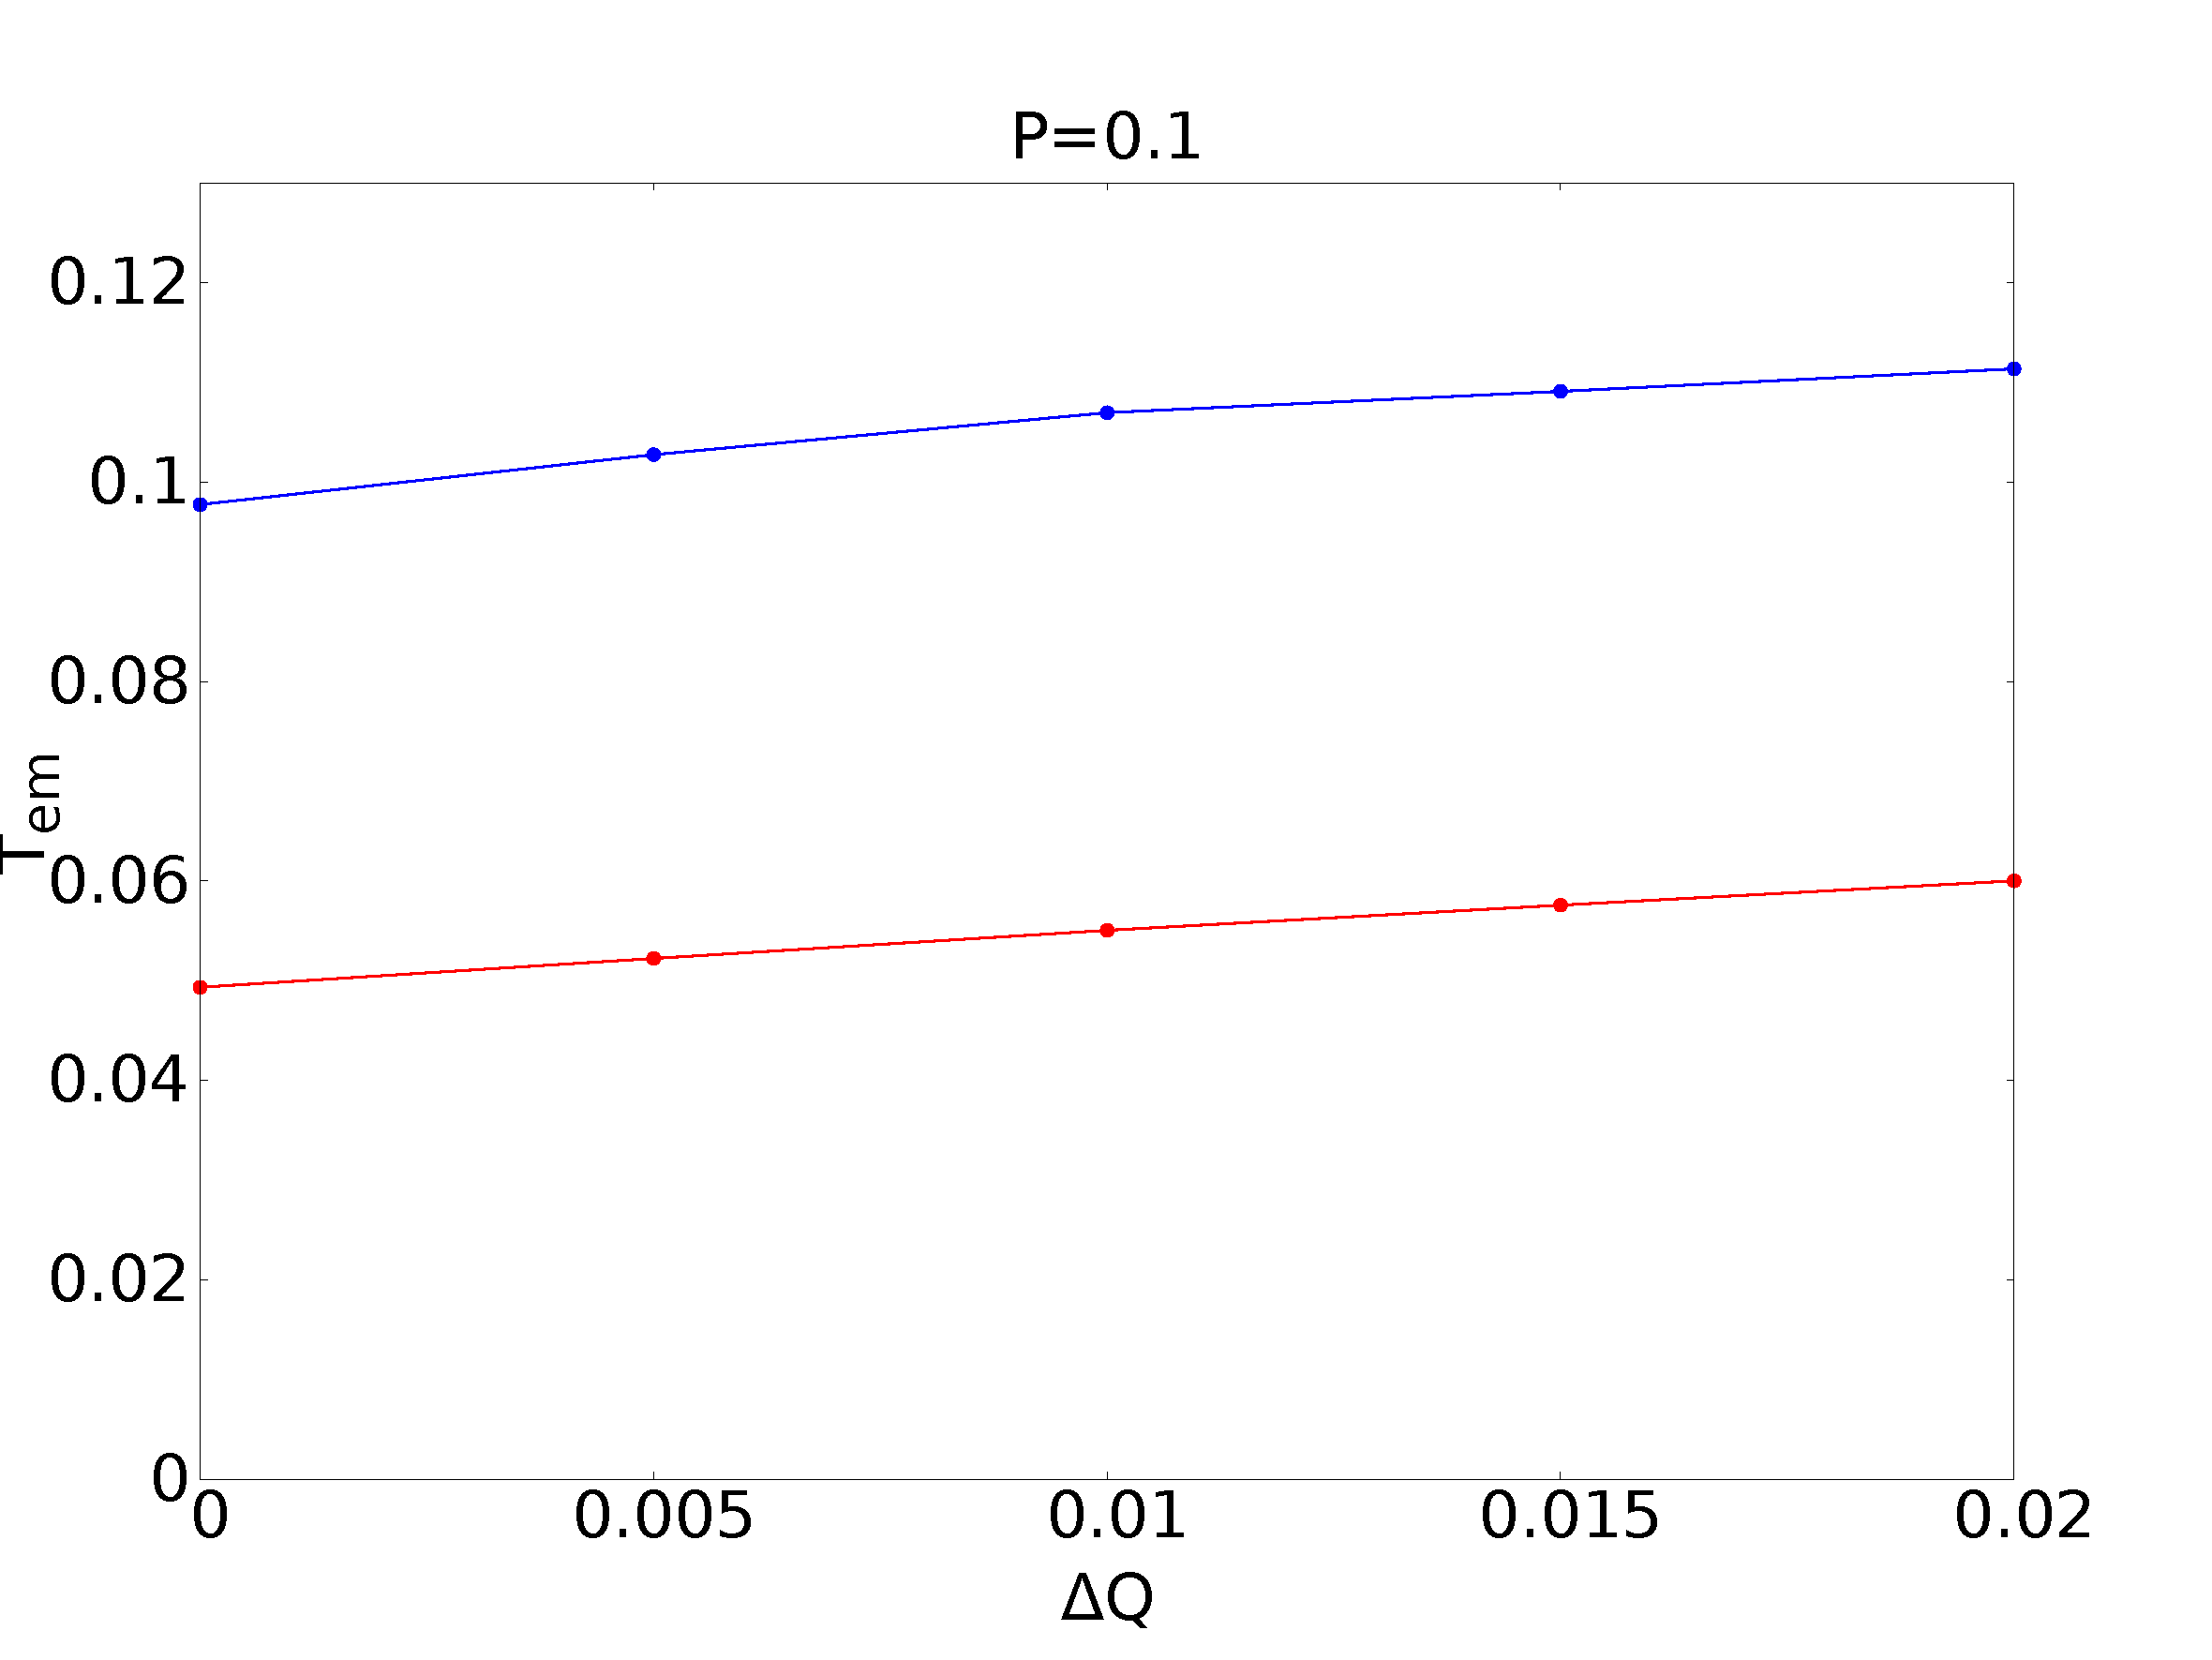
\includegraphics[scale=0.09]{../images/p01_out.pdf}
        \end{subfigure} 
        \
        \begin{subfigure}[t]{0.3\textwidth}
            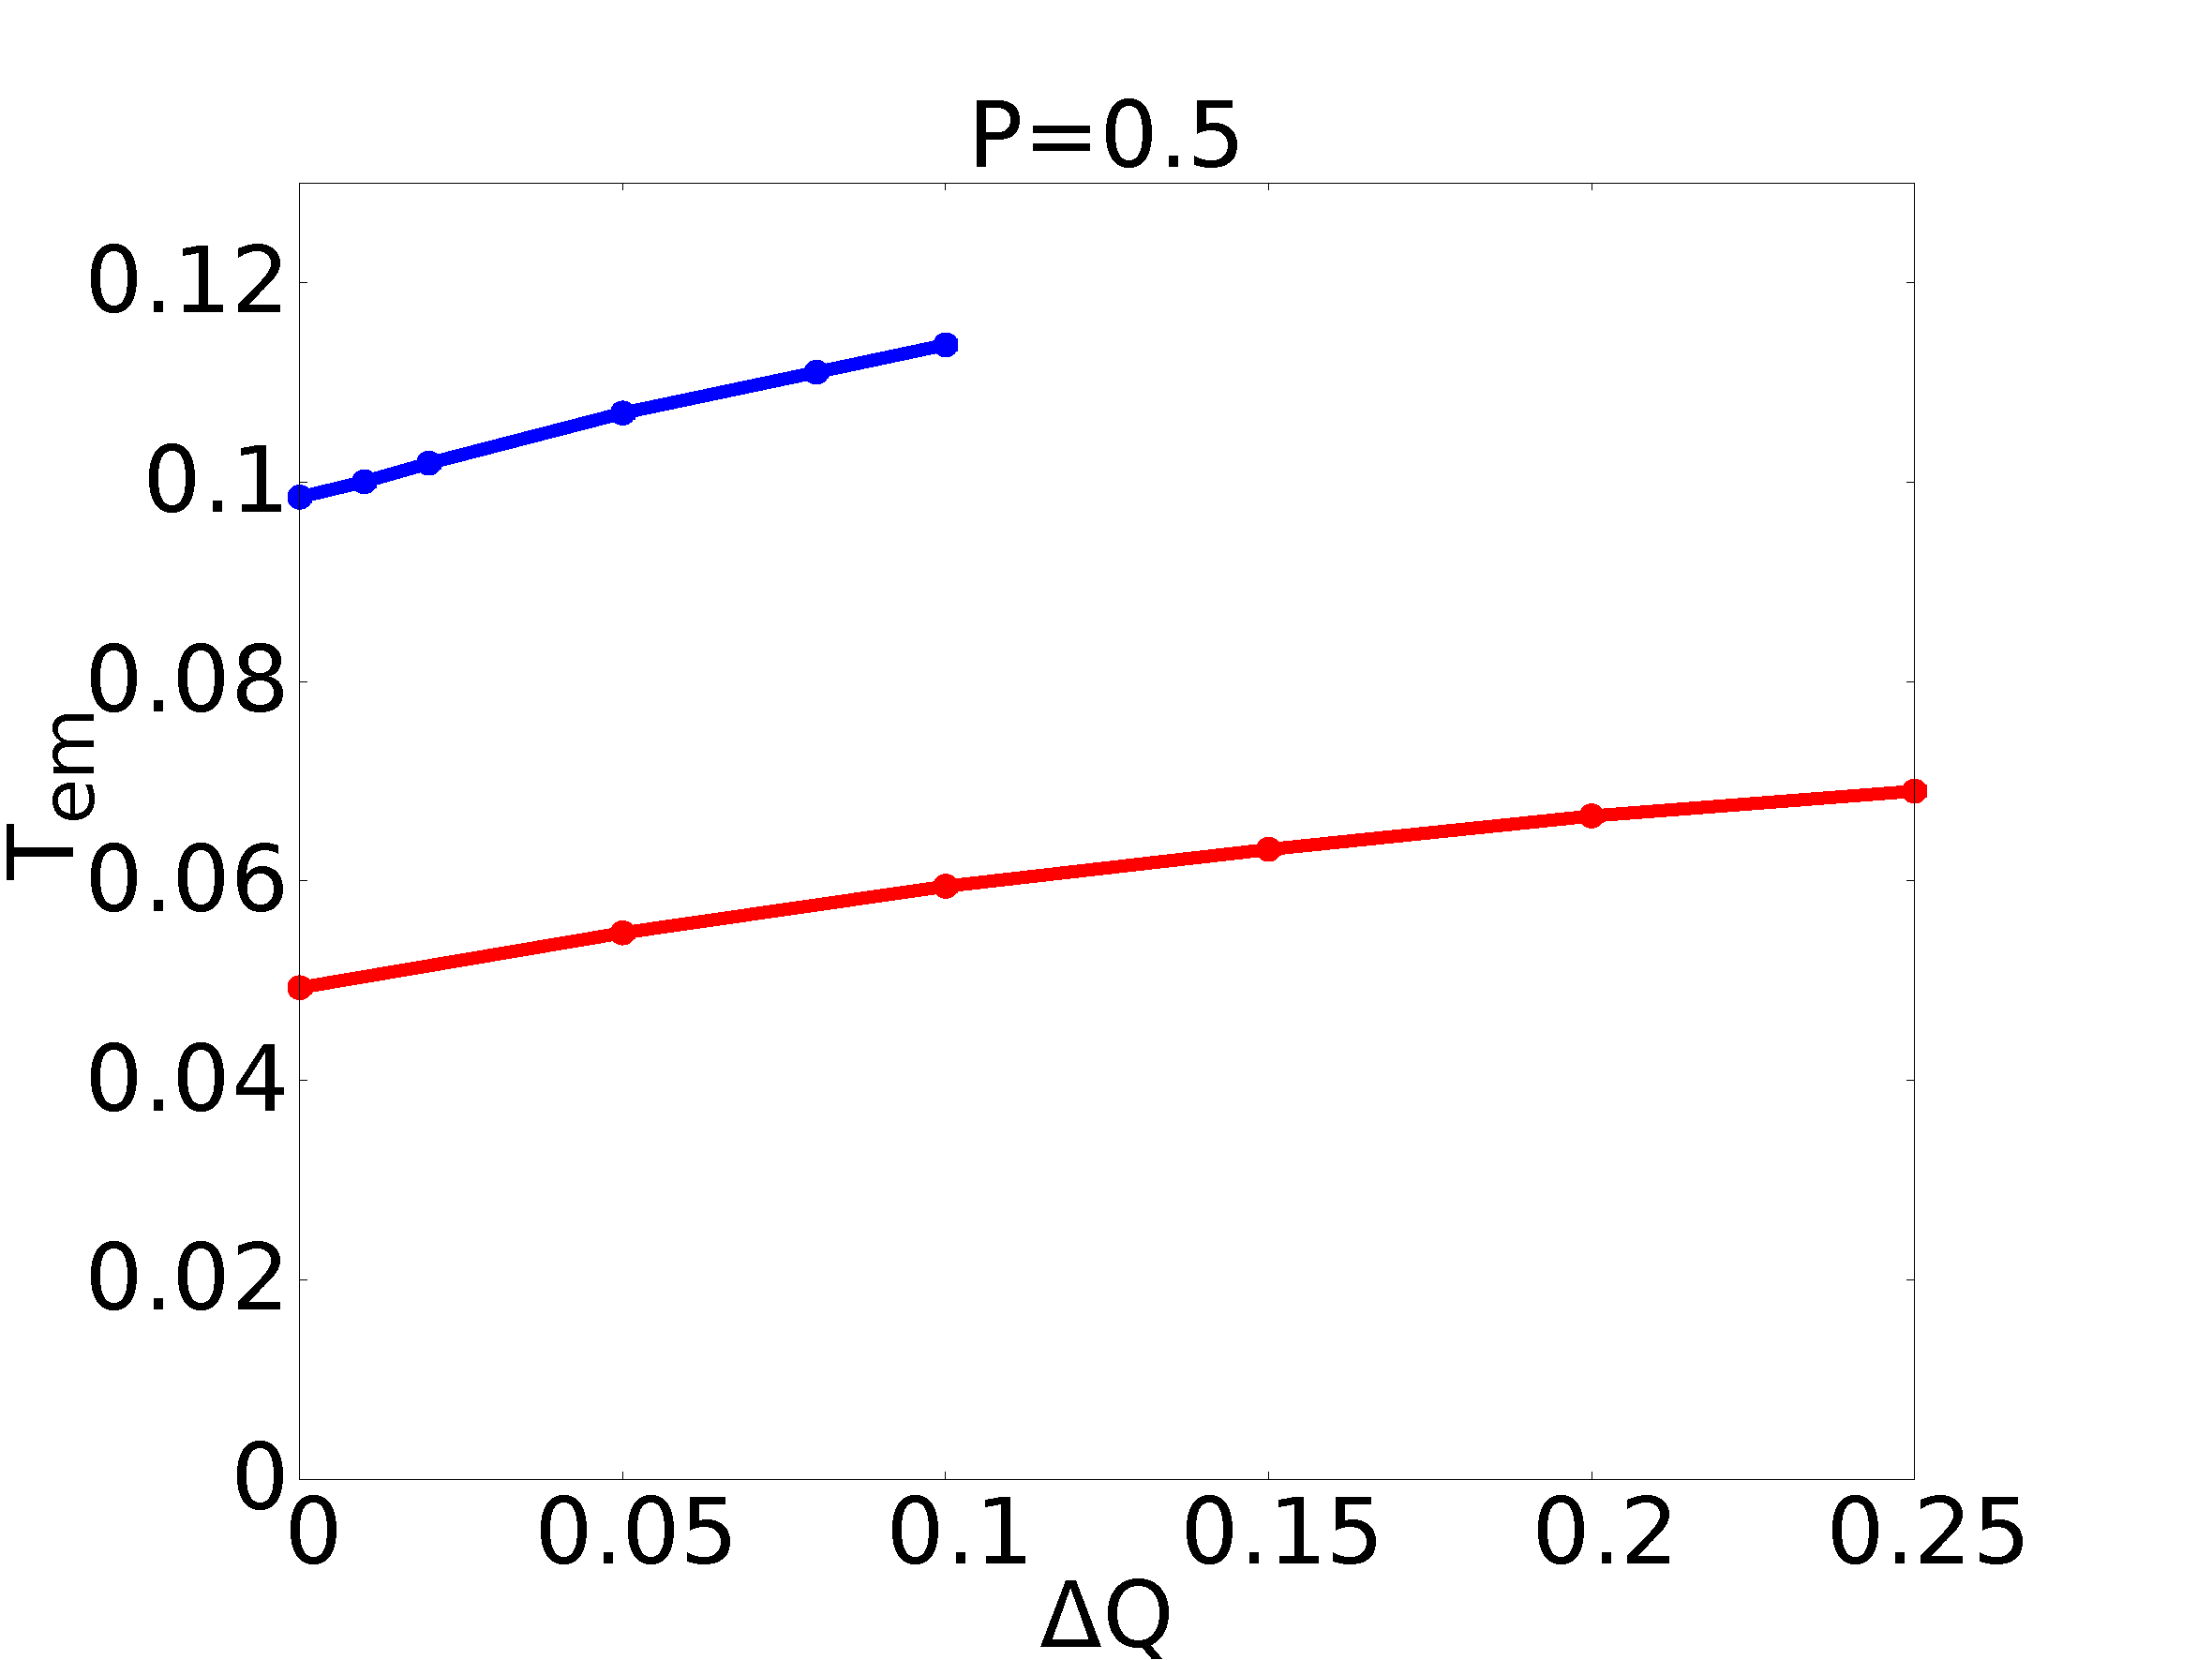
\includegraphics[scale=0.09]{../images/p05_out.pdf}
        \end{subfigure} 
        \
        \begin{subfigure}[t]{0.3\textwidth}
            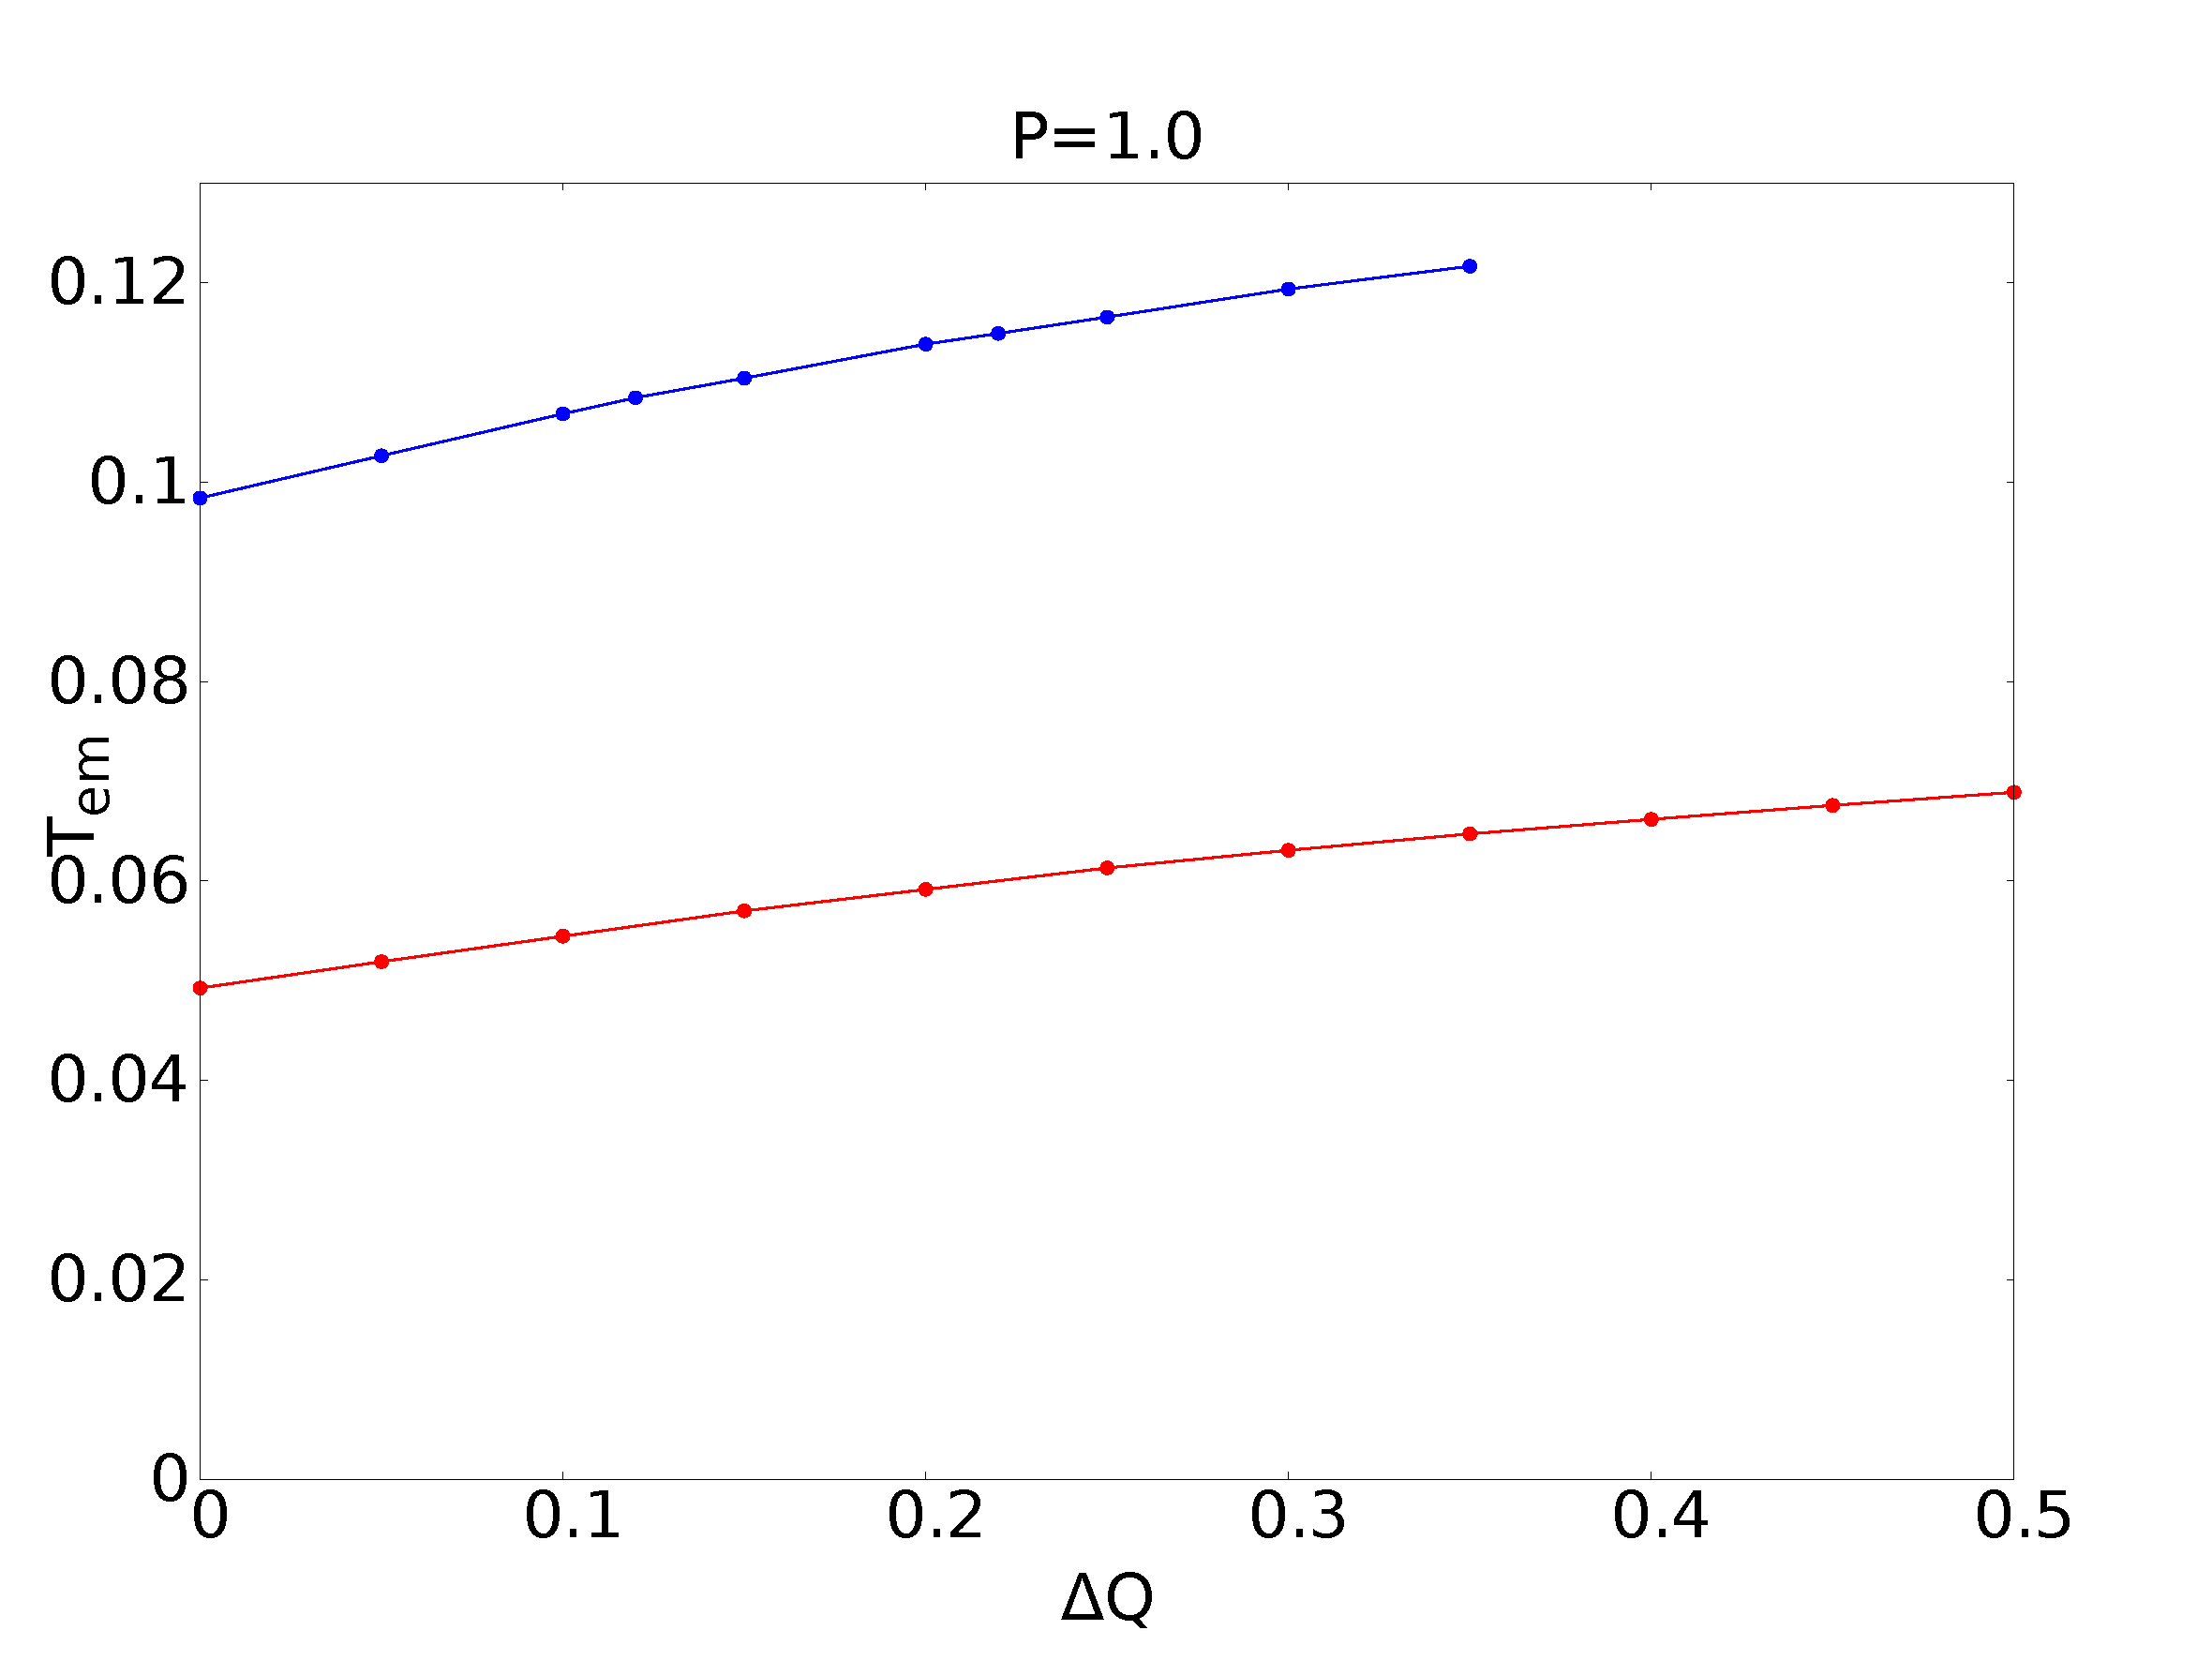
\includegraphics[scale=0.09]{../images/p1_out.pdf}
        \end{subfigure} 
    \end{center}
\end{figure}
\end{frame}

\begin{frame}
\frametitle{Ergebnisse -- Schwerpunktsbewegung}
\begin{figure}
    \begin{center}
        \begin{subfigure}[t]{0.3\textwidth}
            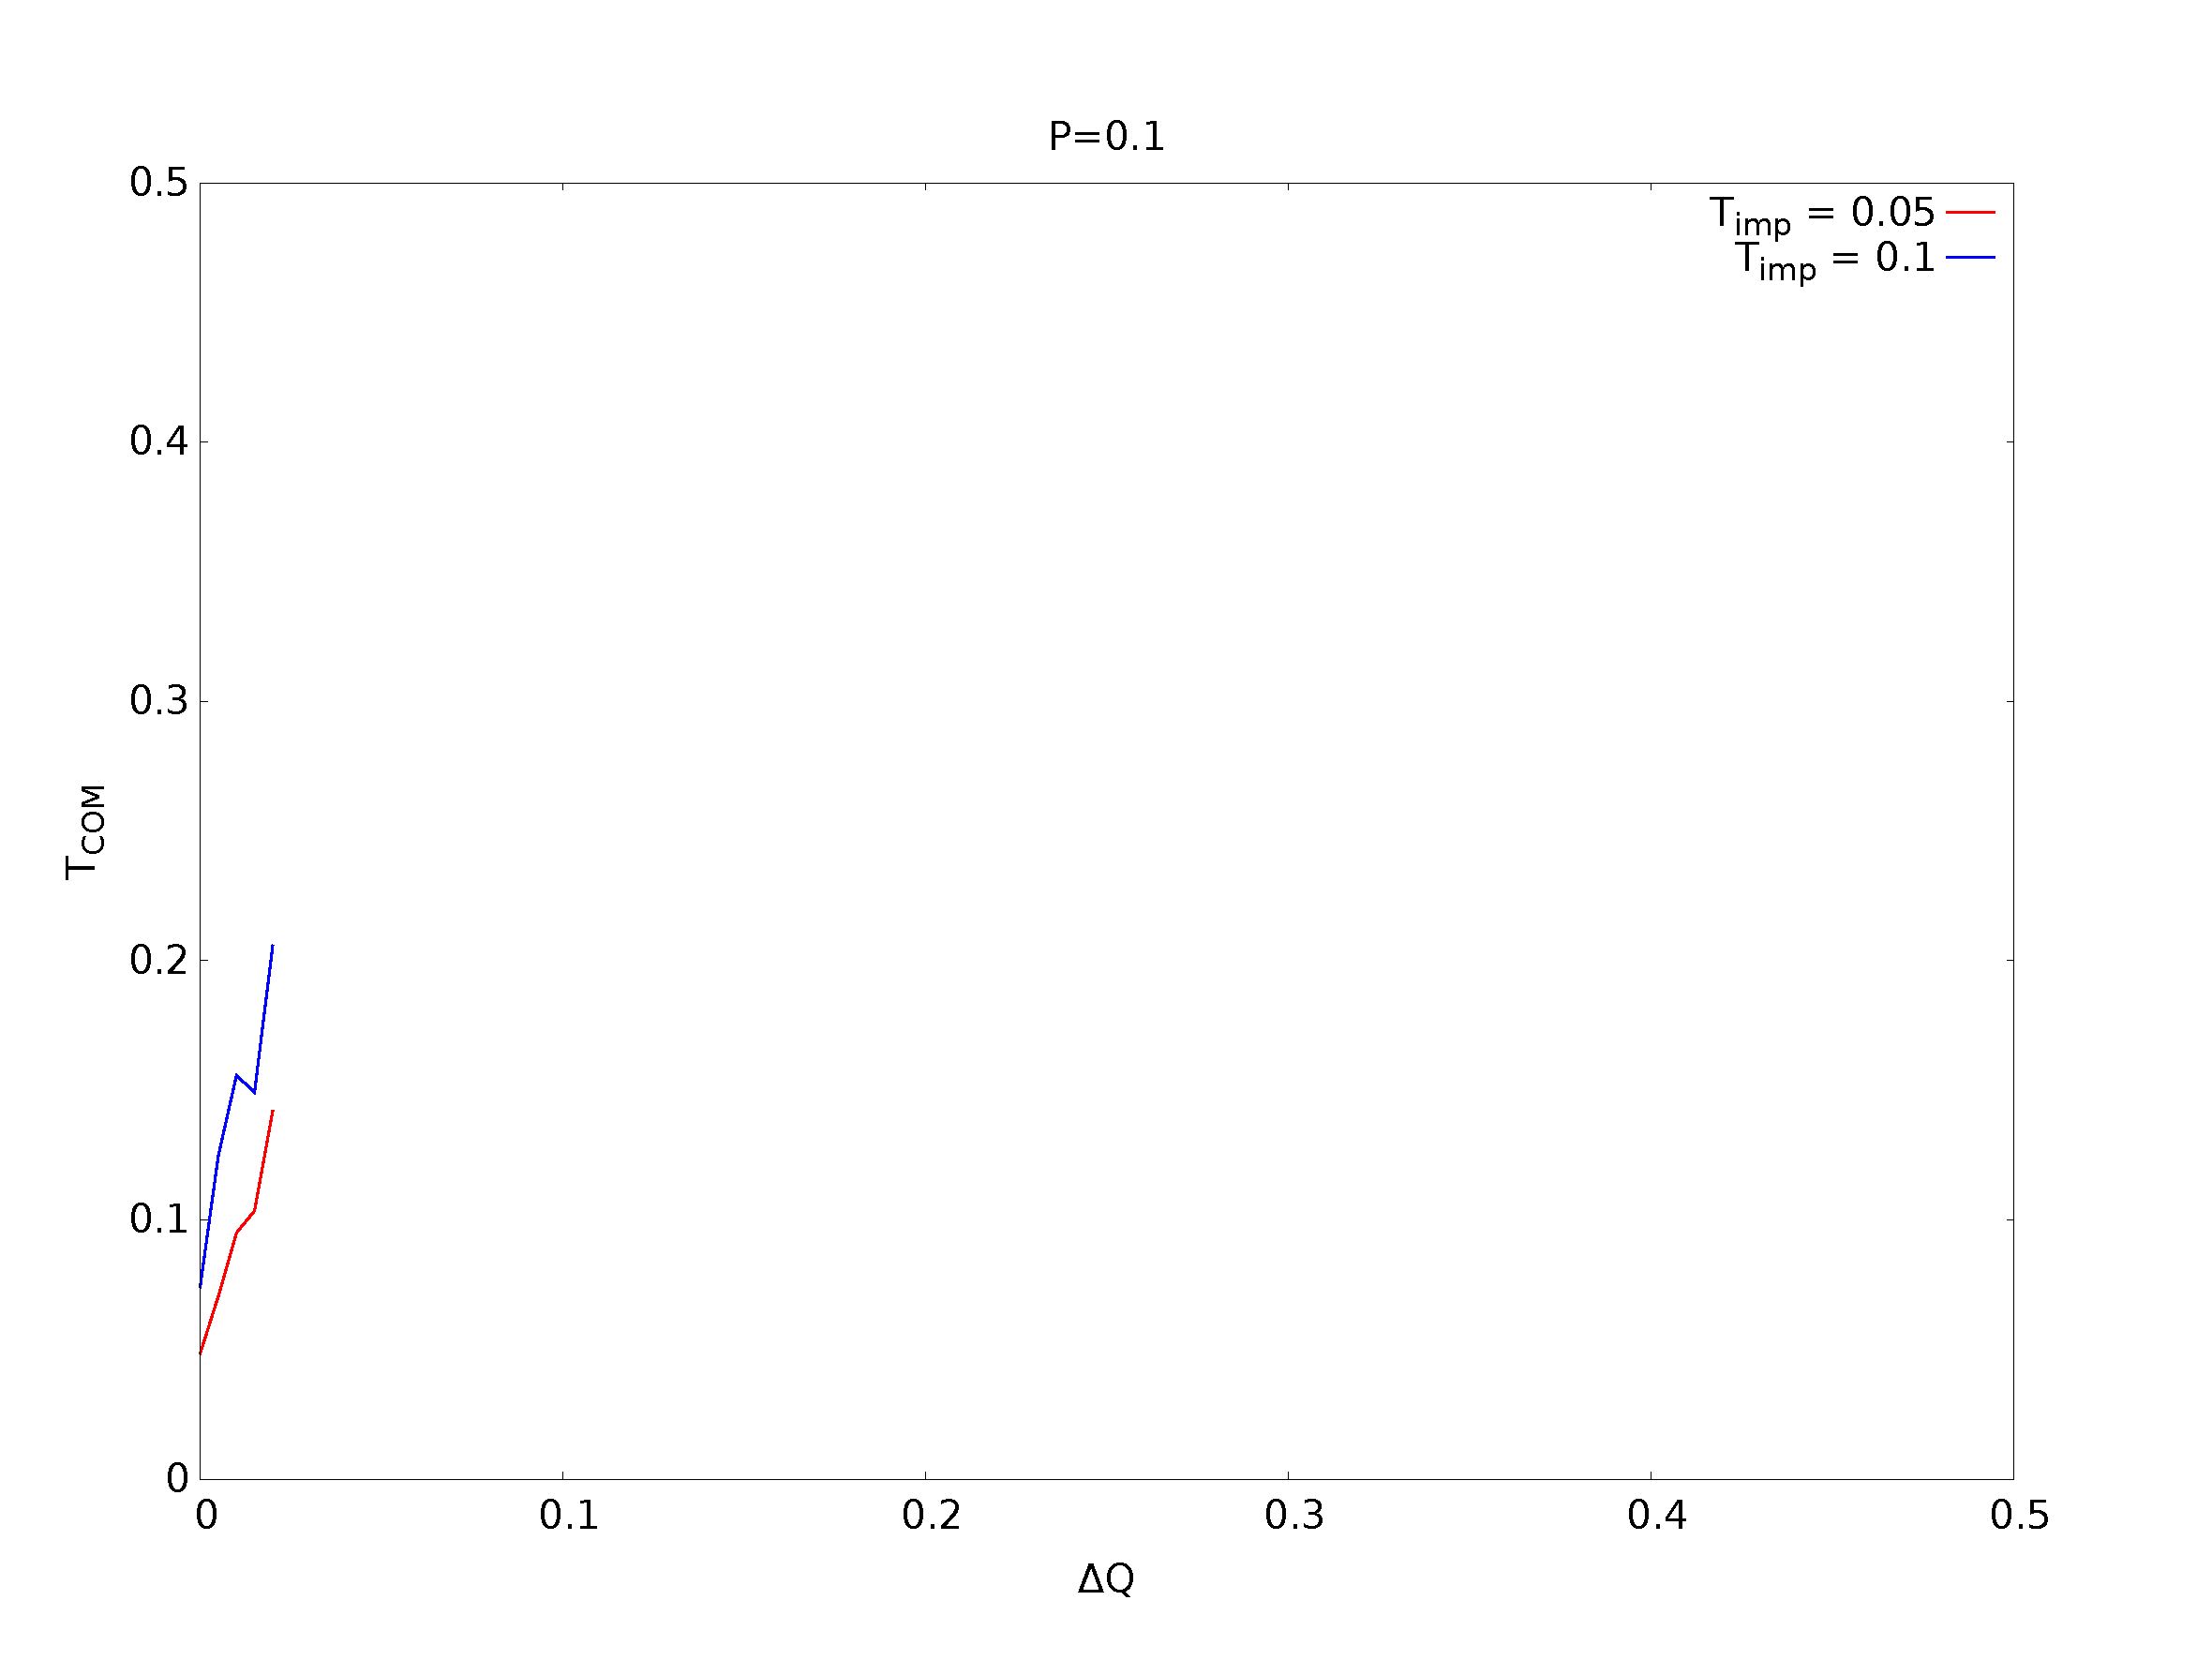
\includegraphics[scale=0.11]{../images/p01_com.pdf}
        \end{subfigure} 
        \
        \begin{subfigure}[t]{0.3\textwidth}
            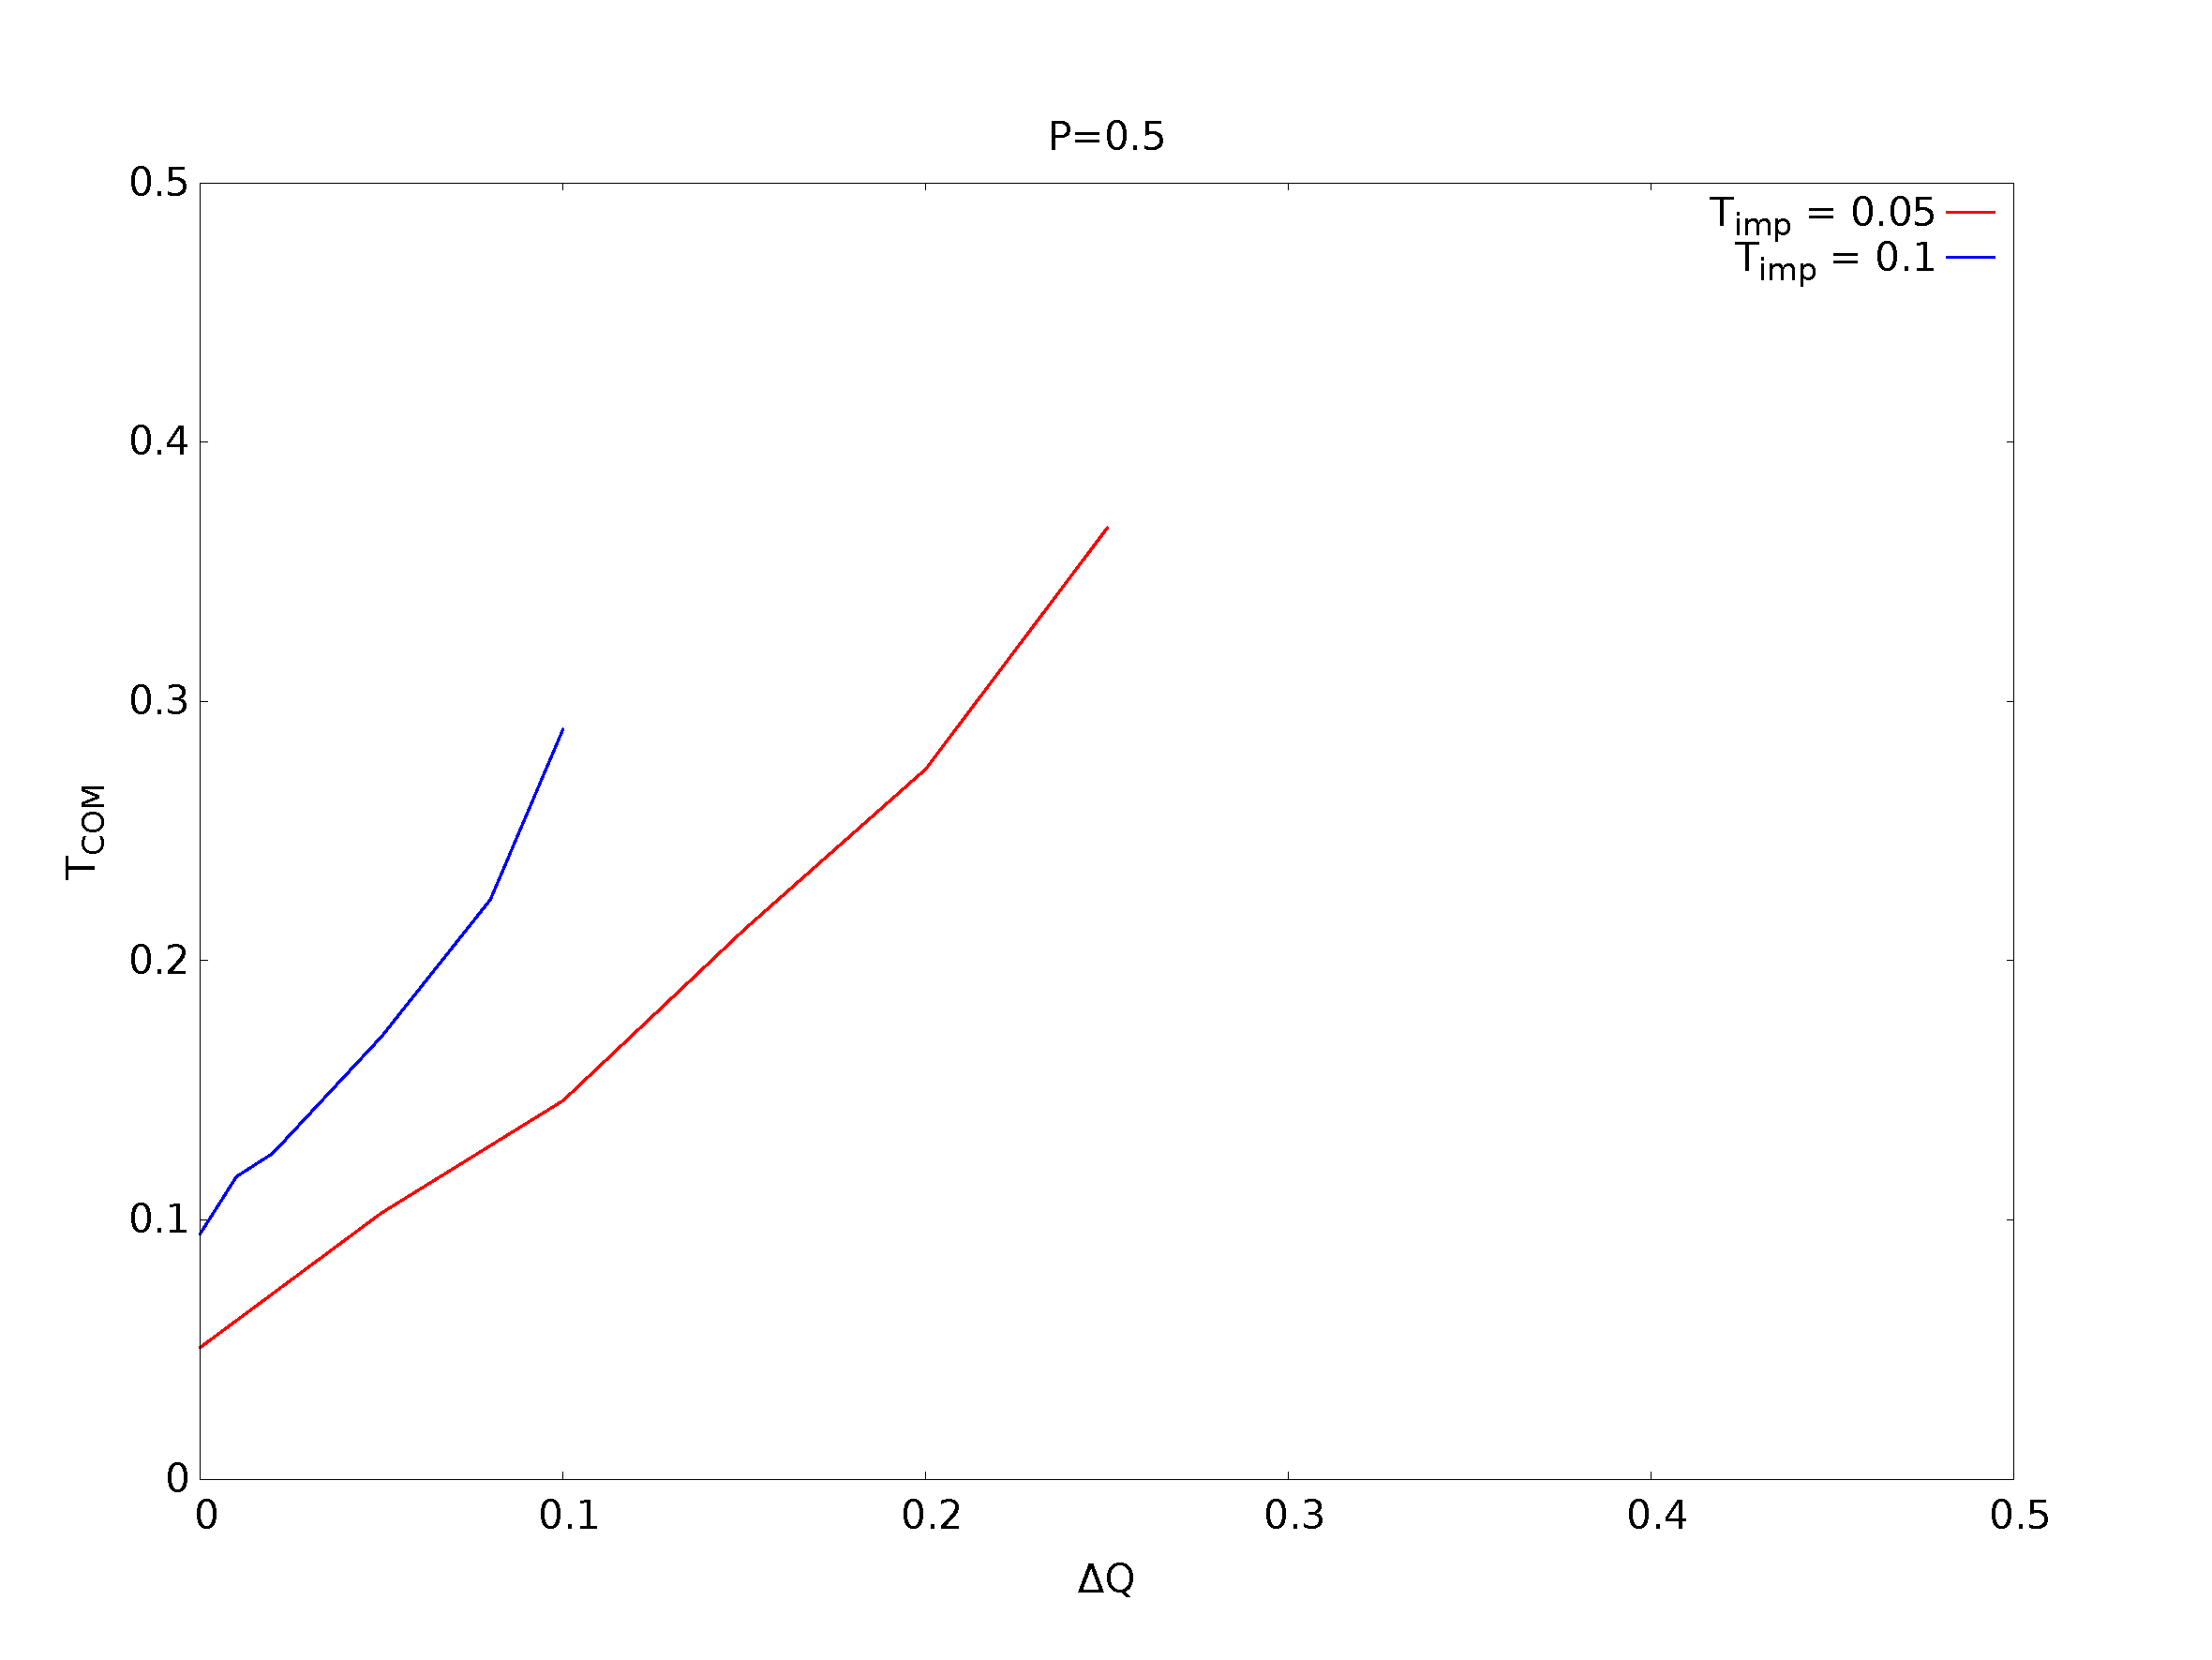
\includegraphics[scale=0.11]{../images/p05_com.pdf}
        \end{subfigure} 
        \
        \begin{subfigure}[t]{0.3\textwidth}
            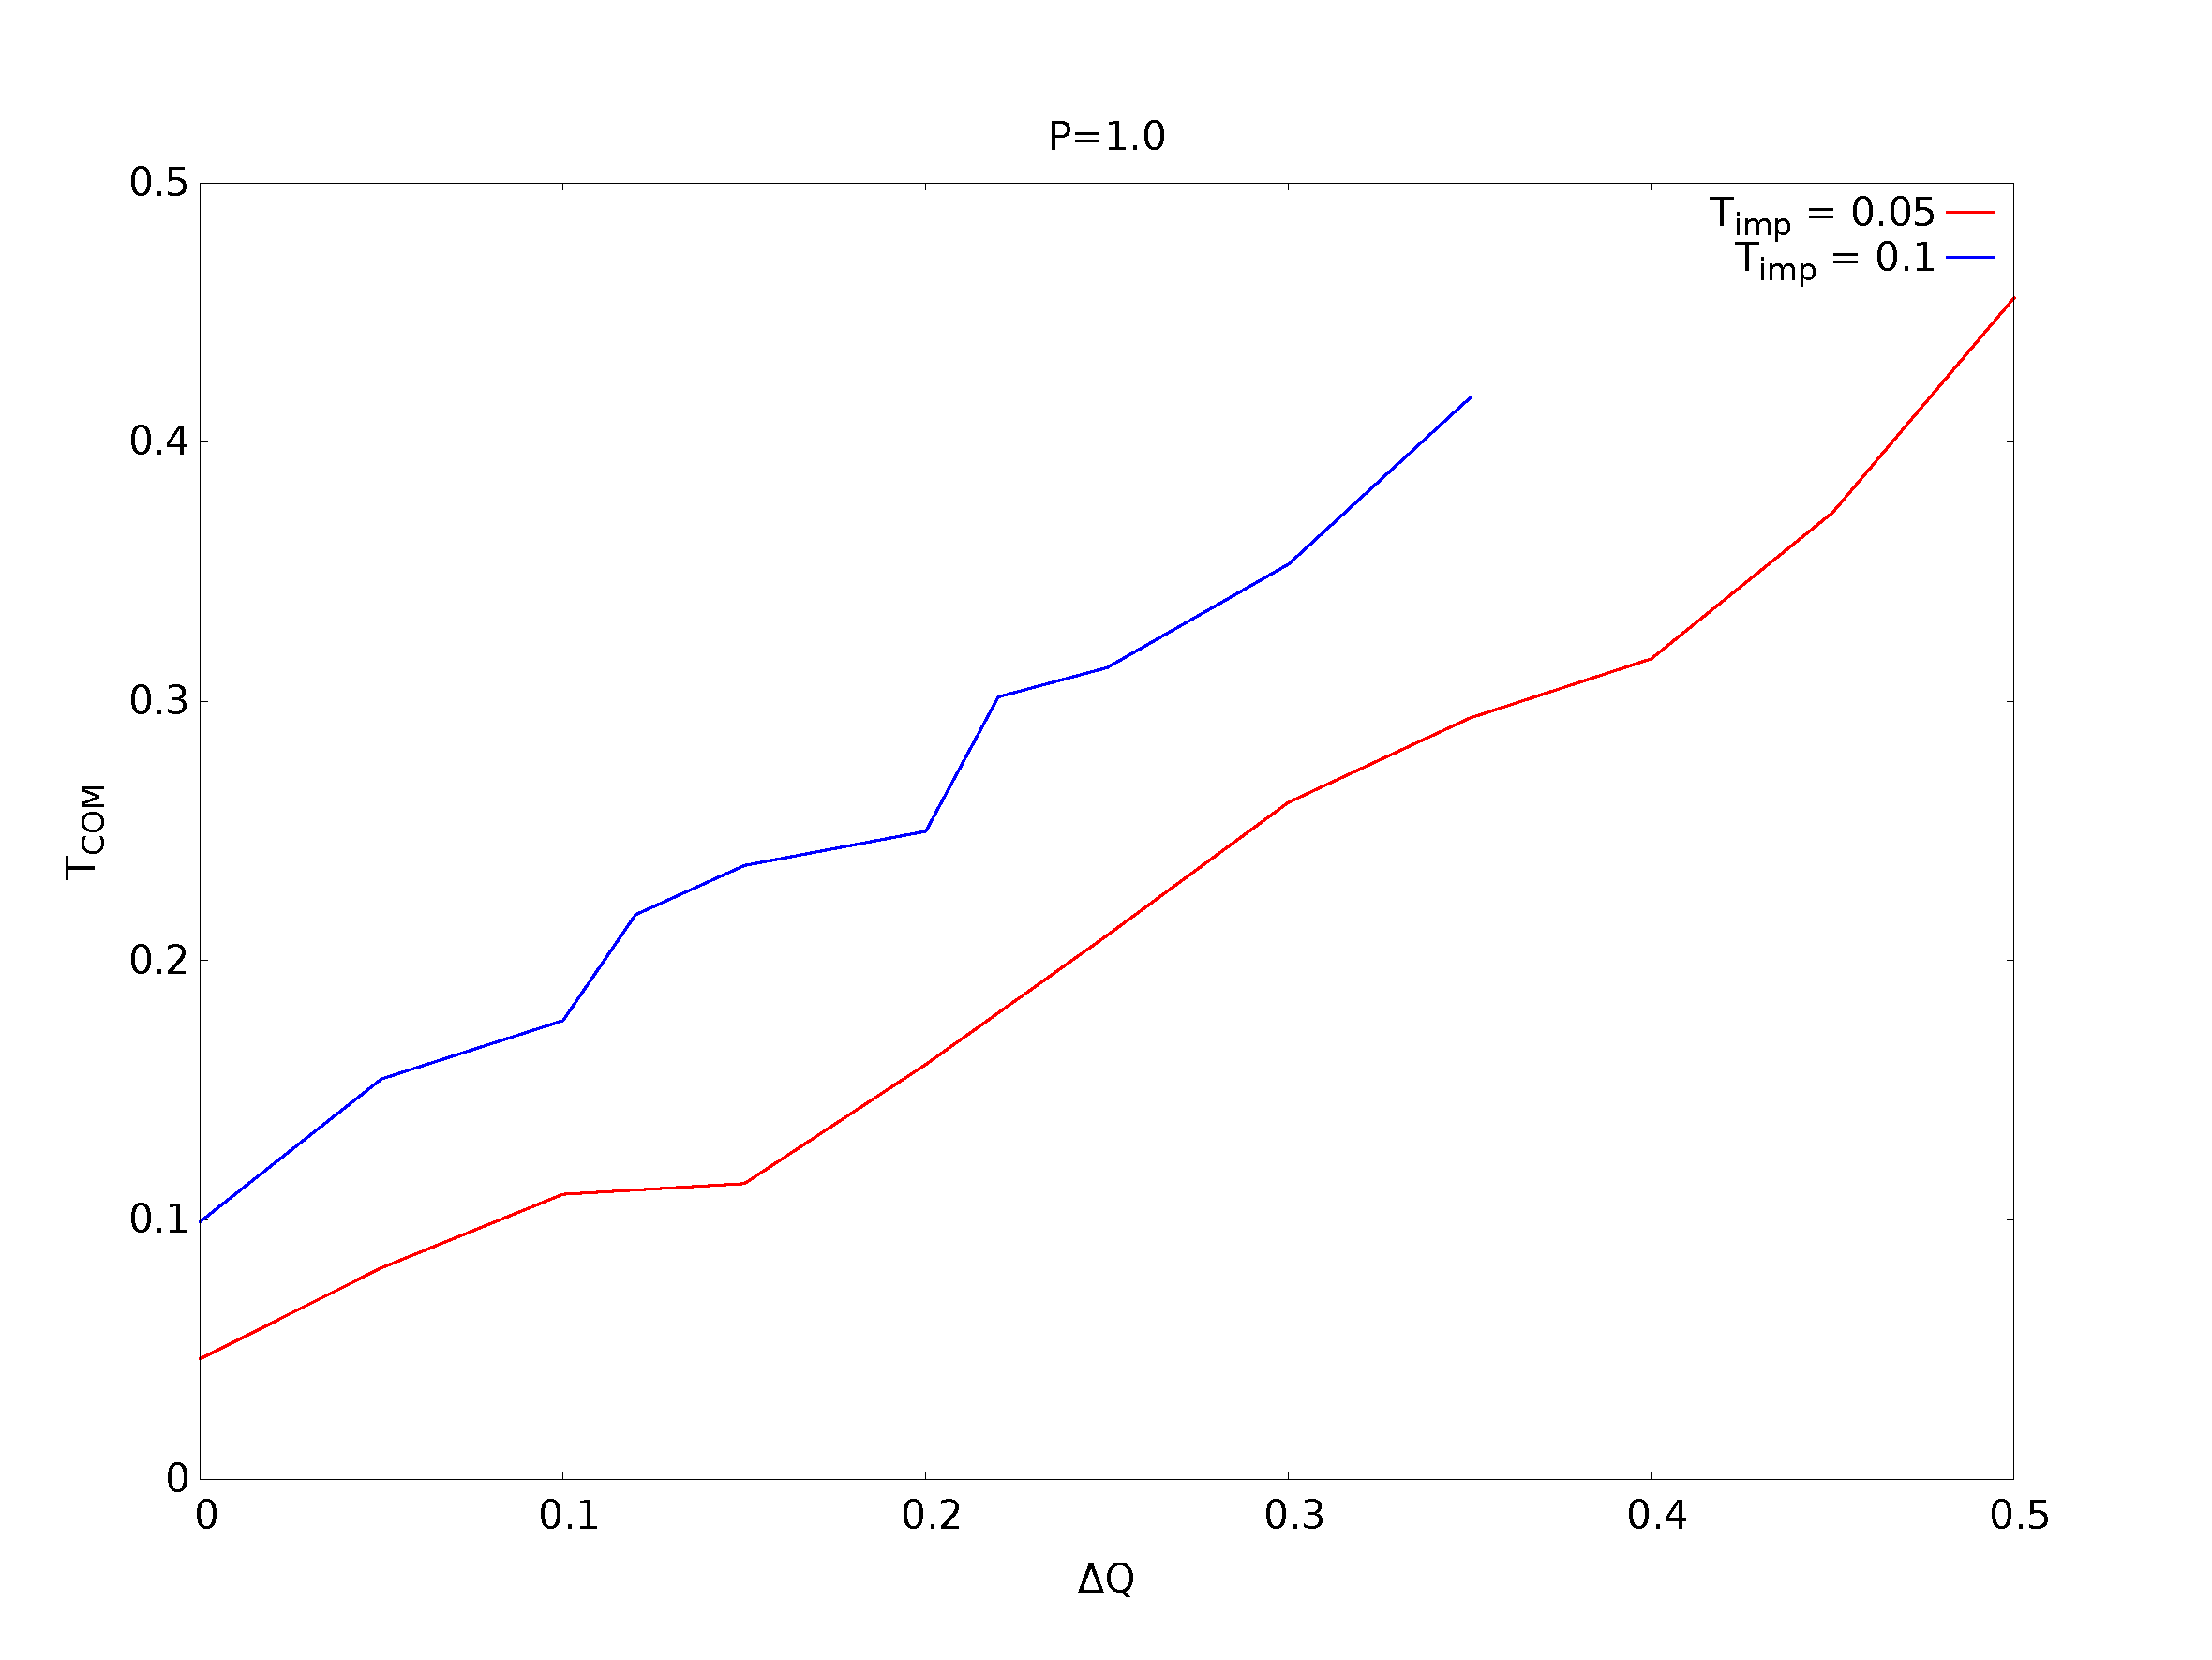
\includegraphics[scale=0.11]{../images/p1_com.pdf}
        \end{subfigure} 
    \end{center}
\end{figure}

\end{frame}

\begin{frame}
\frametitle{Ergebnisse -- Interne Temperatur}
\begin{figure}
    \begin{center}
        \begin{subfigure}[t]{0.3\textwidth}
            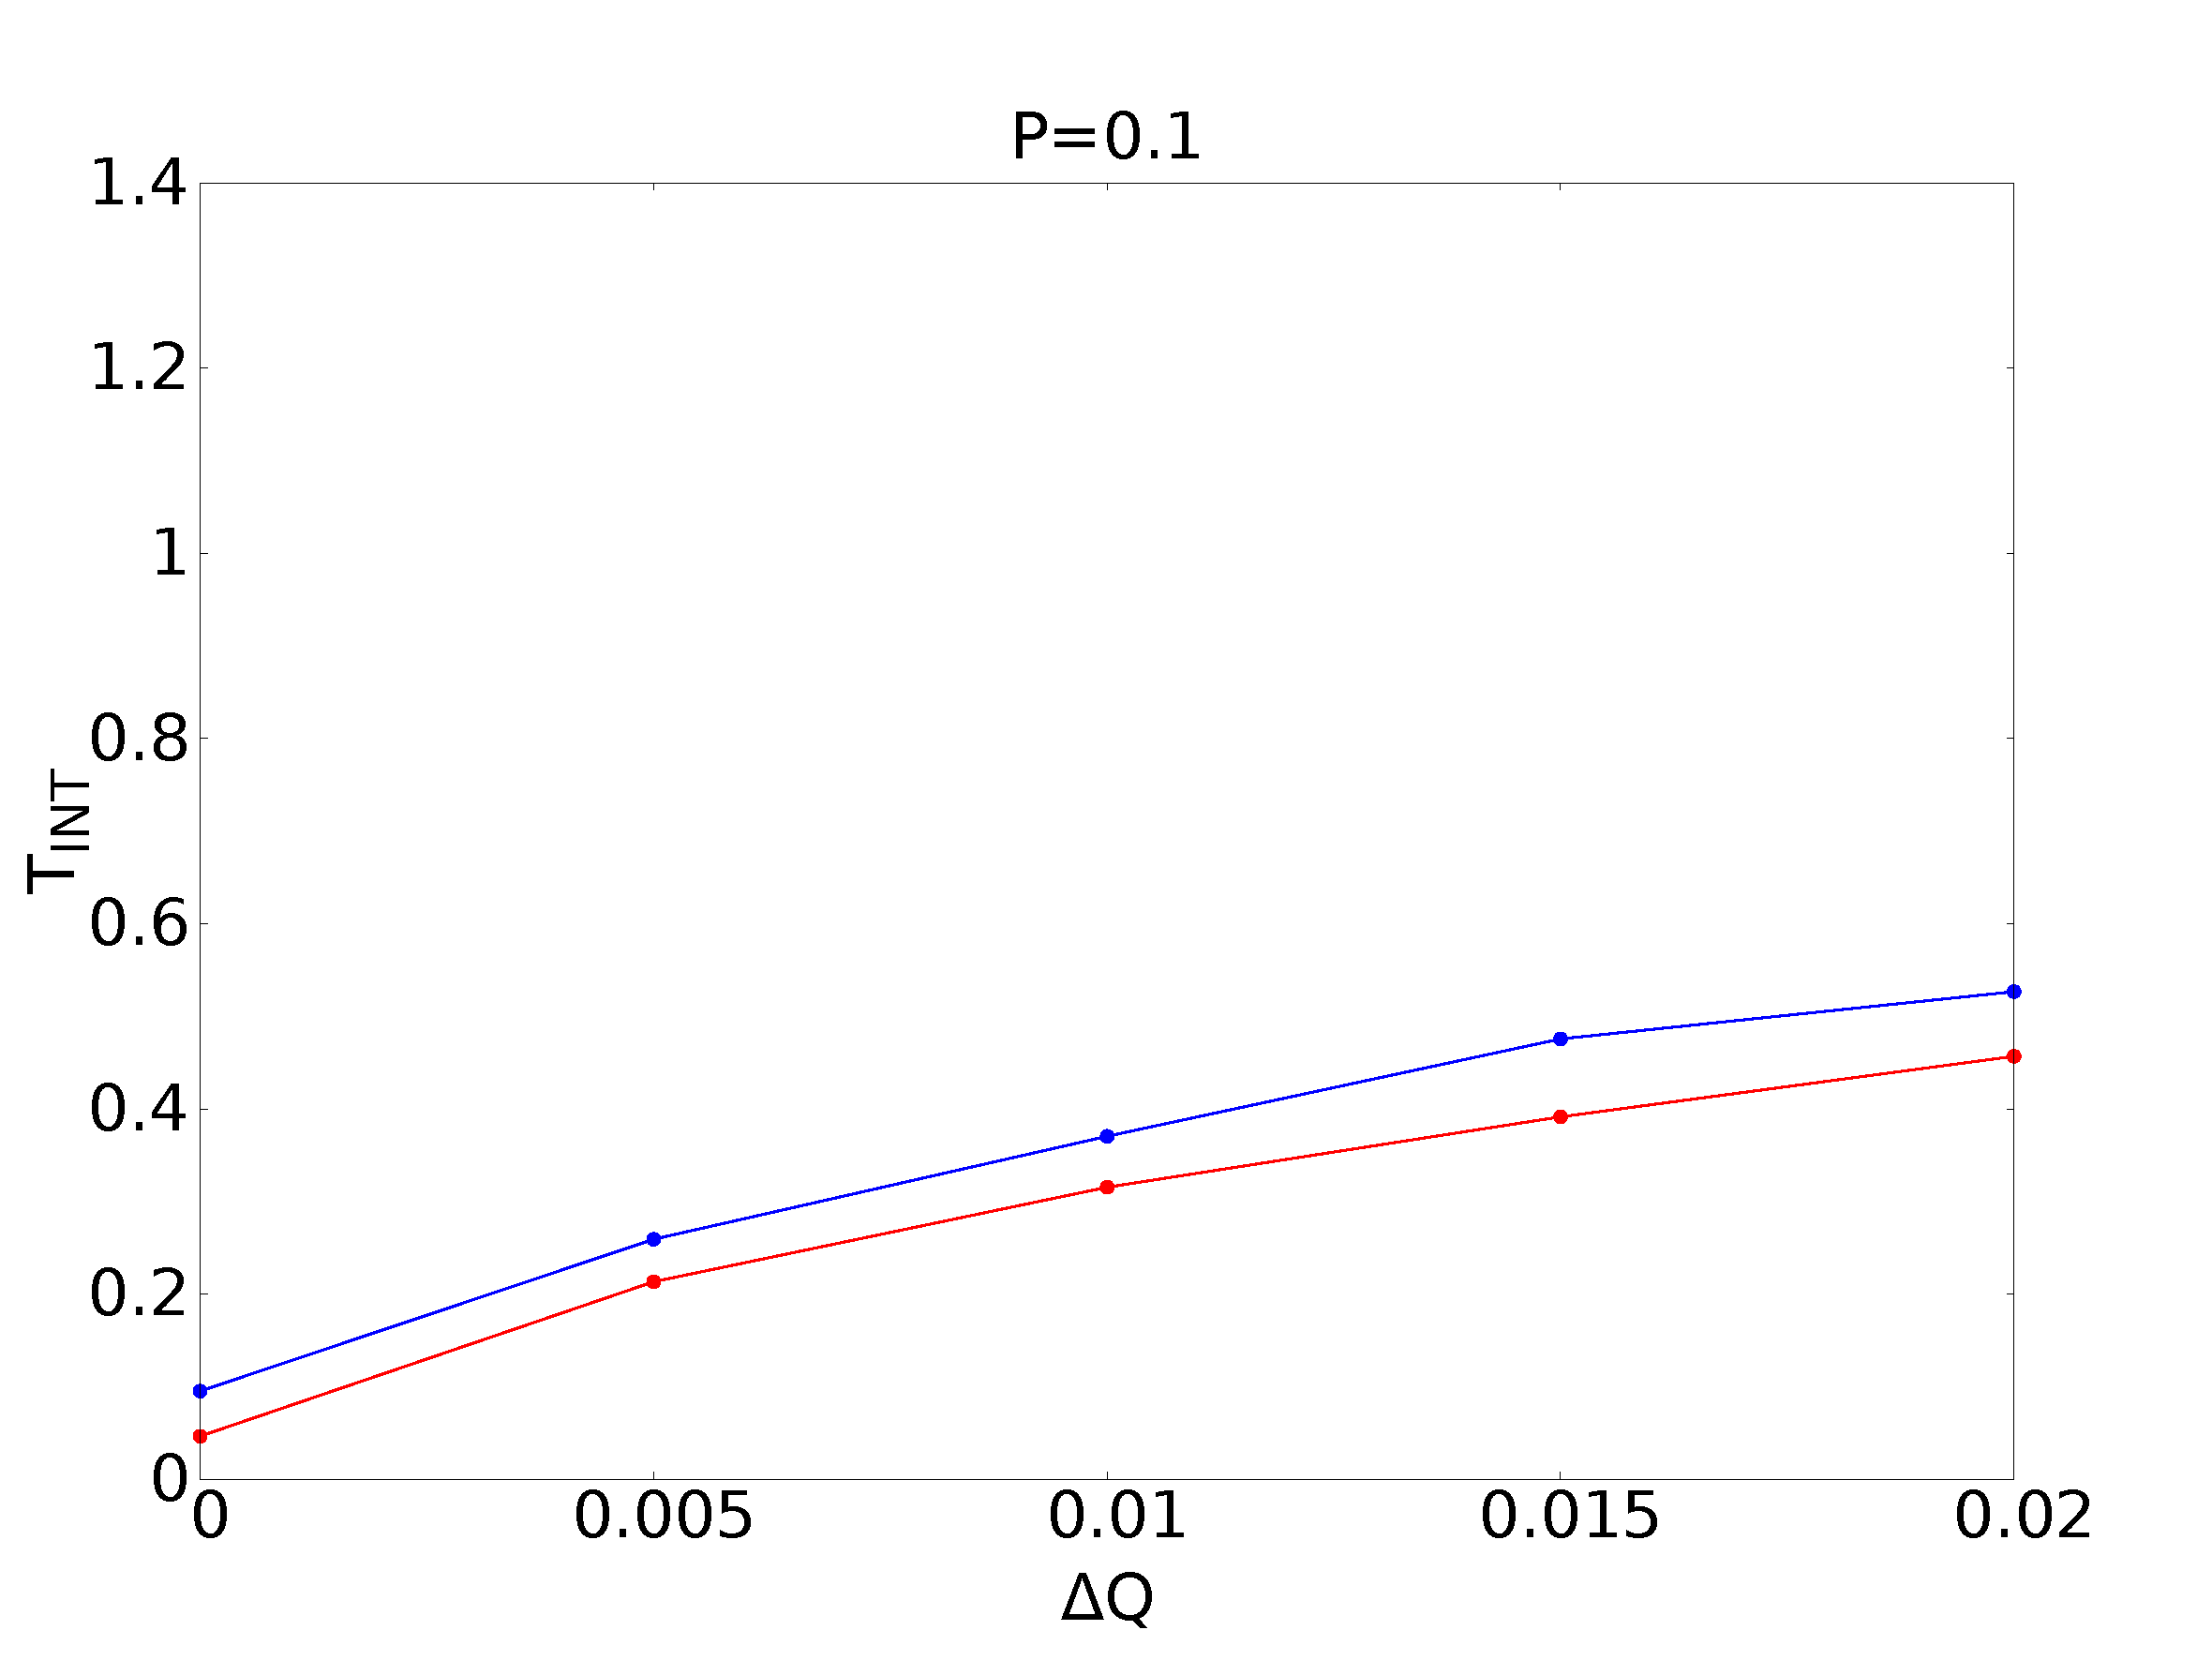
\includegraphics[scale=0.11]{../images/p01_int.pdf}
        \end{subfigure} 
        \
        \begin{subfigure}[t]{0.3\textwidth}
            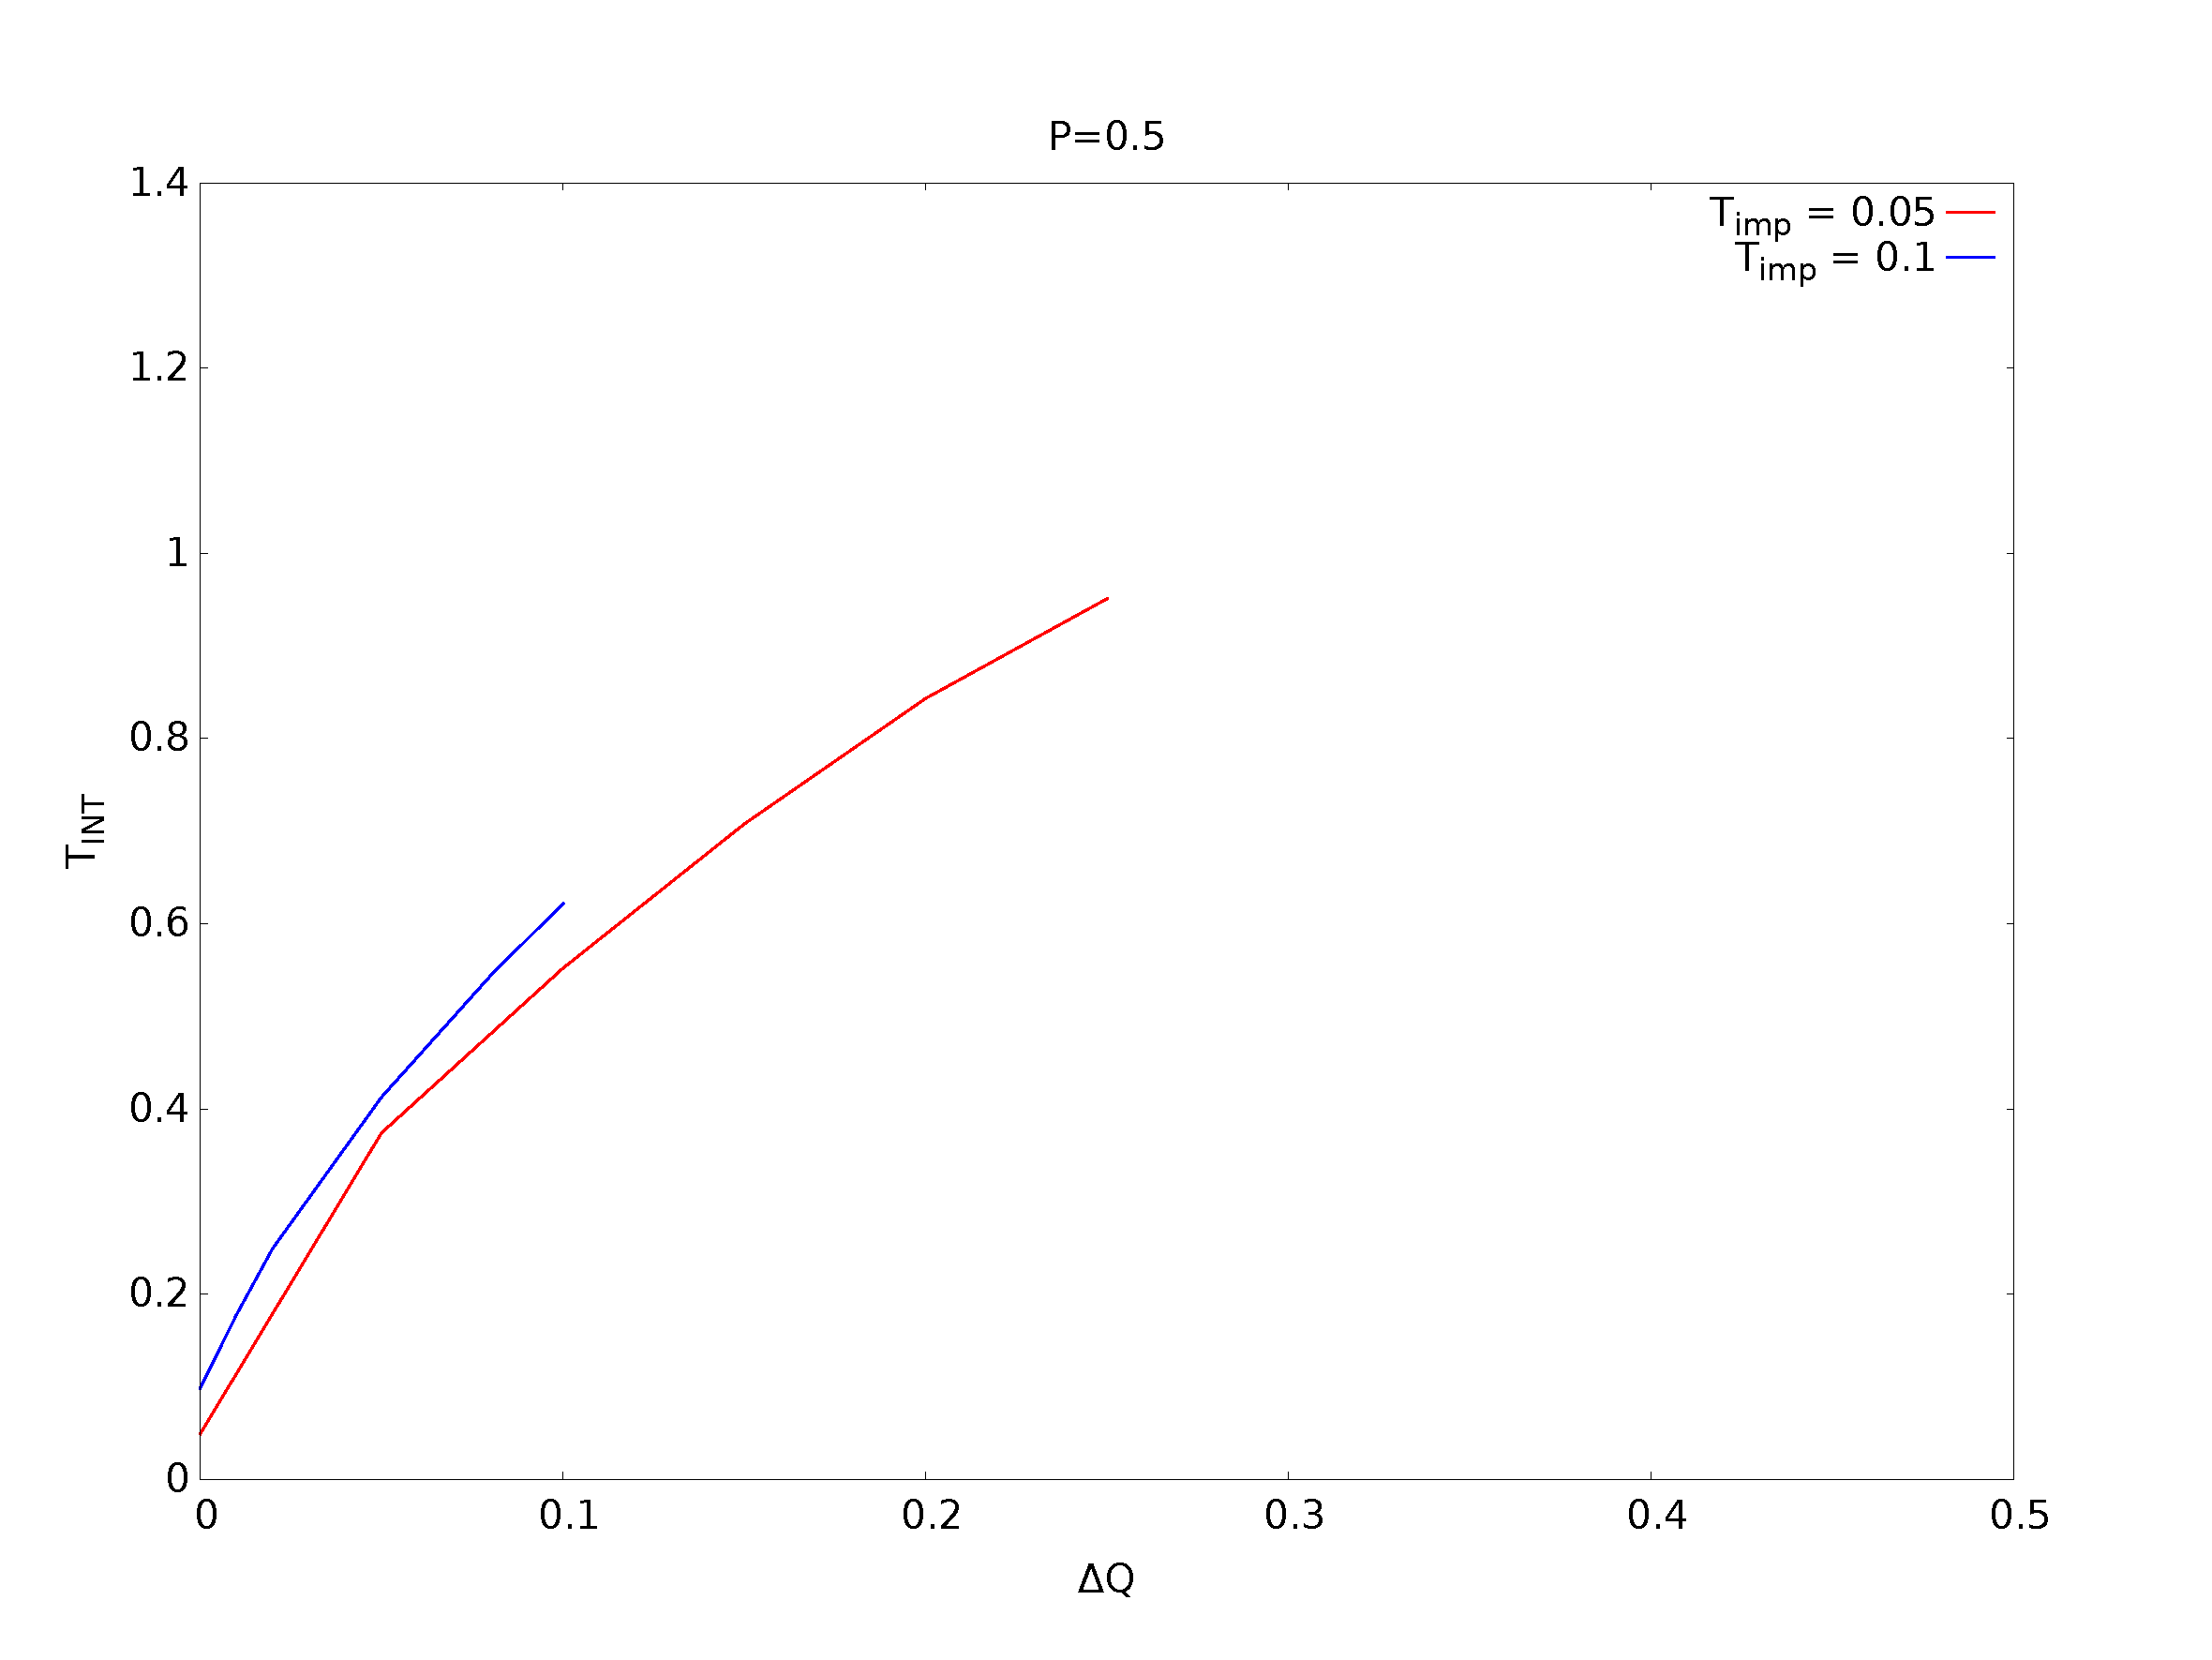
\includegraphics[scale=0.11]{../images/p05_int.pdf}
        \end{subfigure} 
        \
        \begin{subfigure}[t]{0.3\textwidth}
            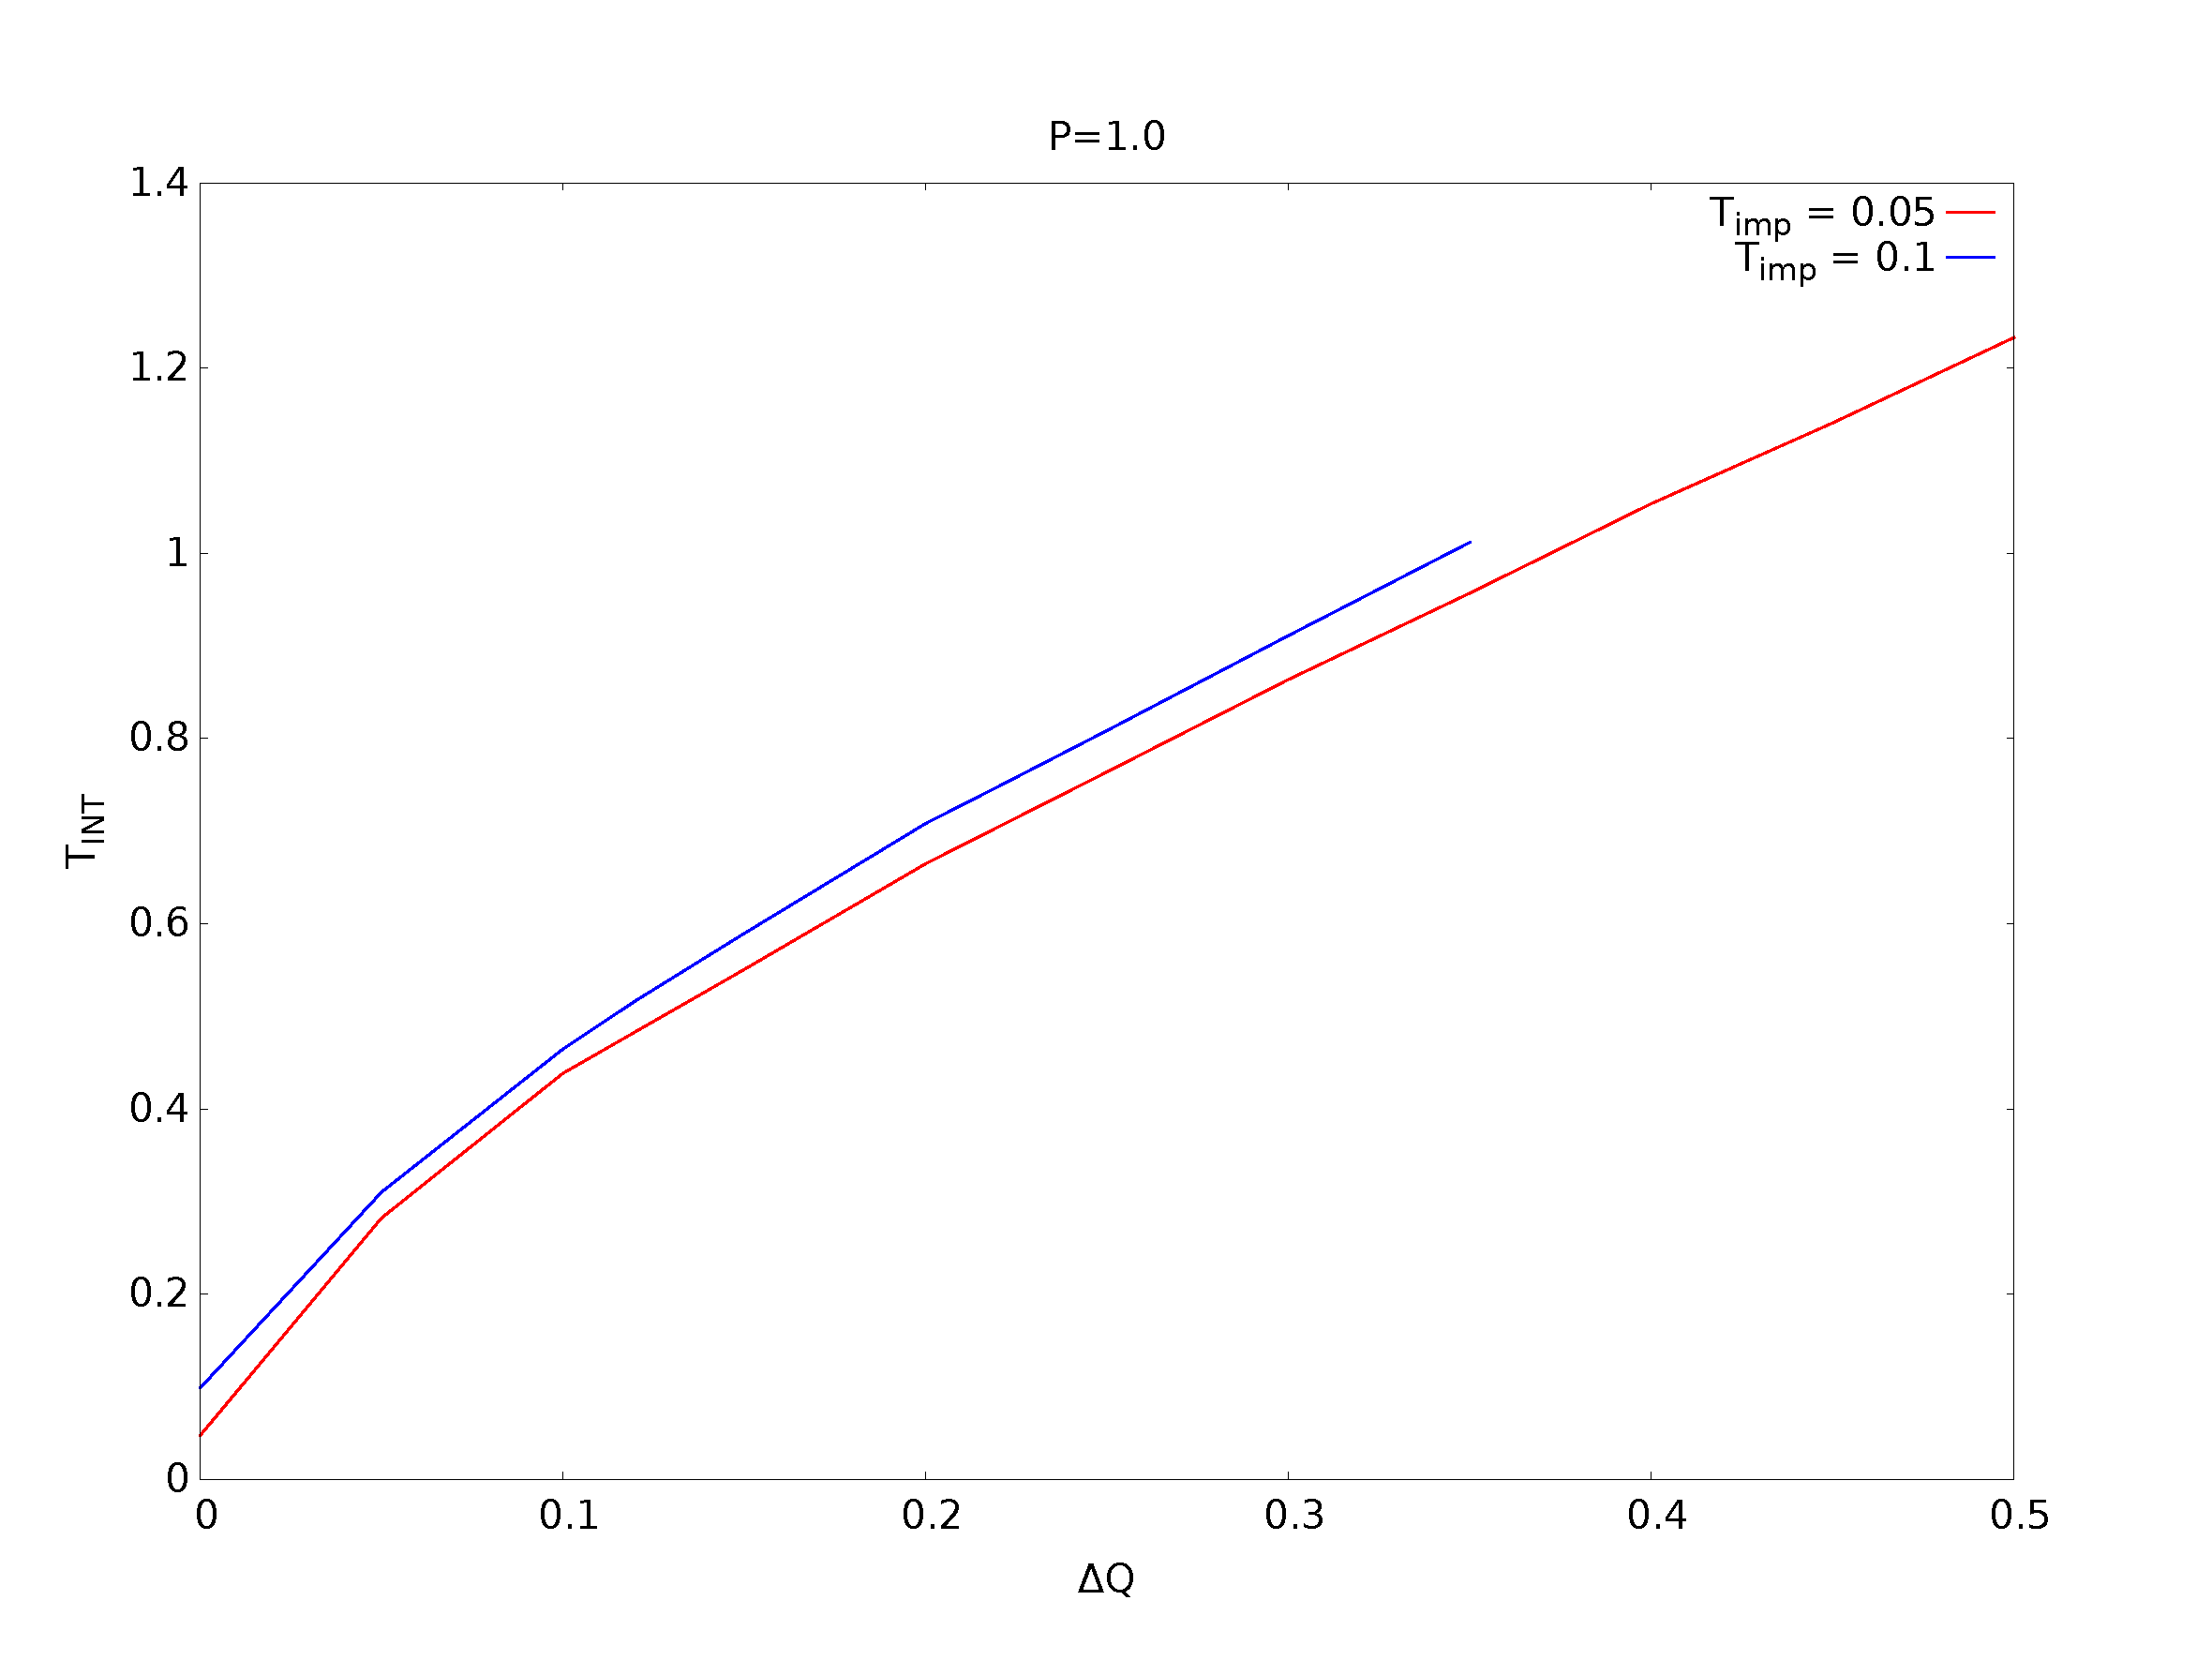
\includegraphics[scale=0.11]{../images/p1_int.pdf}
        \end{subfigure} 
    \end{center}
\end{figure}
\end{frame}

\begin{frame}
\frametitle{Ergebnisse -- Temperatur des ausgehenden Gases}
\begin{figure}
    \begin{center}
        \begin{subfigure}[t]{0.3\textwidth}
            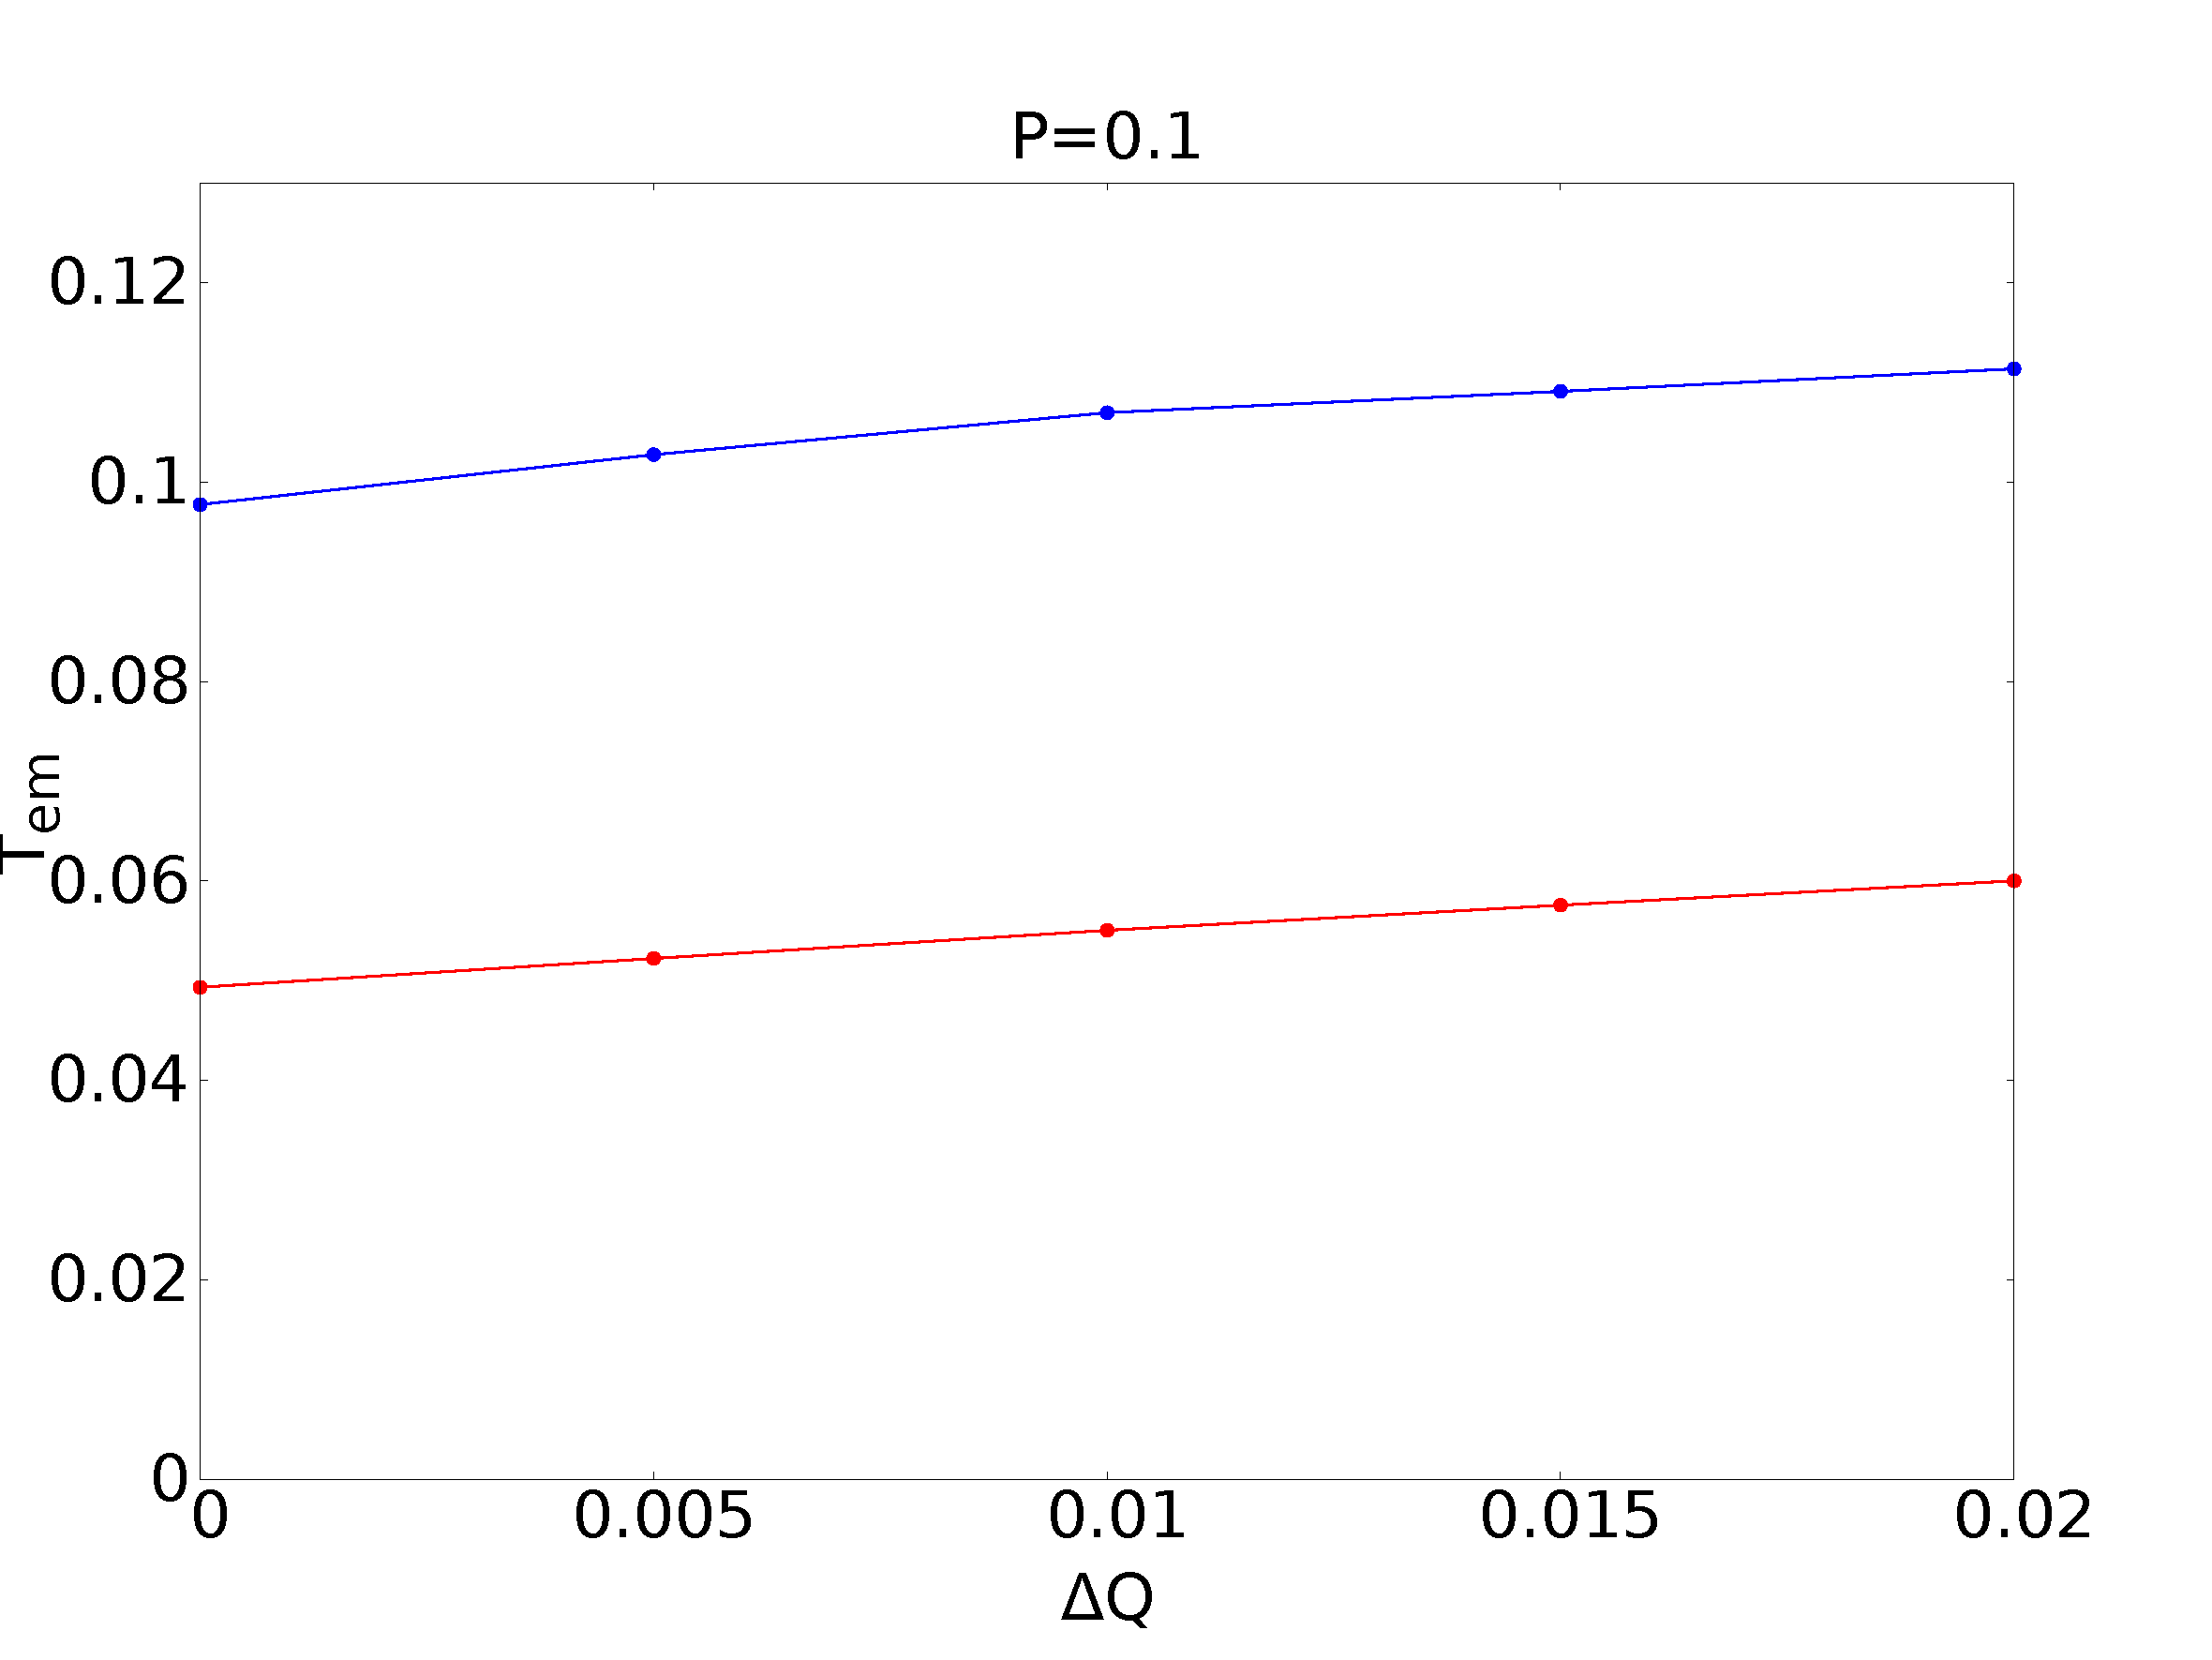
\includegraphics[scale=0.11]{../images/p01_out.pdf}
        \end{subfigure} 
        \
        \begin{subfigure}[t]{0.3\textwidth}
            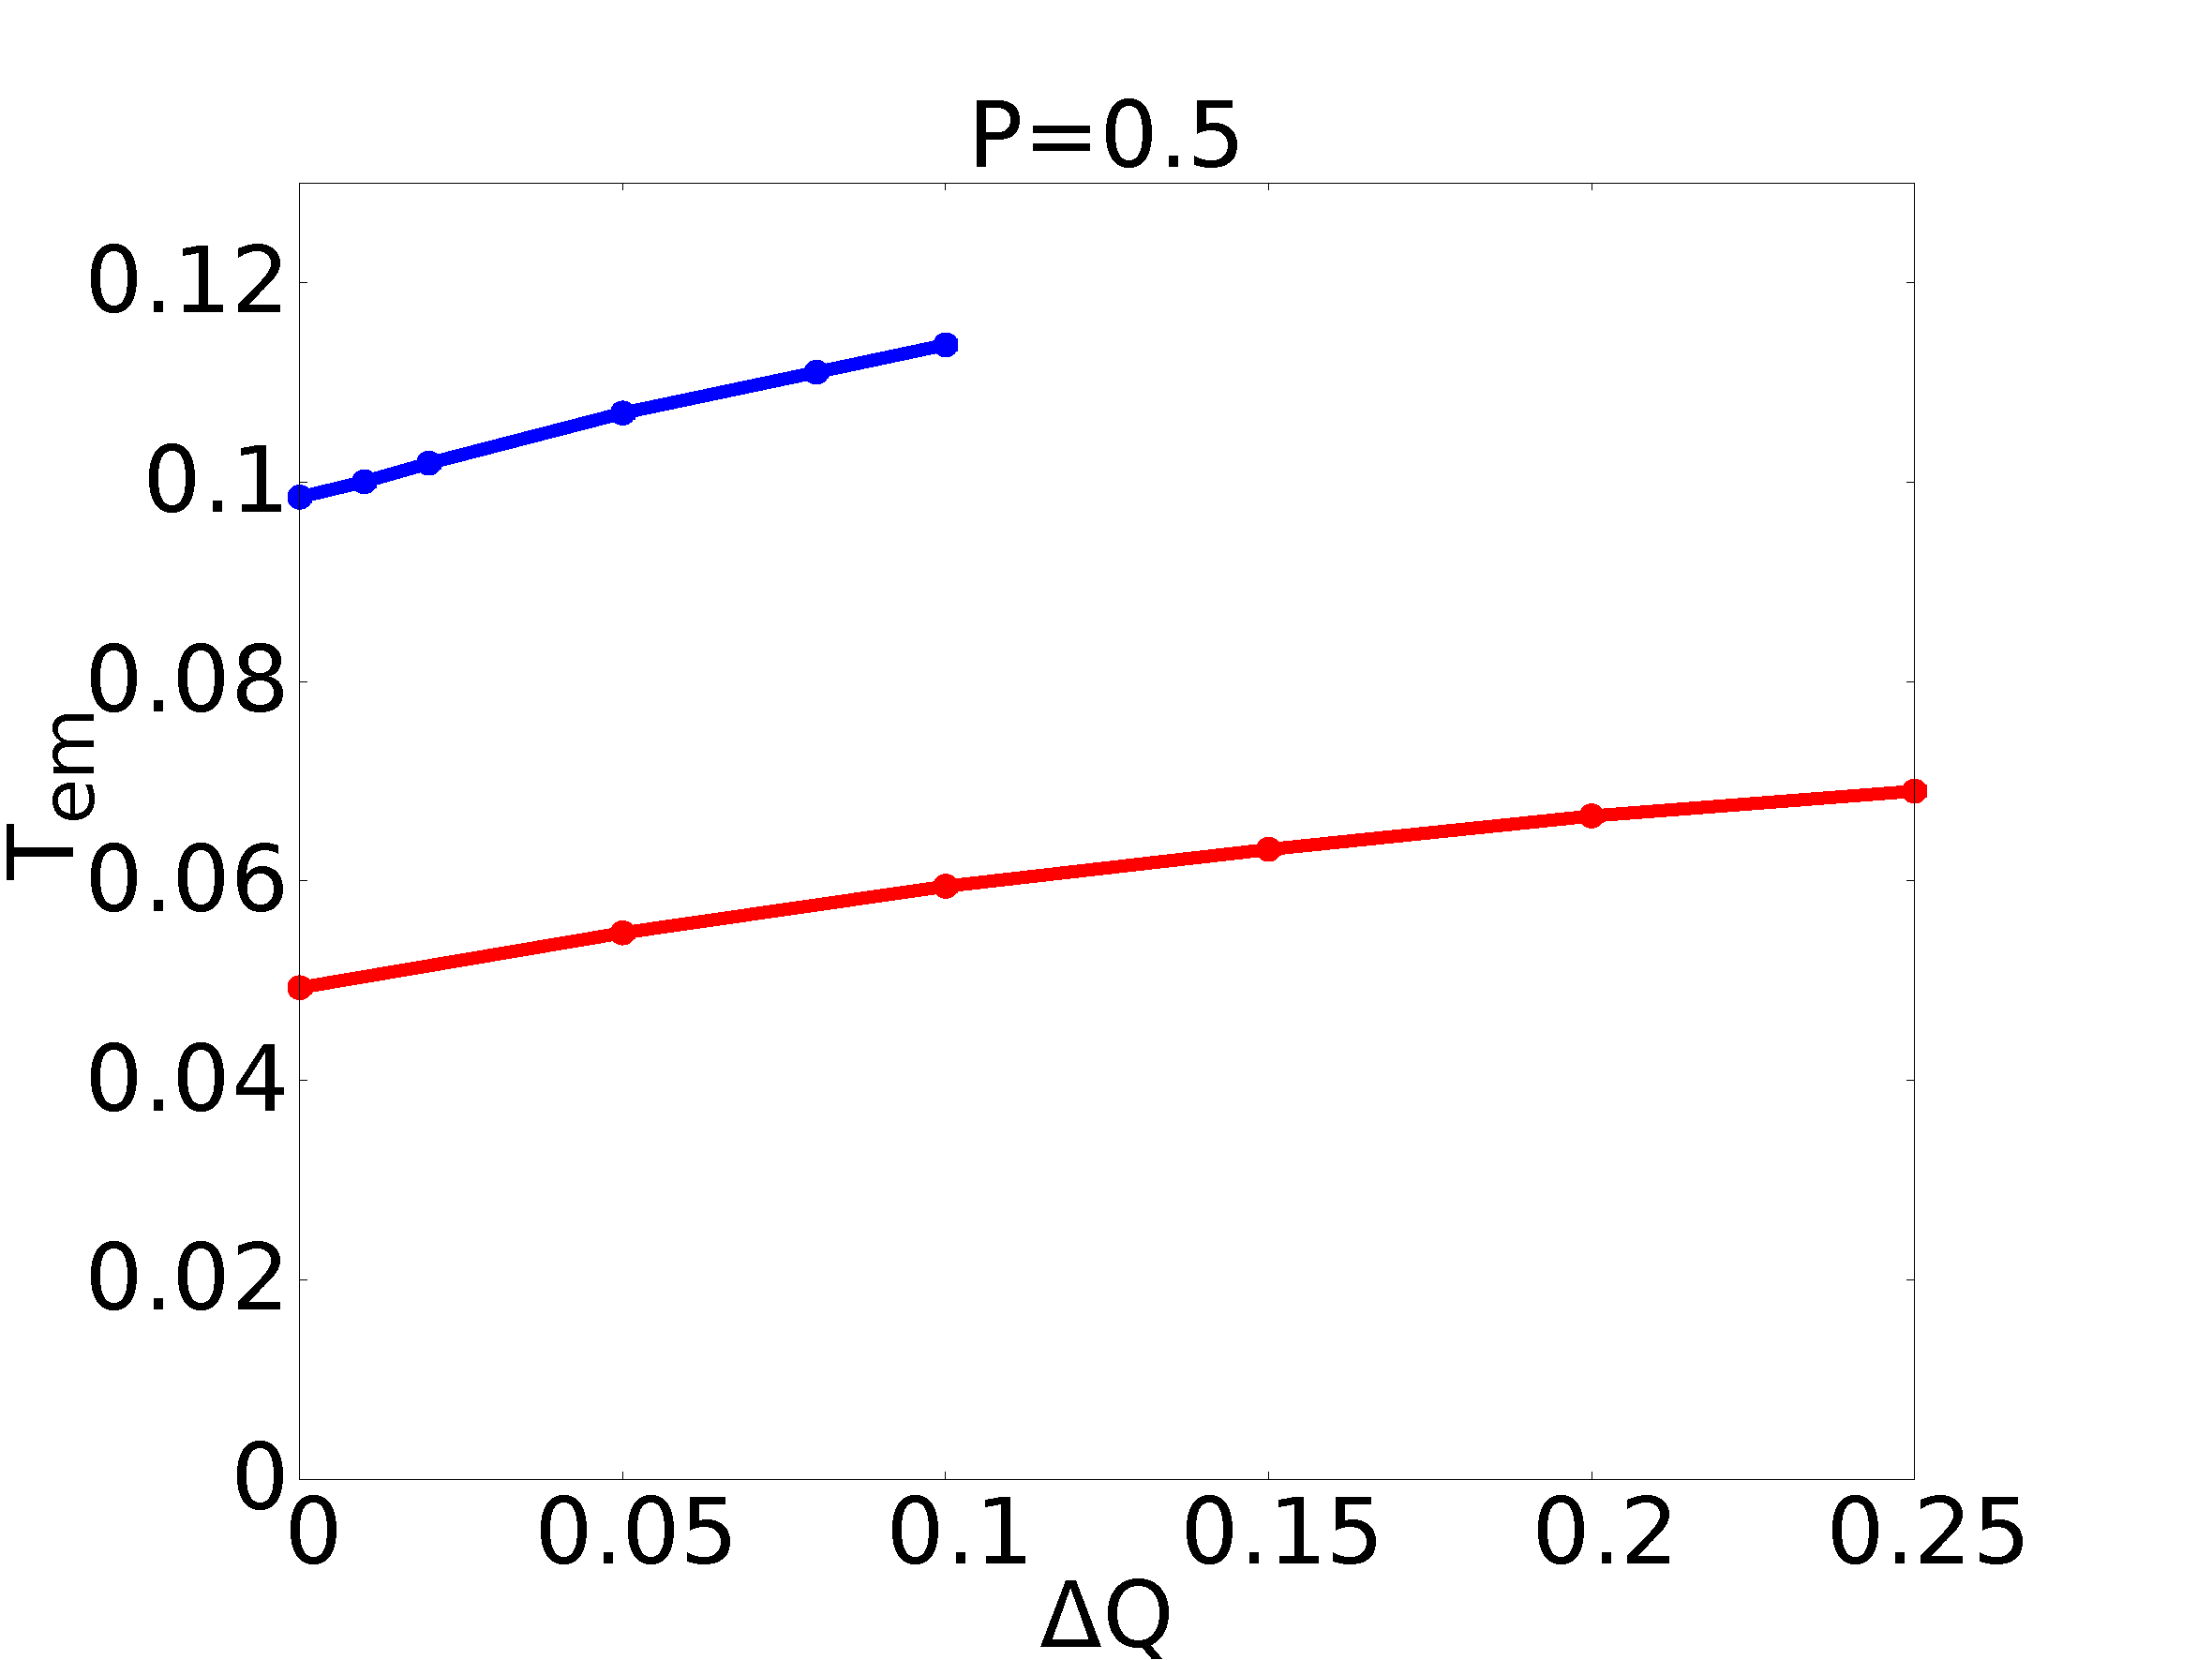
\includegraphics[scale=0.11]{../images/p05_out.pdf}
        \end{subfigure} 
        \
        \begin{subfigure}[t]{0.3\textwidth}
            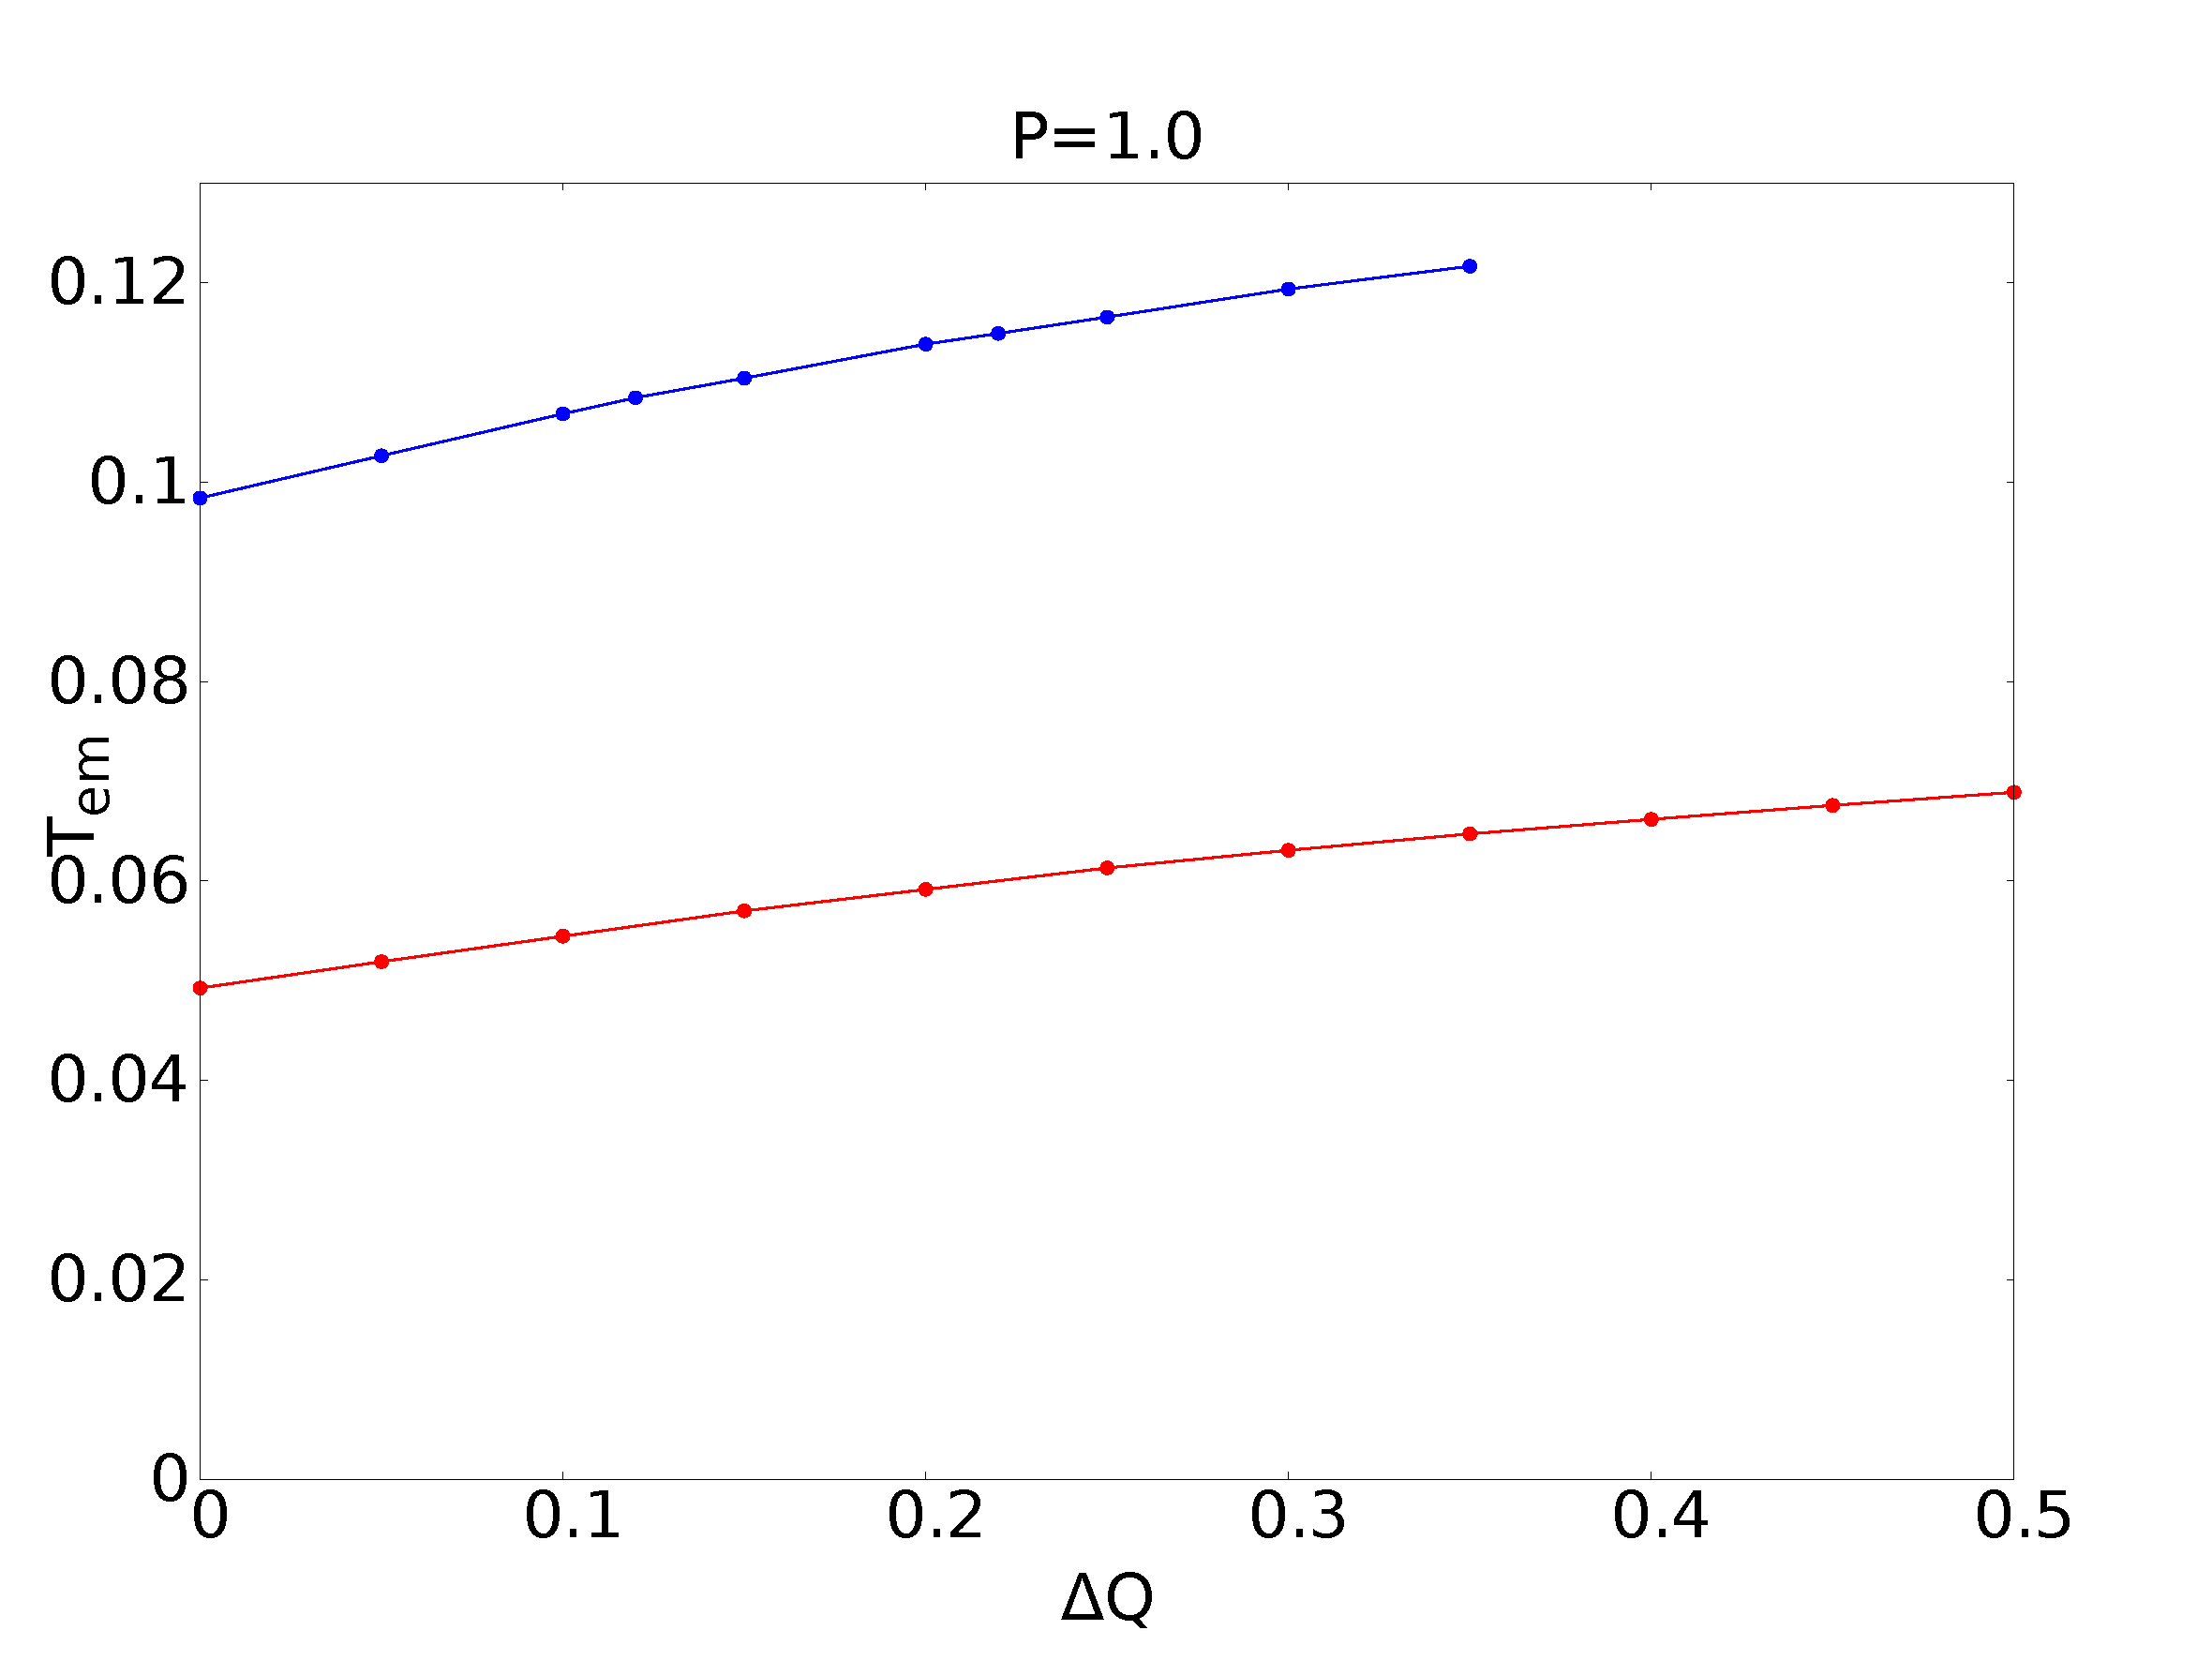
\includegraphics[scale=0.11]{../images/p1_out.pdf}
        \end{subfigure} 
    \end{center}
\end{figure}
\end{frame}

%\begin{frame}
%\frametitle{Vergleich mit Modell}
%Modell für $T_\text{COM}$ von Millen et al.:
%\begin{equation}
    %T_\text{COM} = \frac{T_\text{imp}^{3/2}+\tfrac\pi 8 \ T_\text{em}^{3/2}}{T_\text{imp}^{1/2}+\tfrac\pi8 T_\text{em}^{1/2}}
%\end{equation}
%Vergleich mit Simulation bei $P=0.8$:
%\begin{figure}
    %\begin{center}
        %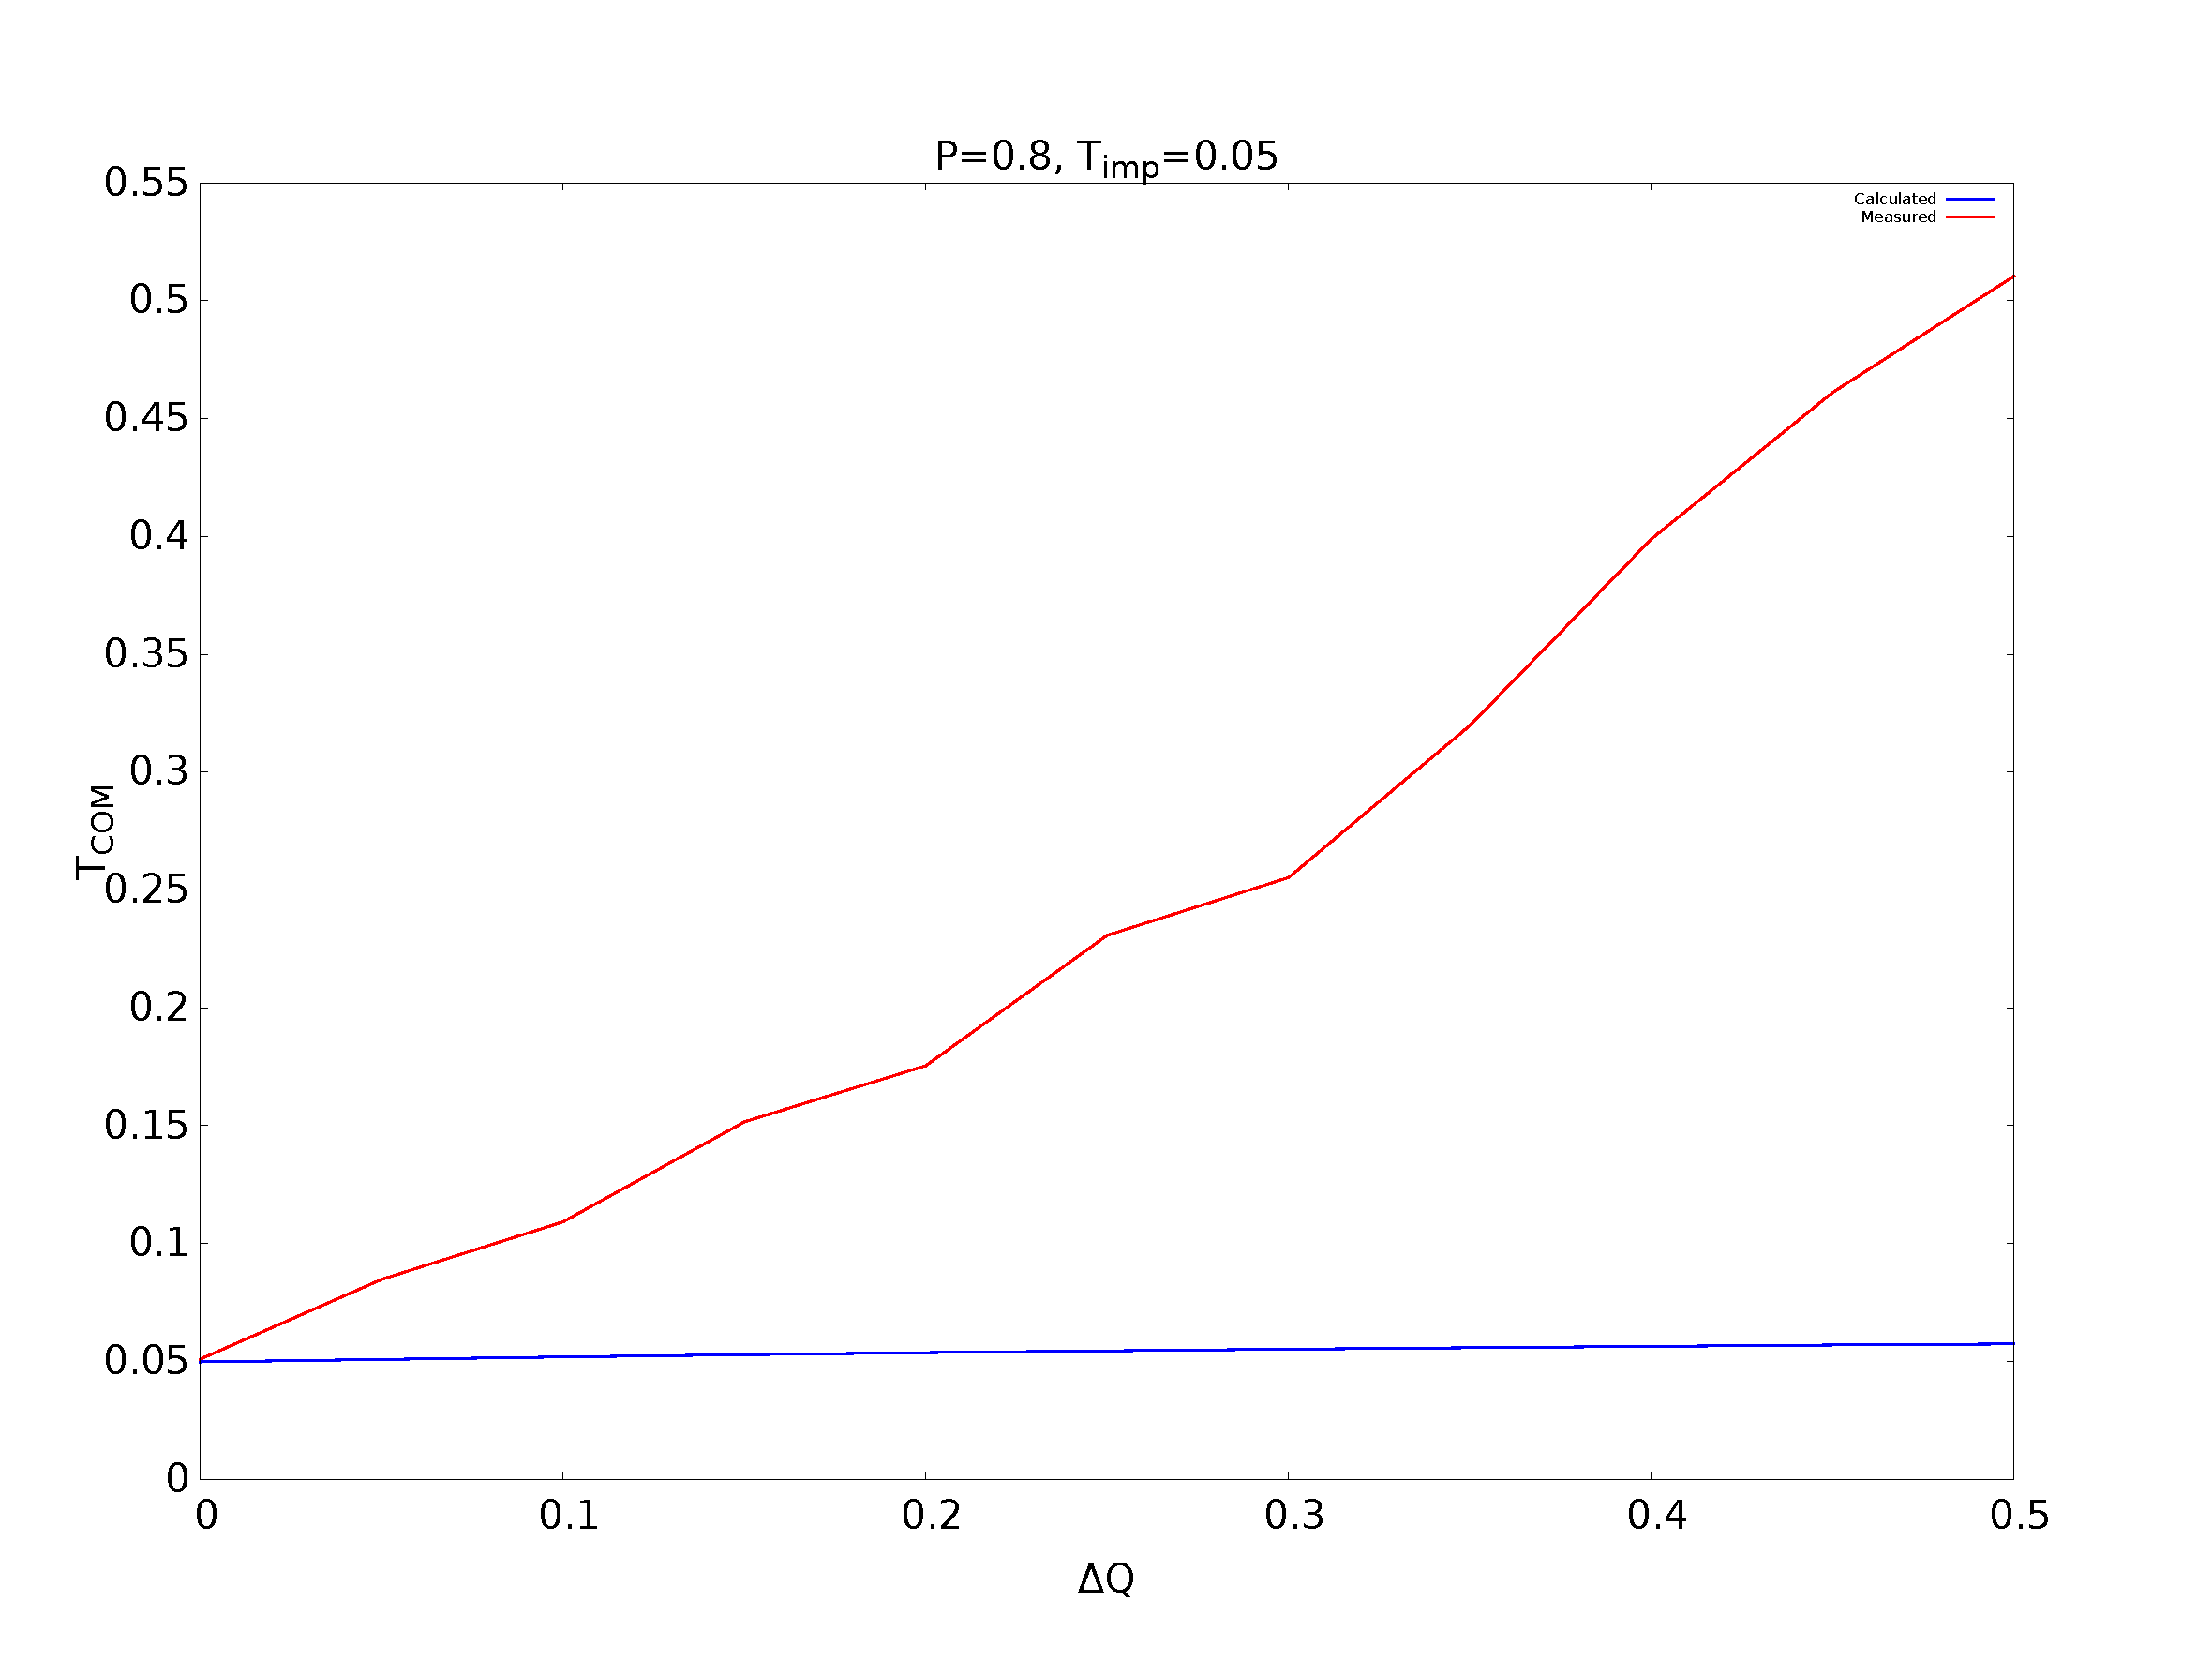
\includegraphics[scale=0.2]{../images/measurevscalc.pdf}
    %\end{center}
%\end{figure}
%\end{frame}


\begin{frame}
\frametitle{Conclusio}
\begin{itemize}
\item Laserleistung beeinflusst die Schwerpunktsbewegung
\item Laserleistung beeinflusst die Temperatur der ausgehenden Gasteilchen 
\item Temperatur der einfallenden Gasteilchen beeinflusst andere Temperaturen 
\end{itemize}
\end{frame}

\bibliography{../references}
\bibliographystyle{unsrt}
\end{document}
